\begin{frame}{%
\protect\hypertarget{objectifs}{%
Objectifs}}

\begin{itemize}
\tightlist
\item
  Comprendre les bases d’un système de gestion de version
\item
  Savoir utiliser git dans un projet

  \begin{itemize}
  \tightlist
  \item
    travailler dans un \emph{repository} local
  \item
    se synchroniser sur un \emph{repository} distant
  \item
    avoir une idée des workflows collaboratifs
  \end{itemize}
\end{itemize}

\end{frame}

\hypertarget{gestion-de-version}{%
\section{Gestion de version}\label{gestion-de-version}}

\begin{frame}{%
\protect\hypertarget{duxe9finition-dun-systuxe8me-de-gestion-de-version}{%
Définition d’un système de gestion de version}}

D’après http://en.wikipedia.org/wiki/Revision\_control

C’est la gestion des changements dans les documents, les programmes, les
grands sites web et de façon plus générale dans les collections
d’information.

Les changements sont généralement identifiés par des codes utilisant des
lettres et des chiffres, appelés le \emph{numéro de révision}. Par
exemple, si un ensemble initial de fichiers sera appelé \emph{révision
1}, après un premier ensemble de changements effectués, il sera appelé
\emph{révision 2} et ainsi de suite.

Chaque révision est associée à un horodatage (timestamp) et à un auteur.

Les révisions pourront être comparées, restaurées et dans certains cas
fusionnées.

\end{frame}

\begin{frame}{%
\protect\hypertarget{cas-dusage-1-conservation-de-lhistorique}{%
Cas d’usage 1: conservation de l’historique}}

La vie de votre programme/document est enregistrée depuis son début

\begin{itemize}
\tightlist
\item
  A tout moment on peut revenir à la version précédente\footnote<.->{si
    vous n’êtes pas contents de vos modifs}
\item
  L’historique est accessible, on peut inspecter chaque
  révision\footnote<.->{pour comprendre et résoudre les bugs}

  \begin{itemize}
  \tightlist
  \item
    quand a-t-elle été faite ?
  \item
    qui l’a faite ?
  \item
    quelle était la nature du changement ?
  \item
    pourquoi ?
  \item
    dans quel contexte ?
  \end{itemize}
\item
  tous les changements effacés restent accessible dans l’historique
\end{itemize}

\end{frame}

\begin{frame}{%
\protect\hypertarget{cas-dusage-2-travailler-uxe0-plusieurs}{%
Cas d’usage 2 : travailler à plusieurs}}

Les outils de gestion de version vous aident à :

\begin{itemize}
\tightlist
\item
  partager une collection de fichiers avec votre équipe
\item
  fusionner les changements effectués par les autres
\item
  vous assurer que rien n’est effacé par erreur
\item
  \sout{savoir qui engu\ldots{} quand quelque chose ne marche pas}
\end{itemize}

\end{frame}

\begin{frame}{%
\protect\hypertarget{cas-dusage-3-les-branches}{%
Cas d’usage 3 : les branches}}

Il arrive qu’on ait de multiples versions d’un programme, matérialisées
comme des branches. Par exemple :

\begin{itemize}
\tightlist
\item
  une branche principale
\item
  une branche de maintenance (pour corriger les bugs dans les anciennes
  versions)
\item
  une branche de développement (pour effectuer des changements de fond)
\item
  une branche de \emph{release} (pour figer le code avant une livraison)
\end{itemize}

Les outils de gestion de version vont vous aider à :

\begin{itemize}
\tightlist
\item
  gérer plusieurs branches de façon concurrente
\item
  fusionner (tout ou partie) des branches
\end{itemize}

\end{frame}

\begin{frame}{%
\protect\hypertarget{cas-dusage-4-travailler-avec-des-contributeurs-externes}{%
Cas d’usage 4 : travailler avec des contributeurs externes}}

Les outils de gestion de version vous aident à travailler avec des
développeurs externes :

\begin{itemize}
\tightlist
\item
  cela leur donne de la visibilité sur ce qui se passe dans le projet
\item
  cela les aide à soumettre des modifications (\emph{patches}) et vous
  aide à intégrer leurs patches
\item
  permet aux développeurs de créer leur propre version du projet, puis à
  revenir vers la branche principale
\end{itemize}

\end{frame}

\begin{frame}[fragile]{%
\protect\hypertarget{cas-dusage-5-passage-uxe0-luxe9chelle}{%
Cas d’usage 5 : passage à l’échelle}}

\begin{itemize}
\tightlist
\item
  Quelques éléments sur le noyau de Linux

  \begin{itemize}
  \tightlist
  \item
    Linus Torvald a créé \texttt{git} pour gérer le flot de révisions !
  \item
    environ 10000 changements dans chaque nouvelle version (tous les 2-3
    mois)
  \item
    plus de 1000 contributeurs
  \end{itemize}
\end{itemize}

\end{frame}

\begin{frame}{%
\protect\hypertarget{illustrations-le-repository}{%
Illustrations : le repository}}

\begin{columns}[T]
\begin{column}{0.40\textwidth}
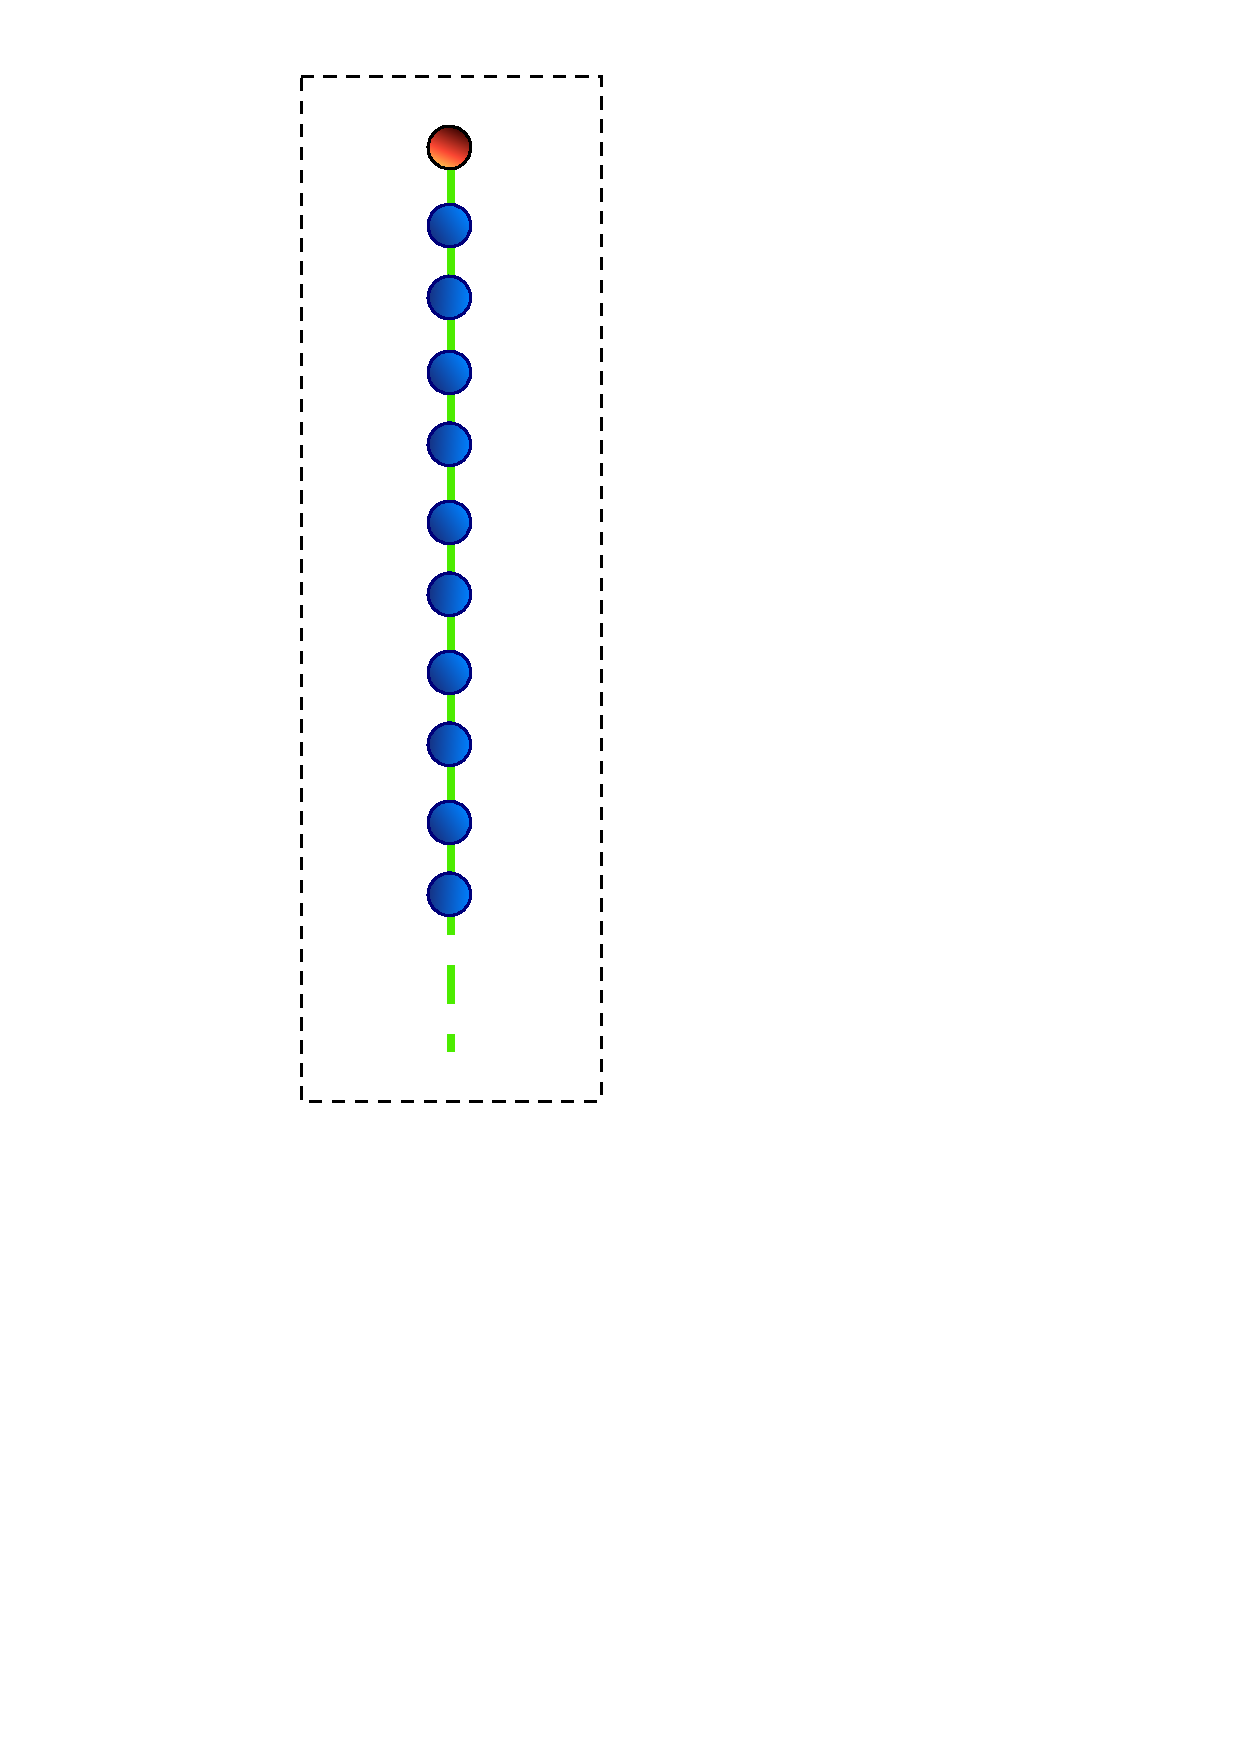
\includegraphics[height=1.5\textwidth]{images/repo.pdf}
\end{column}

\begin{column}{0.60\textwidth}
Il contient l’historique complet du projet (toutes les révisions depuis
le début)
\end{column}
\end{columns}

\end{frame}

\begin{frame}{%
\protect\hypertarget{illustrations-les-ruxe9visions}{%
Illustrations : les révisions}}

\begin{columns}[T]
\begin{column}{0.40\textwidth}
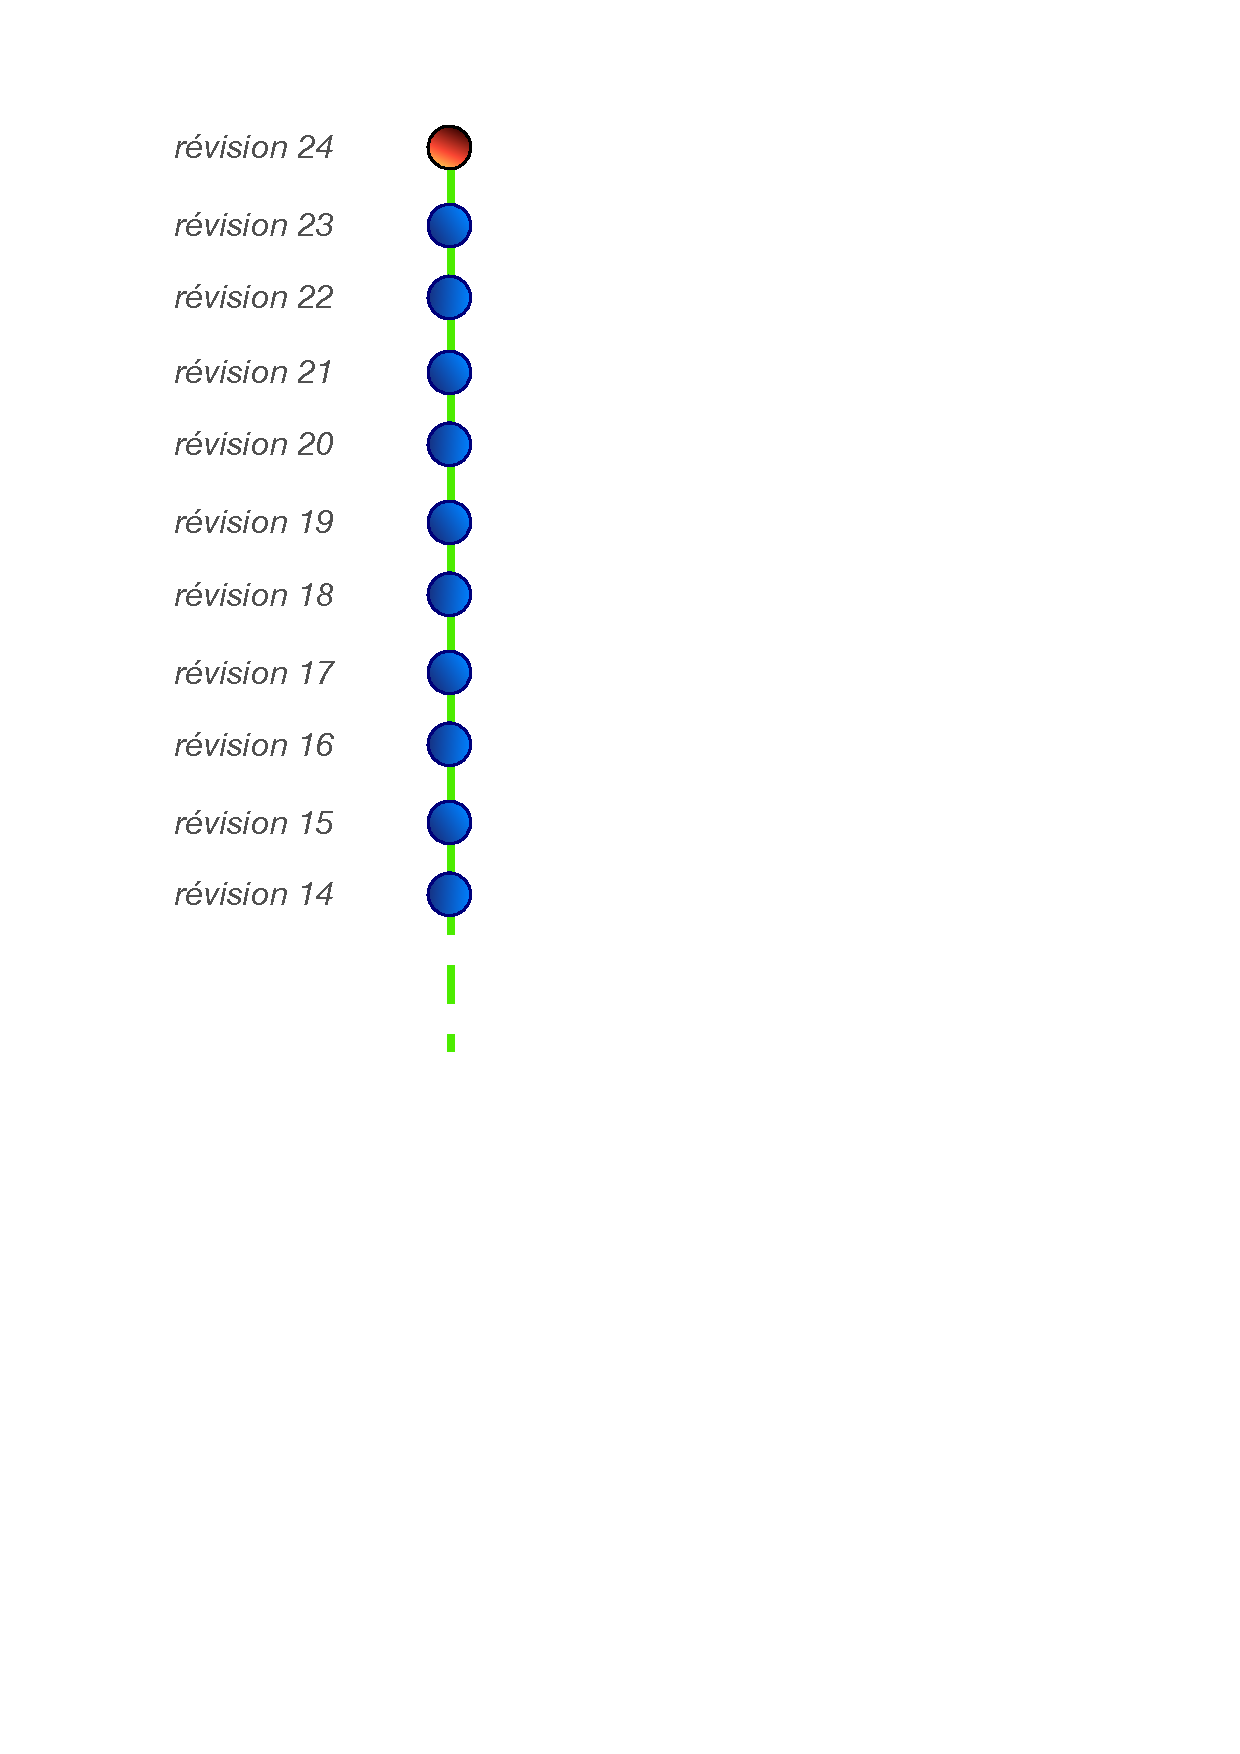
\includegraphics[height=1.5\textwidth]{images/revisions.pdf}
\end{column}

\begin{column}{0.60\textwidth}
Chaque révision

\begin{itemize}
\tightlist
\item
  introduit des changements par rapport à la révision précédente
\item
  a un auteur identifié
\item
  est horodatée
\item
  contient un message qui décrit les changements
\end{itemize}
\end{column}
\end{columns}

\end{frame}

\begin{frame}{%
\protect\hypertarget{illustrations-head}{%
Illustrations : HEAD}}

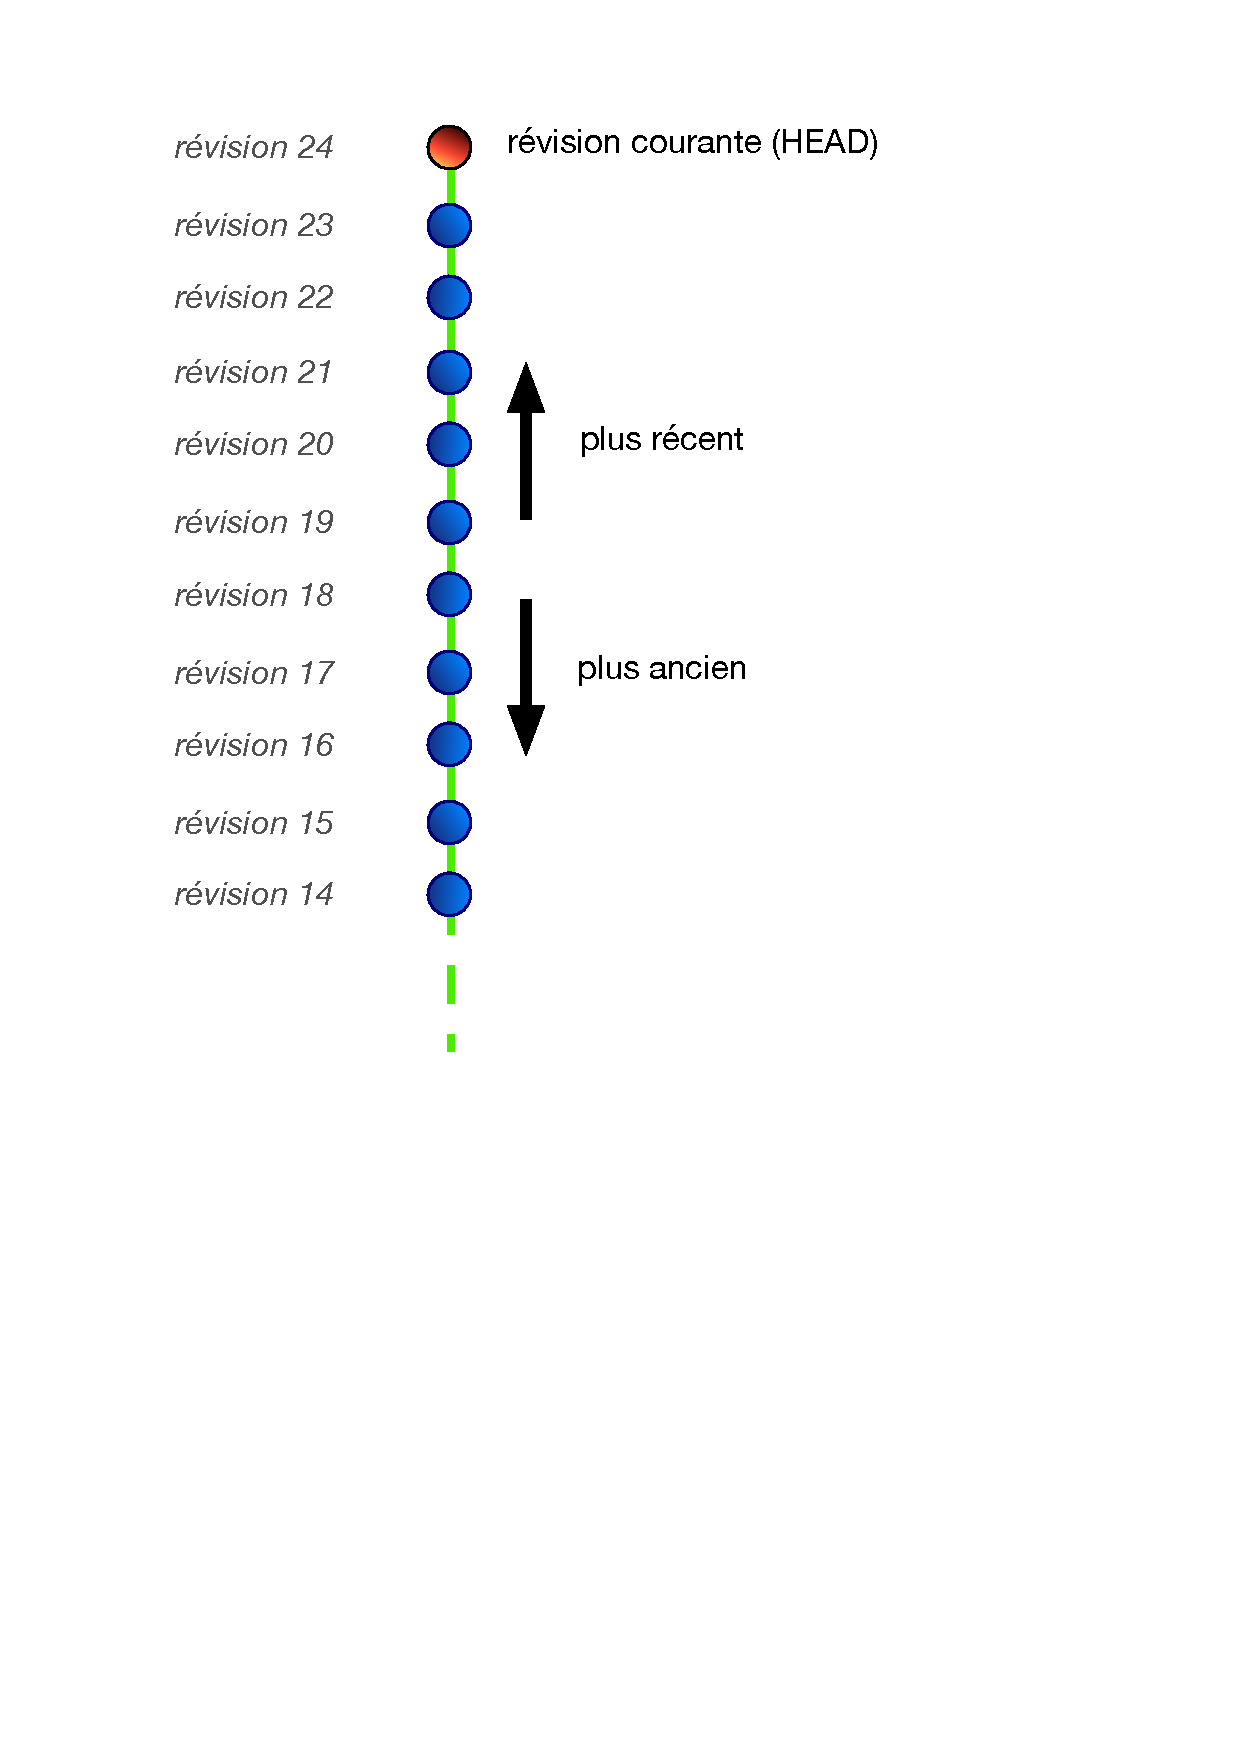
\includegraphics[height=1\textwidth]{images/head.pdf}

\end{frame}

\begin{frame}{%
\protect\hypertarget{illustrations-les-tags-uxe9tiquettes}{%
Illustrations : les tags (étiquettes)}}

\begin{columns}[T]
\begin{column}{0.40\textwidth}
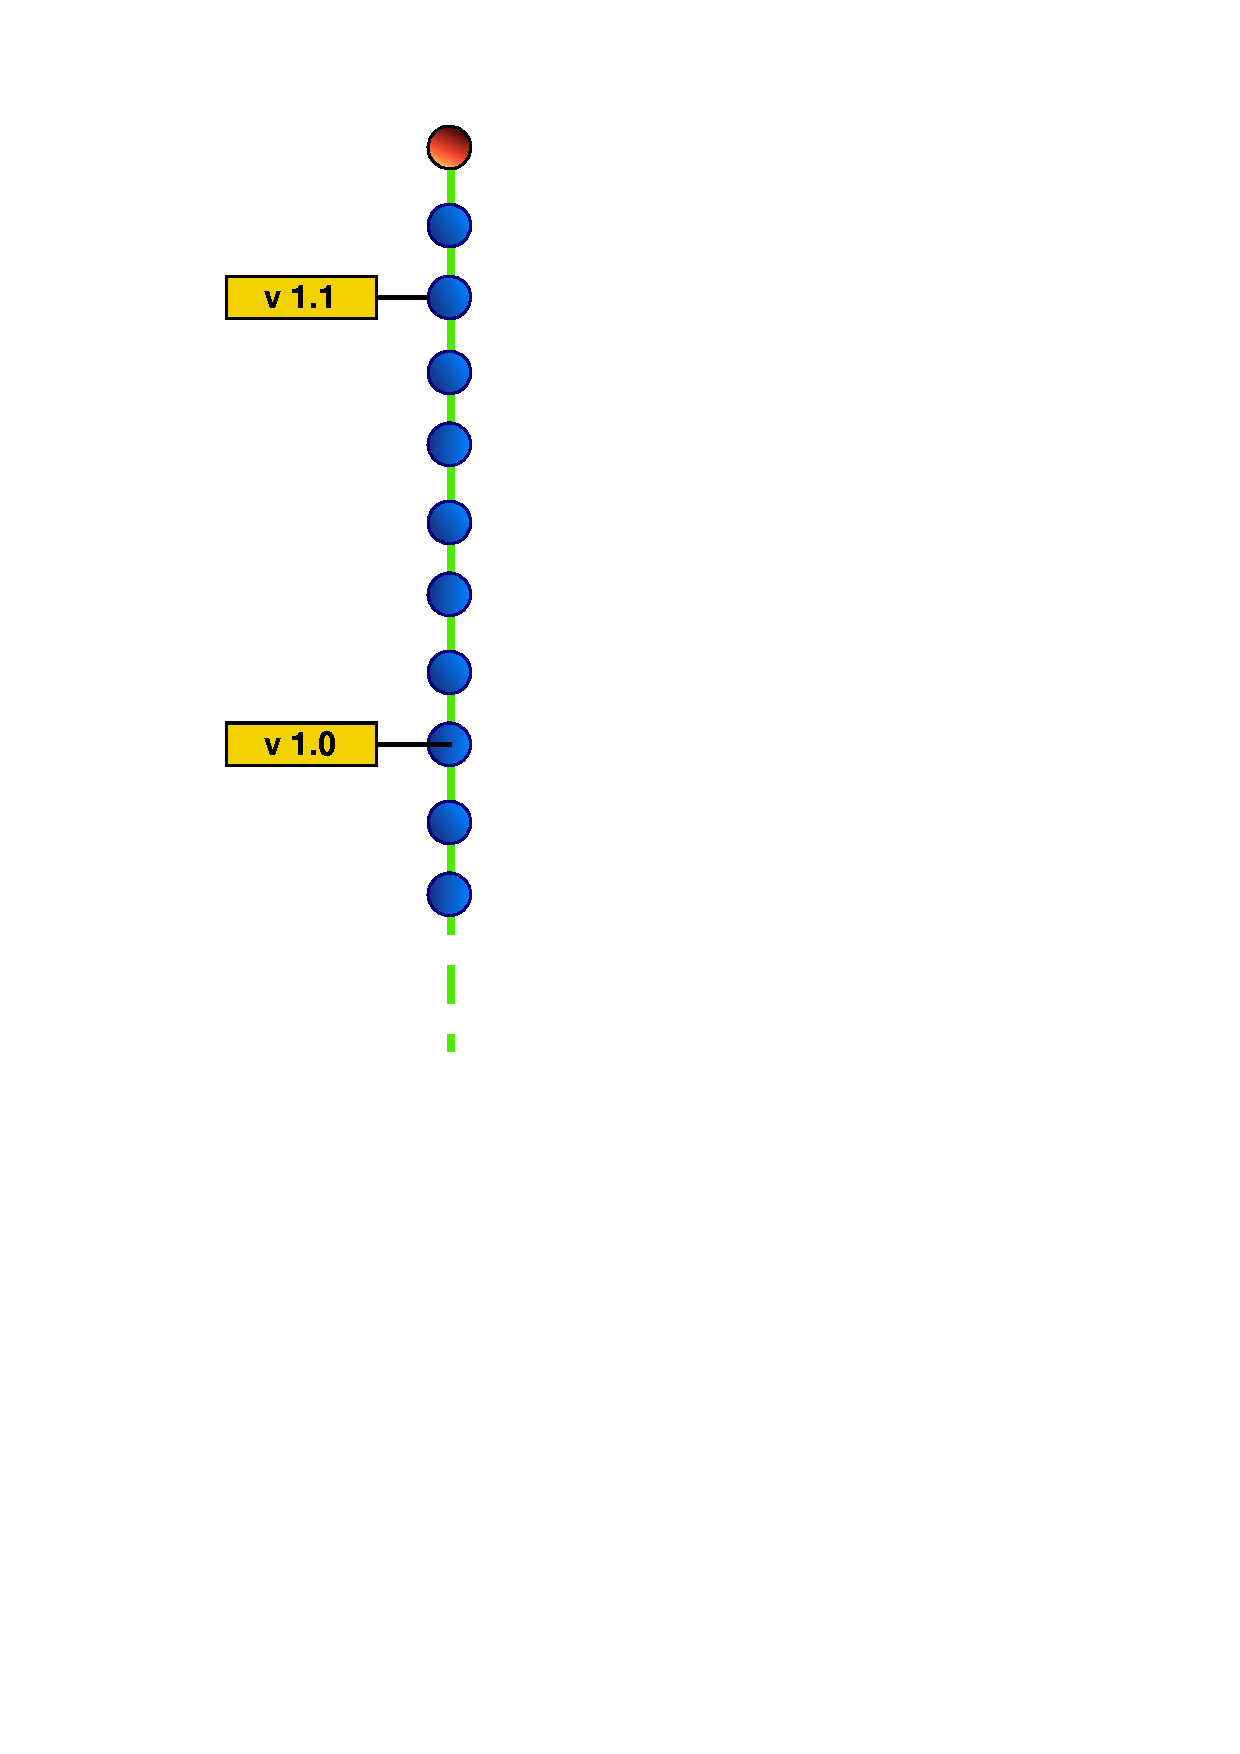
\includegraphics[height=1.5\textwidth]{images/tags.pdf}
\end{column}

\begin{column}{0.60\textwidth}
Un tag

\begin{itemize}
\tightlist
\item
  identifie une révision particulière
\item
  par exemple les livraisons du logiciel
\end{itemize}
\end{column}
\end{columns}

\end{frame}

\begin{frame}[fragile]{%
\protect\hypertarget{illustrations-les-branches}{%
Illustrations : les branches}}

\begin{columns}[T]
\begin{column}{0.40\textwidth}
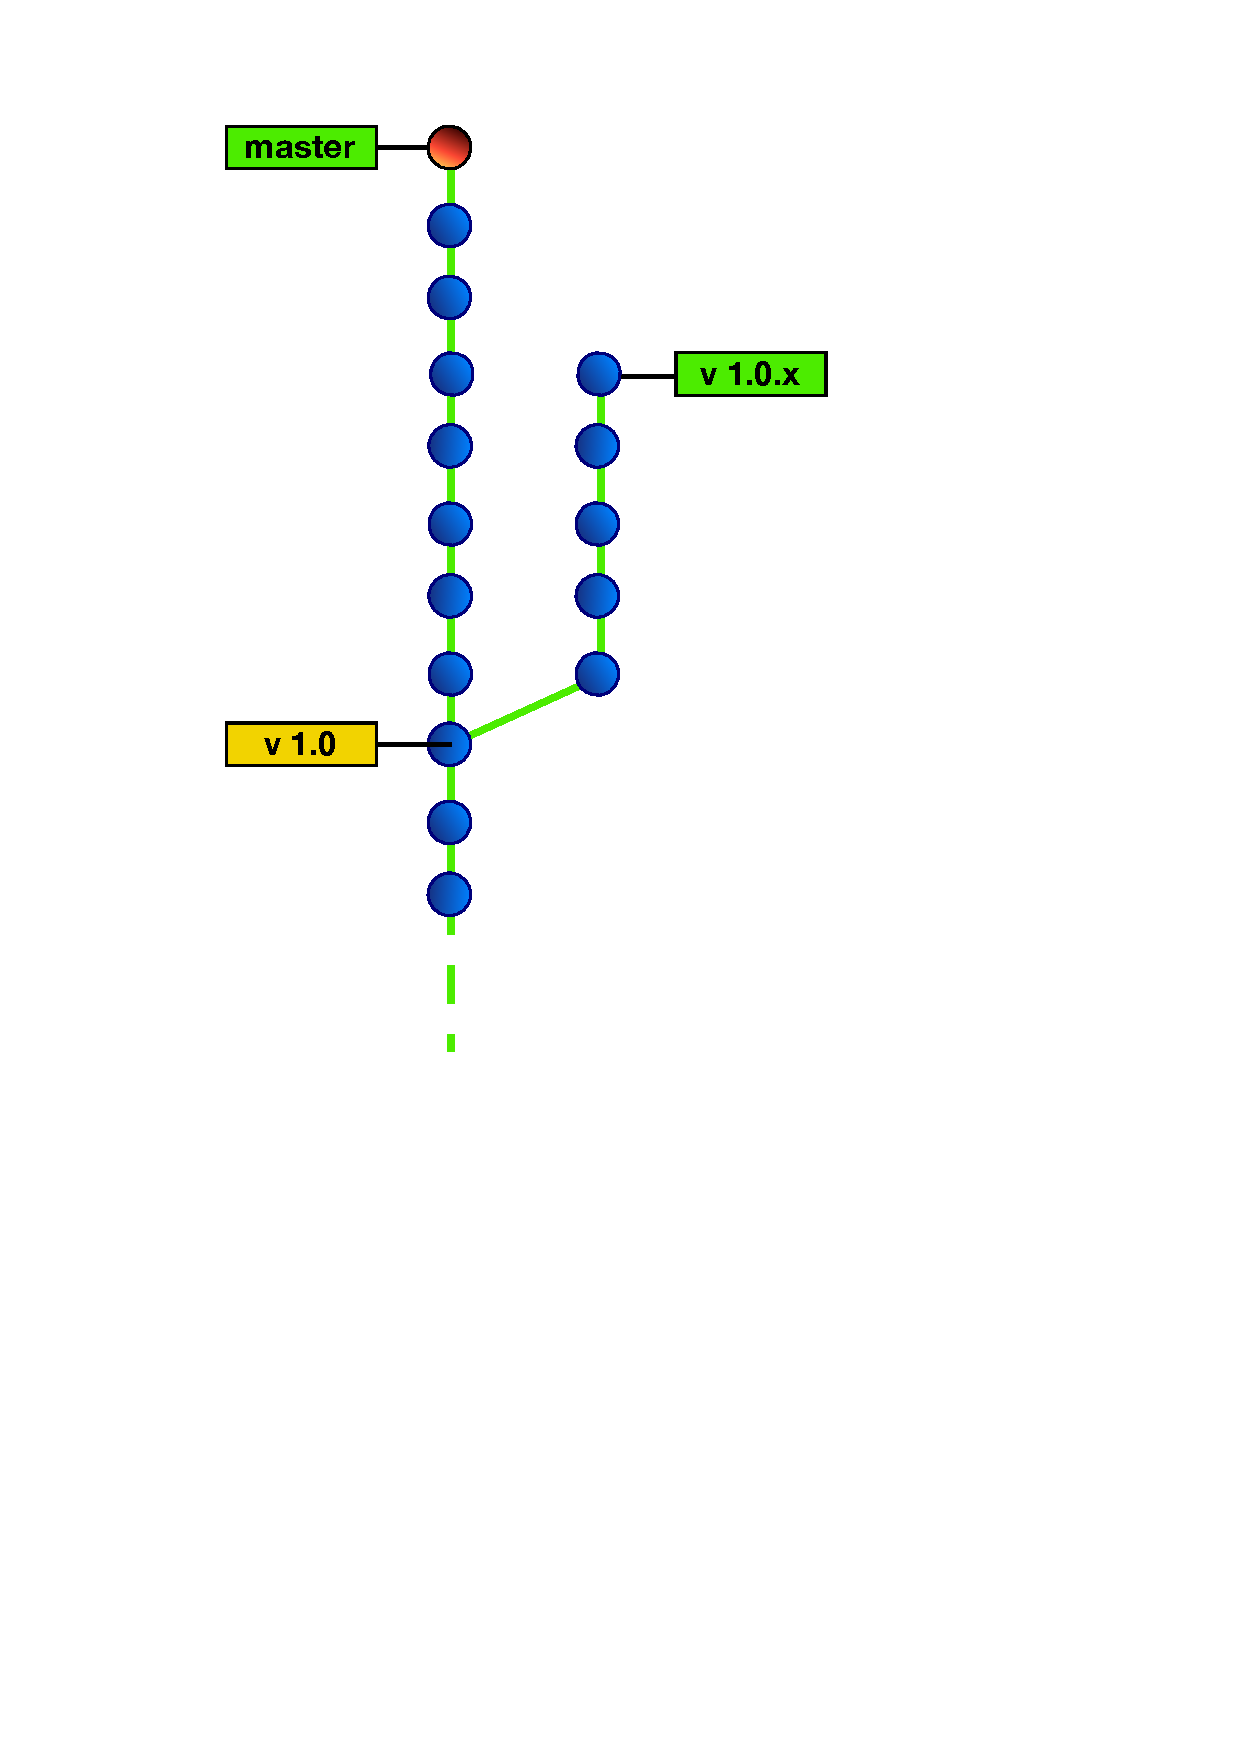
\includegraphics[height=1.5\textwidth]{images/branches.pdf}
\end{column}

\begin{column}{0.60\textwidth}
Une branche

\begin{itemize}
\tightlist
\item
  est une variante de la collection de fichiers
\item
  évolue indépendamment des autres branches
\item
  des opérations de fusion sont possibles
\end{itemize}

Exemples :

\begin{itemize}
\tightlist
\item
  \texttt{master} : branche principale
\item
  \texttt{v1.0.x} : branche de maintenance de la version 1.0
\end{itemize}
\end{column}
\end{columns}

\end{frame}

\begin{frame}[fragile]{%
\protect\hypertarget{illustrations-utilisation-des-branches}{%
Illustrations : utilisation des branches}}

\begin{columns}[T]
\begin{column}{0.40\textwidth}
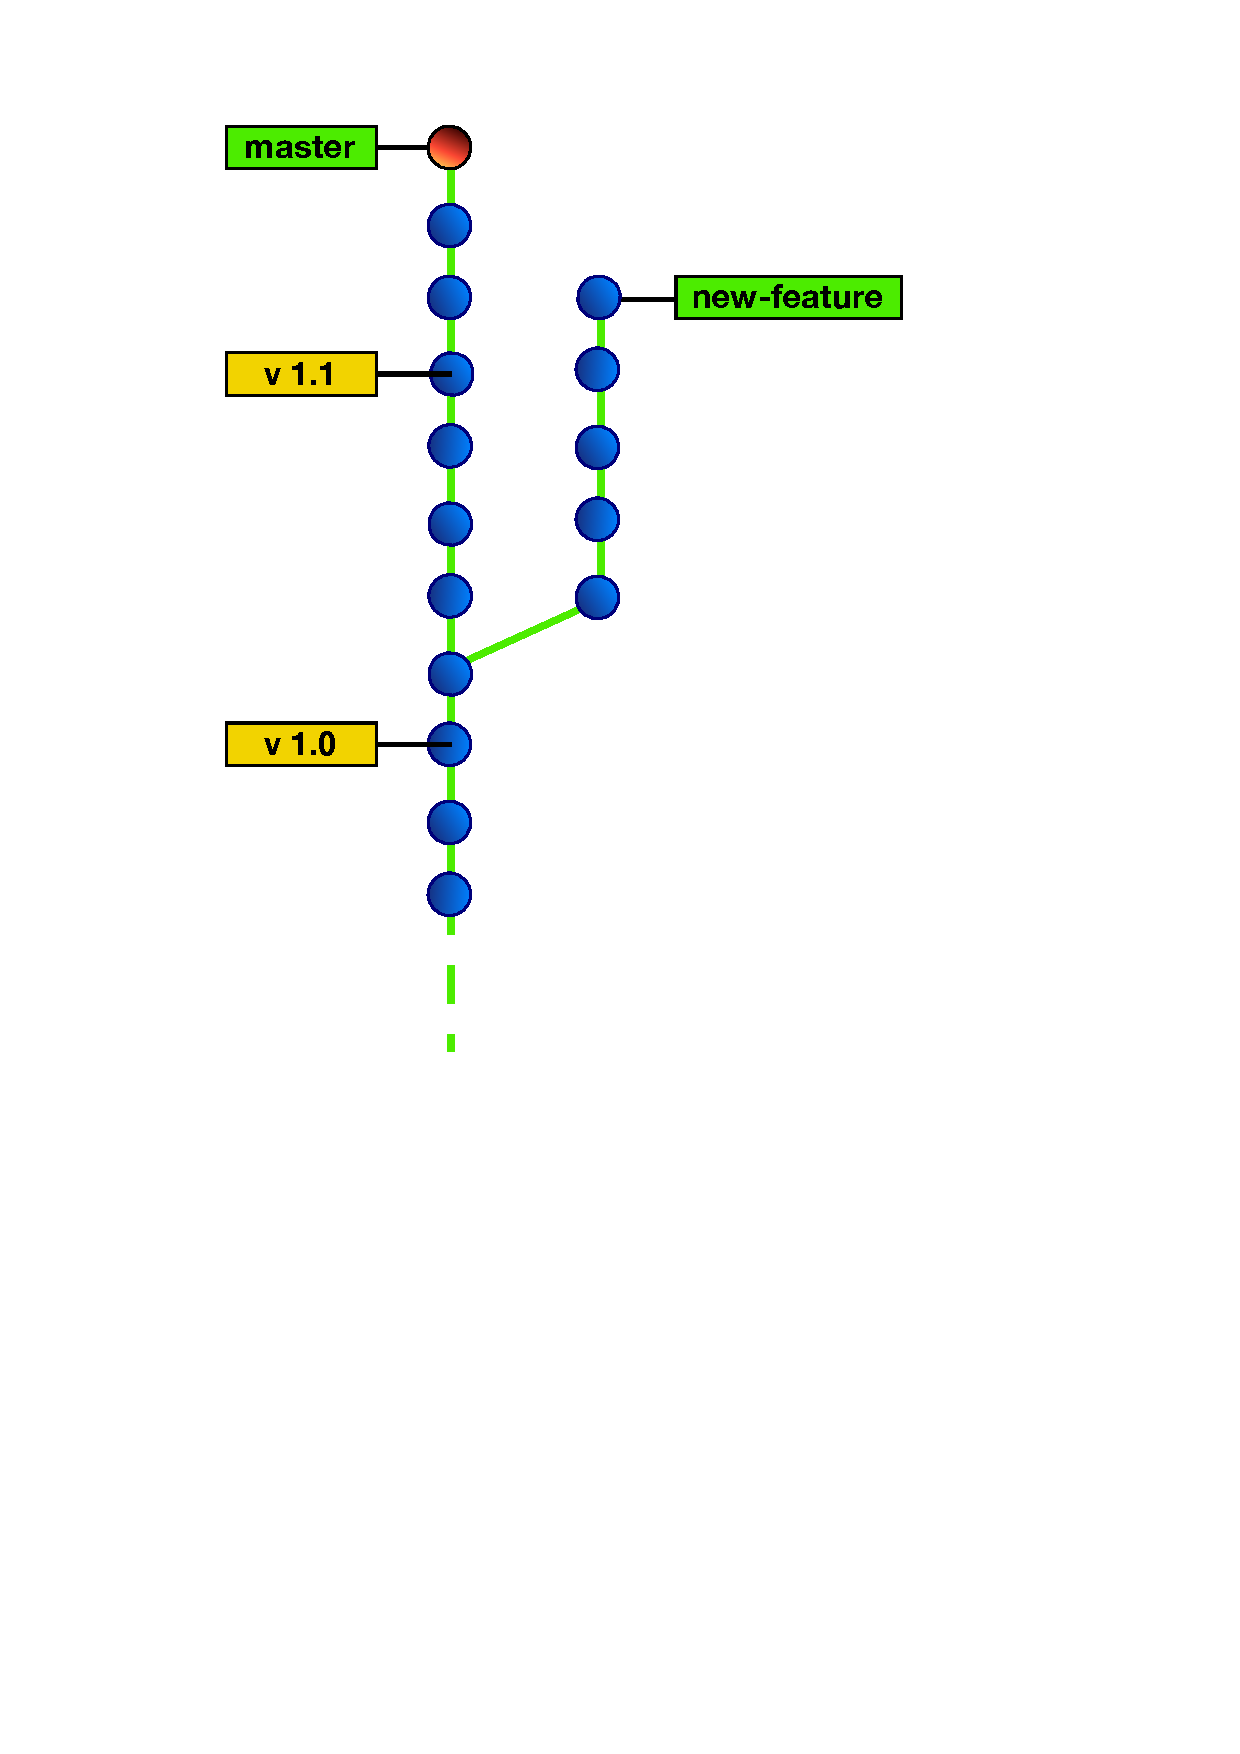
\includegraphics[height=1.5\textwidth]{images/feature.pdf}
\end{column}

\begin{column}{0.60\textwidth}
La branche \texttt{new-feature}permet de

\begin{itemize}
\tightlist
\item
  développer une nouvelle fonctionnalité

  \begin{itemize}
  \tightlist
  \item
    intrusive
  \end{itemize}
\item
  conserver le développement normal

  \begin{itemize}
  \tightlist
  \item
    sans impact sur le processus
  \end{itemize}
\end{itemize}
\end{column}
\end{columns}

\end{frame}

\begin{frame}[fragile]{%
\protect\hypertarget{illustrations-fusion-merge}{%
Illustrations : fusion (merge)}}

\begin{columns}[T]
\begin{column}{0.40\textwidth}
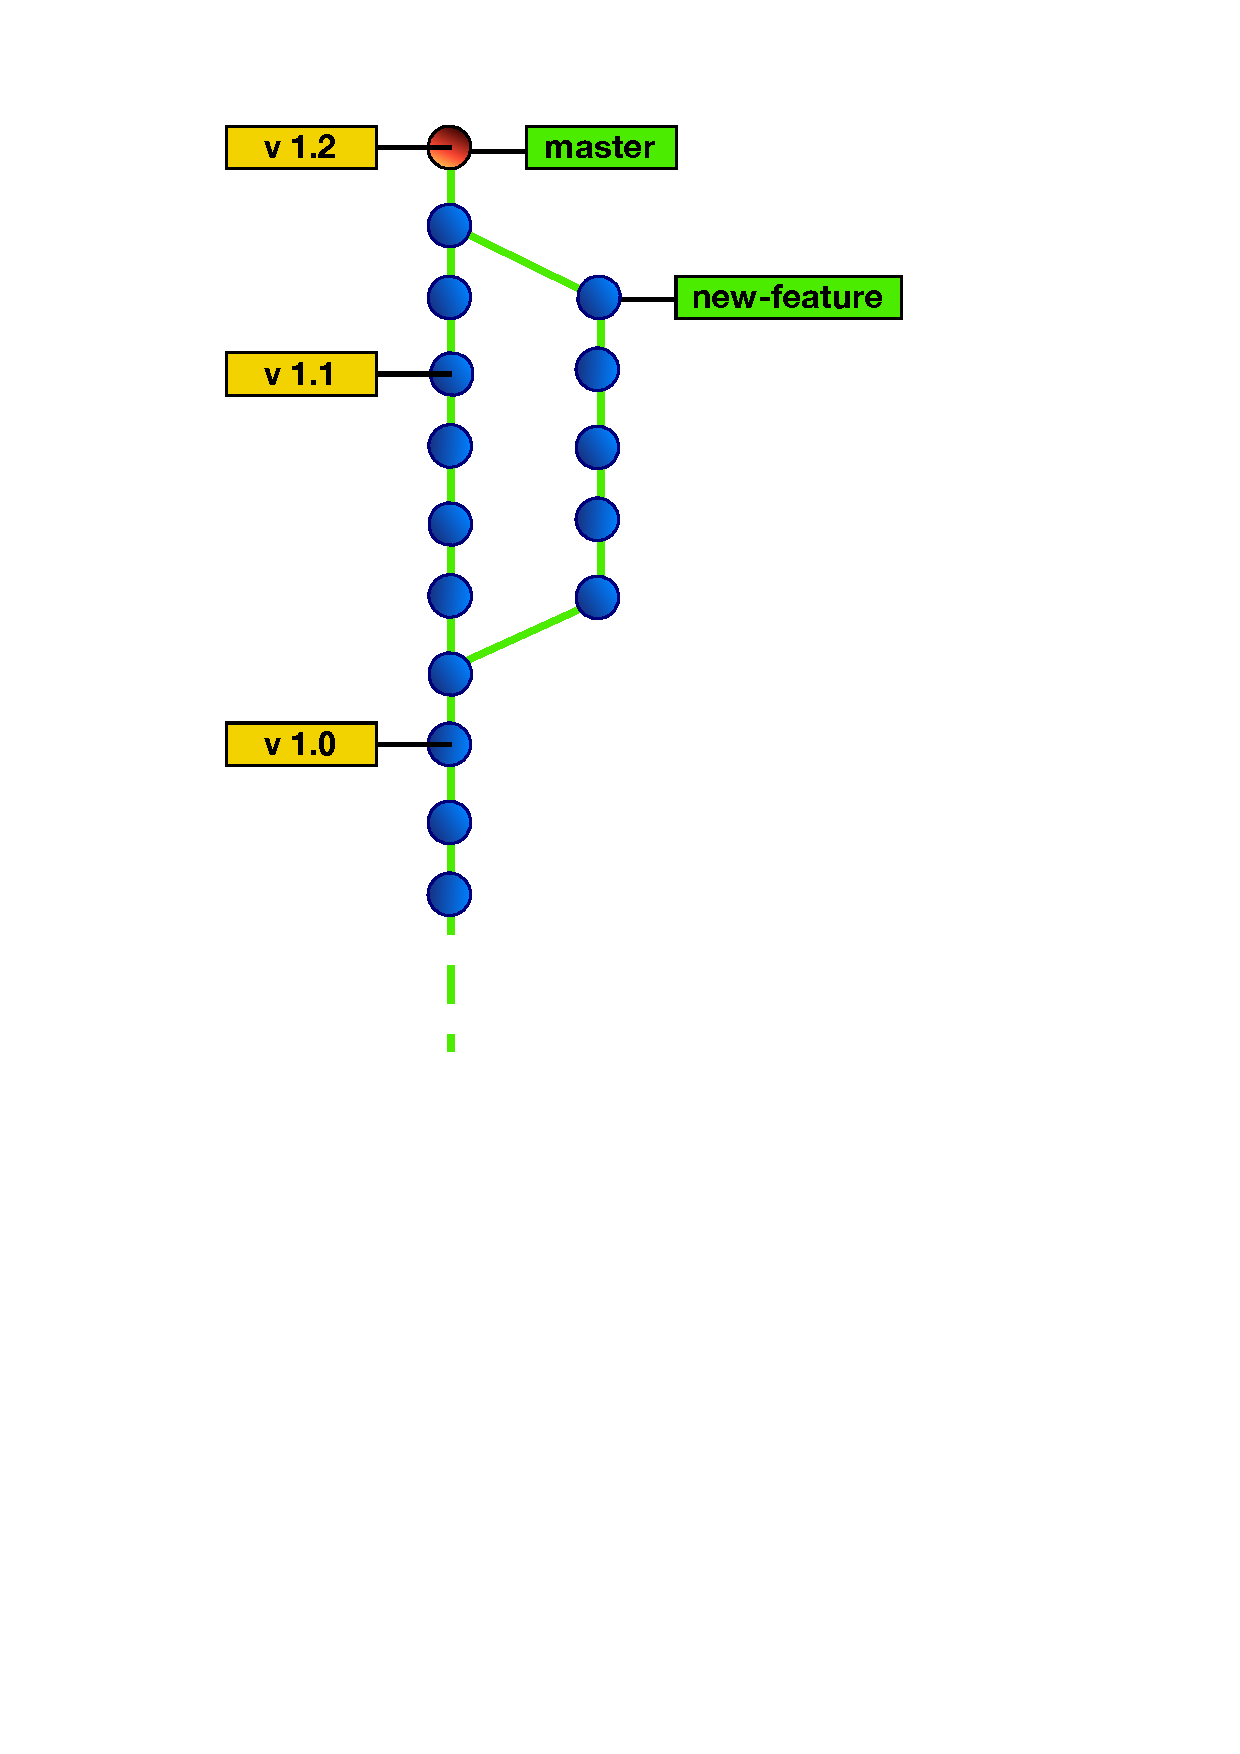
\includegraphics[height=1.5\textwidth]{images/merge.pdf}
\end{column}

\begin{column}{0.60\textwidth}
La branche \texttt{new-feature} est fusionnée à la branche
\texttt{master}

\begin{itemize}
\tightlist
\item
  quand elle est prête
\item
  tous les changements de la branche sont importés
\end{itemize}
\end{column}
\end{columns}

\end{frame}

\begin{frame}{%
\protect\hypertarget{typologie-de-la-gestion-de-versions}{%
Typologie de la gestion de versions}}

\begin{itemize}
\tightlist
\item
  Architecture

  \begin{itemize}
  \tightlist
  \item
    \textbf{centralisée} : tout le monde travaille sur le même
    référentiel
  \item
    \textbf{décentralisée} : chacun a son propre référentiel
  \end{itemize}
\item
  Modèle de concurrence

  \begin{itemize}
  \tightlist
  \item
    \textbf{verrou avant édition} : exclusion mutuelle
  \item
    \textbf{fusion après édition} : gestion des conflits à prévoir
  \end{itemize}
\item
  Gestion de l’historique

  \begin{itemize}
  \tightlist
  \item
    \textbf{arbre} : pas de gestion des fusions
  \item
    \textbf{DAG} : graphe acyclique orienté
  \end{itemize}
\item
  Atomicité

  \begin{itemize}
  \tightlist
  \item
    niveau \textbf{fichier}
  \item
    niveau \textbf{arborescence}
  \end{itemize}
\end{itemize}

\end{frame}

\begin{frame}{%
\protect\hypertarget{interactions-avec-le-repository}{%
Interactions avec le repository}}

\begin{columns}[T]
\begin{column}{0.40\textwidth}
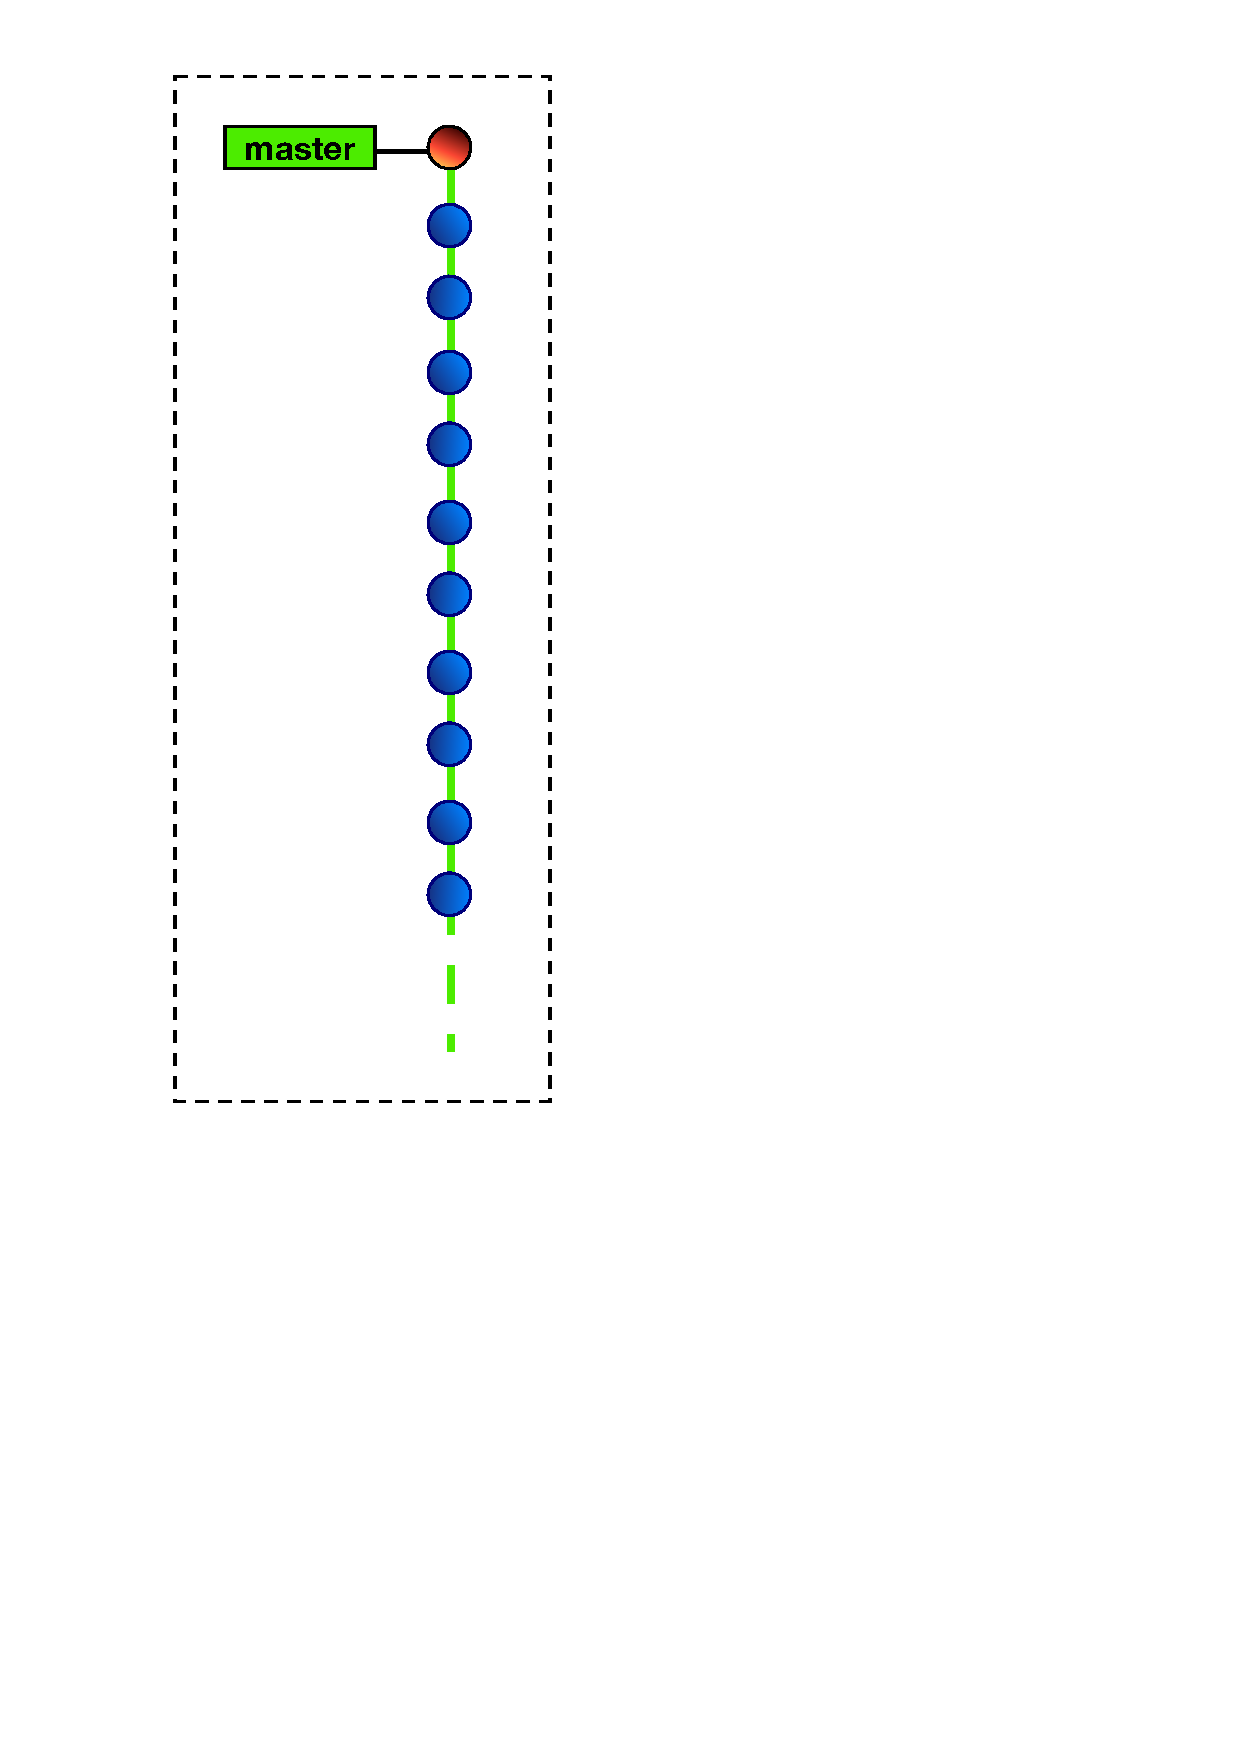
\includegraphics[height=1.5\textwidth]{images/master.pdf}
\end{column}

\begin{column}{0.60\textwidth}
\begin{itemize}
\tightlist
\item
  un référentiel (\emph{repository}) est une entité opaque, pas question
  de l’éditer directement
\item
  On doit extraire sa copie de travail (\emph{working copy}) du
  repository
\end{itemize}
\end{column}
\end{columns}

\end{frame}

\begin{frame}[fragile]{%
\protect\hypertarget{interactions-avec-le-repository-checkout}{%
Interactions avec le repository : \textbf{checkout}}}

\begin{columns}[T]
\begin{column}{0.40\textwidth}
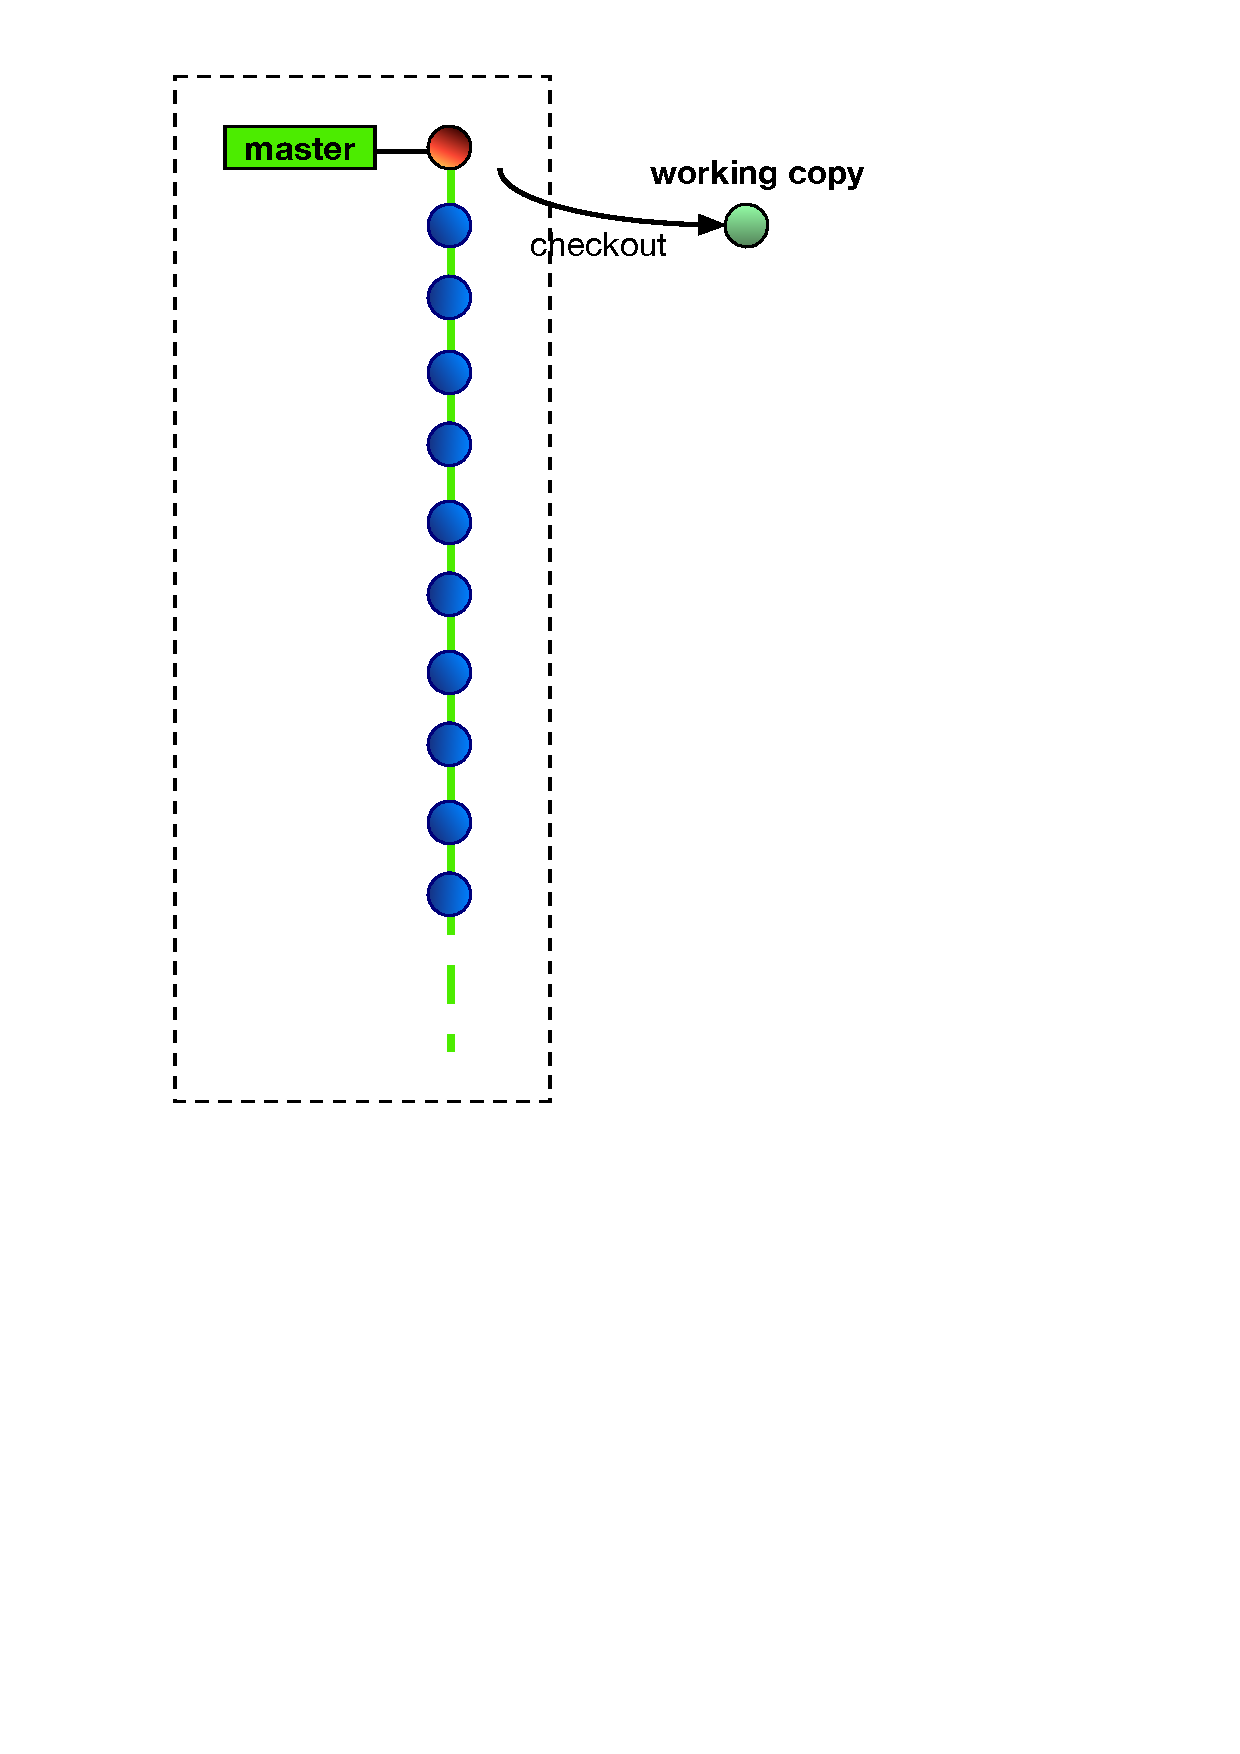
\includegraphics[height=1.5\textwidth]{images/checkout.pdf}
\end{column}

\begin{column}{0.60\textwidth}
\begin{itemize}
\tightlist
\item
  la commande \texttt{checkout} extrait une révision (le plus souvent la
  dernière) du référentiel
\end{itemize}
\end{column}
\end{columns}

\end{frame}

\begin{frame}{%
\protect\hypertarget{interactions-avec-le-repository-uxe9dition}{%
Interactions avec le repository : édition}}

\begin{columns}[T]
\begin{column}{0.40\textwidth}
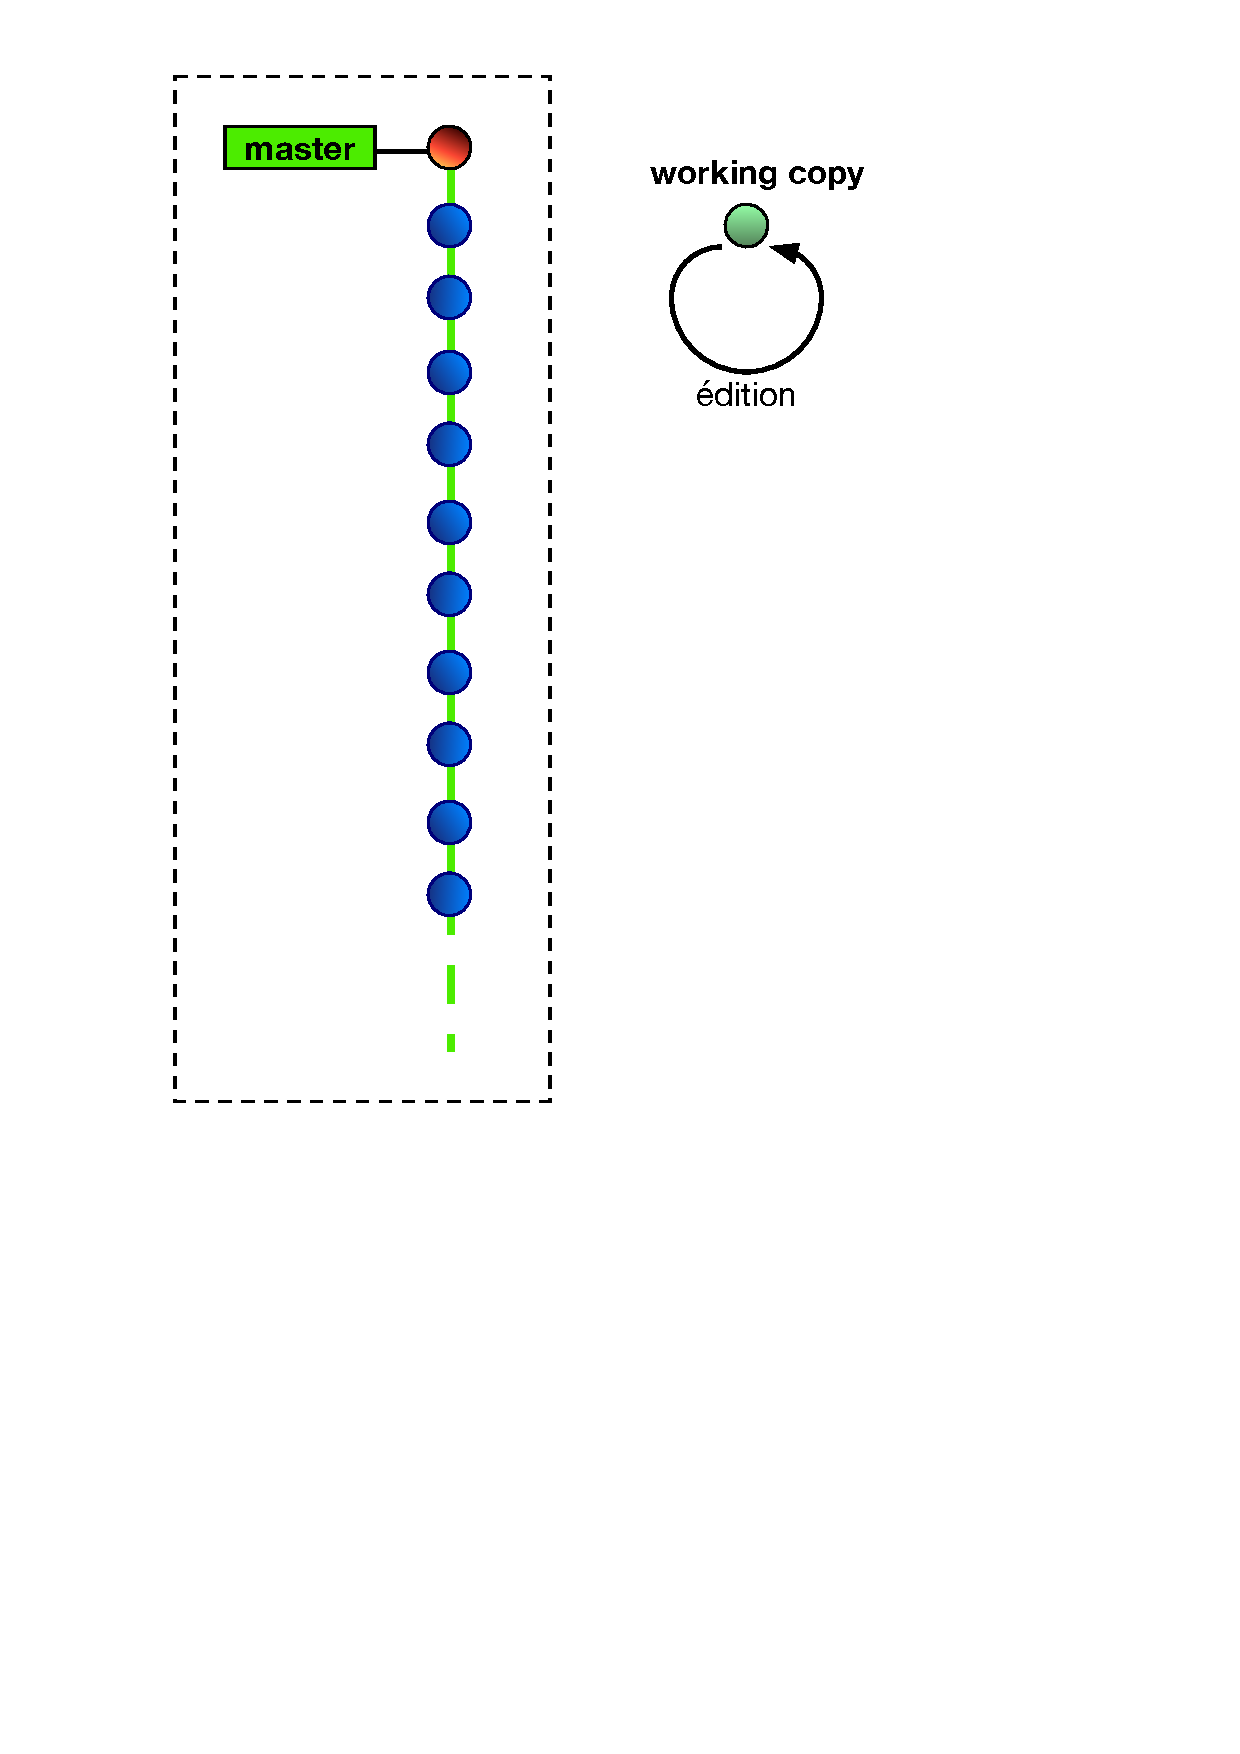
\includegraphics[height=1.5\textwidth]{images/edition.pdf}
\end{column}

\begin{column}{0.60\textwidth}
\begin{itemize}
\tightlist
\item
  la copie de travail est stockée sur le disque local
\item
  elle peut être modifiée, compilée\ldots{}
\end{itemize}
\end{column}
\end{columns}

\end{frame}

\begin{frame}[fragile]{%
\protect\hypertarget{interactions-avec-le-repository-commit}{%
Interactions avec le repository : \textbf{commit}}}

\begin{columns}[T]
\begin{column}{0.40\textwidth}
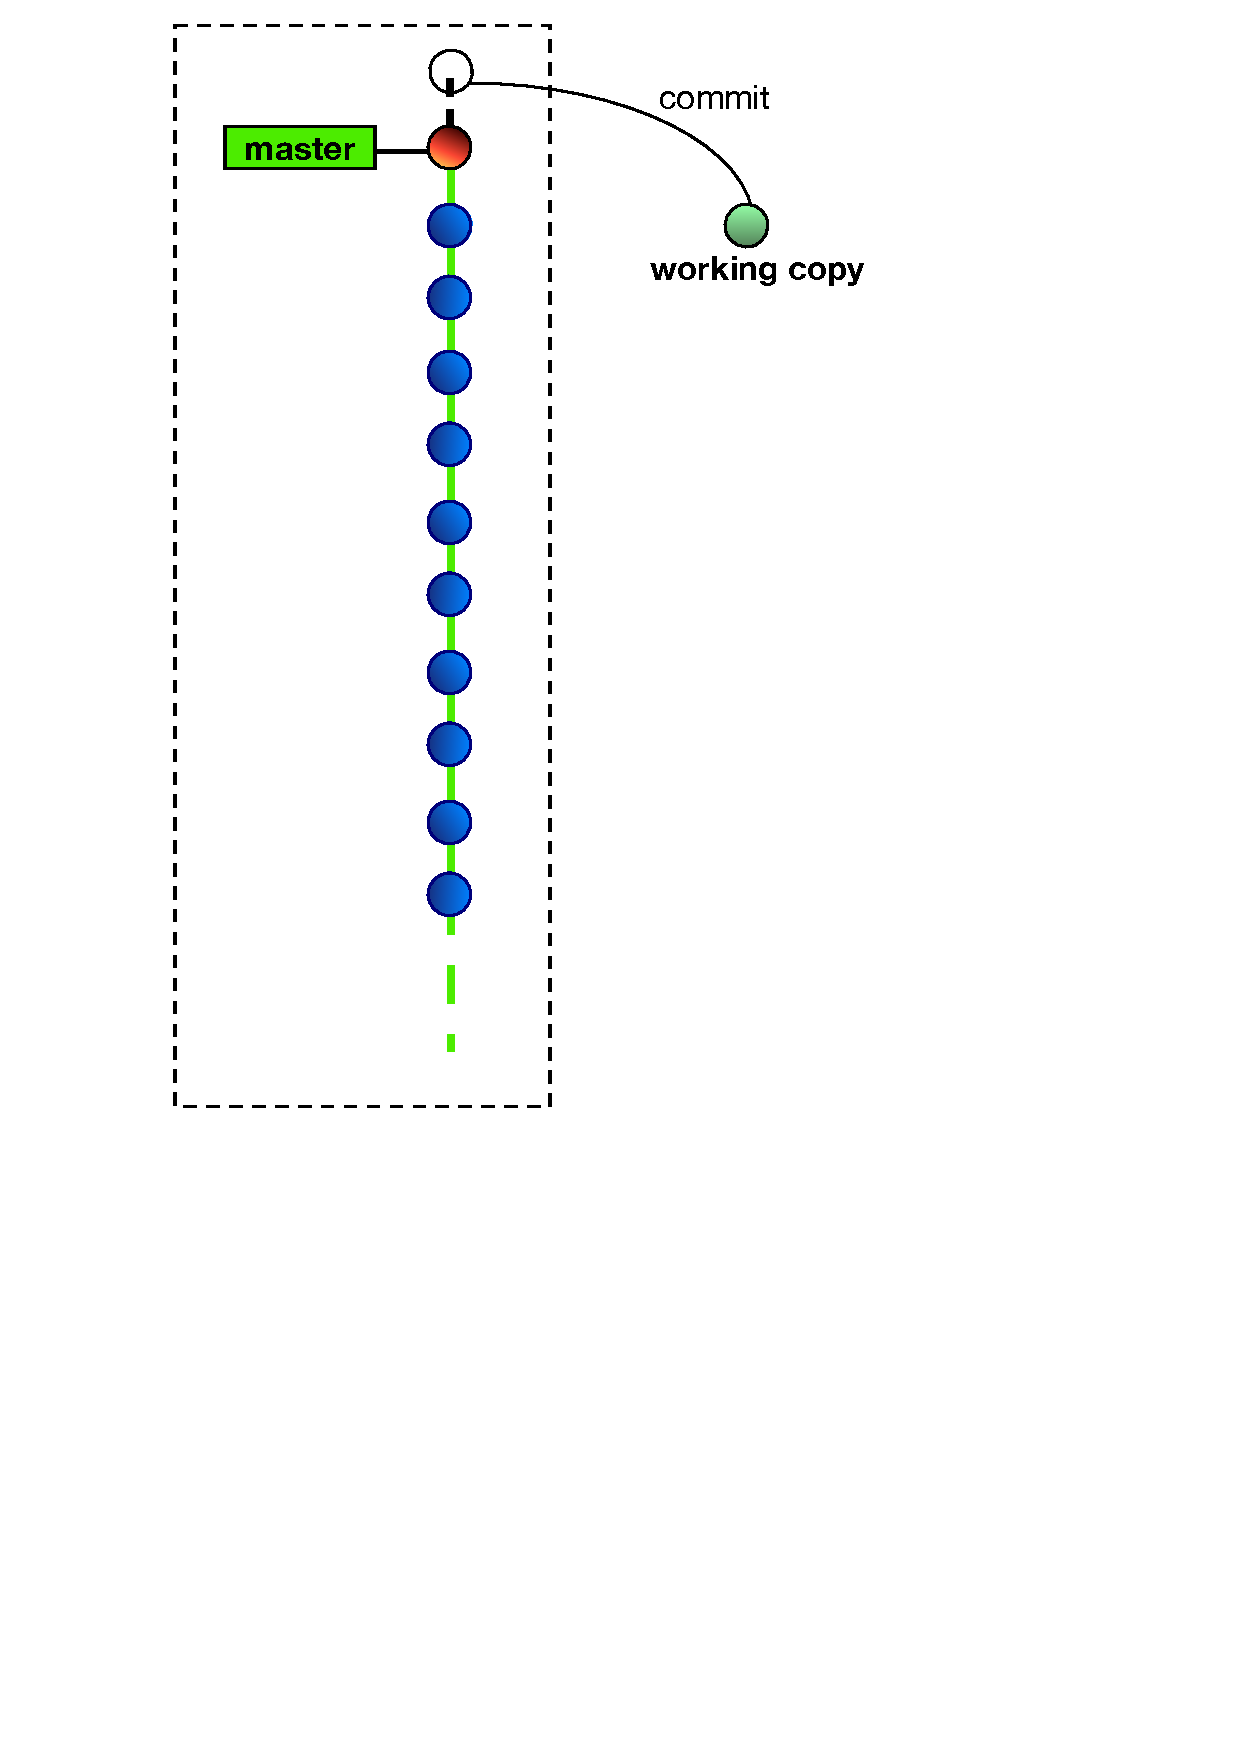
\includegraphics[height=1.5\textwidth]{images/commit.pdf}
\end{column}

\begin{column}{0.60\textwidth}
\begin{itemize}
\tightlist
\item
  la commande \texttt{commit} crée une nouvelle révision à partir de la
  copie de travail
\item
  le processus édition puis \texttt{commit} peut se répéter plusieurs
  fois
\end{itemize}
\end{column}
\end{columns}

\end{frame}

\begin{frame}[fragile]{%
\protect\hypertarget{que-stocke-t-on-dans-le-repository}{%
Que stocke-t-on dans le repository ?}}

\begin{itemize}
\tightlist
\item
  Tous les fichiers qui ne sont \textbf{pas} générés par un outil

  \begin{itemize}
  \tightlist
  \item
    des fichiers sources (\texttt{.c\ .cpp\ .java\ .tex\ .sql})
  \item
    des scripts de build, des fichiers de projets
    (\texttt{Makefile\ CMakefile.txt\ ant.xml})
  \item
    des fichiers de documentation (\texttt{.txt\ README})
  \item
    des fichiers de ressources (images, audio\ldots{})
  \end{itemize}
\item
  Il ne faut pas stocker les fichiers générés (sous peine de gérer des
  confluts inutiles)

  \begin{itemize}
  \tightlist
  \item
    \texttt{.o\ .obj\ .a\ .lib\ .so\ .dll\ .class\ .jar\ .exe}\ldots{}
  \item
    les scripts de build quand ils sont générés par un autre outil

    \begin{itemize}
    \tightlist
    \item
      exemple : \texttt{cmake} qui génère des \texttt{Makefile}
    \end{itemize}
  \end{itemize}
\end{itemize}

\end{frame}

\begin{frame}[fragile]{%
\protect\hypertarget{quelques-bonnes-pratiques-de-commit}{%
Quelques bonnes pratiques de \texttt{commit}}}

\begin{itemize}
\tightlist
\item
  Faire des \texttt{commit} \textbf{souvent}
\item
  Faire des \texttt{commit} relatifs à des changements indépendants dans
  des révisions différentes
\item
  Ecrire des messages de \texttt{commit}

  \begin{itemize}
  \tightlist
  \item
    c’est obligatoire !
  \item
    décrire le pourquoi du changement plutôt que le changement lui-même
  \end{itemize}
\end{itemize}

\end{frame}

\begin{frame}{%
\protect\hypertarget{un-peu-dhistoire-de-la-gestion-de-version-centralisuxe9e}{%
Un peu d’histoire de la gestion de version centralisée}}

\begin{itemize}
\tightlist
\item
  1ère génération (mono fichier, utilisation locale, exclusion mutuelle)

  \begin{itemize}
  \tightlist
  \item
    1972 : SCCS
  \item
    1982 : RCS
  \item
    1985 : PVCS
  \end{itemize}
\item
  2ème génération (multi-fichiers, client-serveur, fusion après commit)

  \begin{itemize}
  \tightlist
  \item
    1986 : CVS
  \item
    1992 : Rational ClearCase
  \item
    1994 : Visual SourceSafe
  \end{itemize}
\item
  3ème génération (2ème + atomicité)

  \begin{itemize}
  \tightlist
  \item
    1995 : Perforce
  \item
    2000 : \textbf{subversion}
  \item
    plein d’autres\ldots{}
  \end{itemize}
\end{itemize}

\end{frame}

\begin{frame}{%
\protect\hypertarget{gestion-de-version-duxe9centralisuxe9e}{%
Gestion de version décentralisée}}

\begin{itemize}
\tightlist
\item
  les prémisses au début des années 2000

  \begin{itemize}
  \tightlist
  \item
    Bitkeeper, GNU Arch
  \end{itemize}
\item
  les outils actuels (2005)

  \begin{itemize}
  \tightlist
  \item
    Bazaar
  \item
    Mercurial
  \item
    git
  \end{itemize}
\item
  tendance à l’intégration

  \begin{itemize}
  \tightlist
  \item
    gestion de version + gestion des bugs et du projet
  \item
    github, gitlab, bitbucket
  \item
    fossil
  \end{itemize}
\end{itemize}

\end{frame}

\hypertarget{utilisation-de-git-en-local}{%
\section{Utilisation de git en
local}\label{utilisation-de-git-en-local}}

\begin{frame}[fragile]{%
\protect\hypertarget{histoire}{%
Histoire}}

\begin{itemize}
\tightlist
\item
  Avant 2005 : les sources de Linux étaient gérées avec Bitkeeper, outil
  propriétaire
\item
  Avril 2005 : révocation de la licence de libre utilisation
\item
  Rien d’autre dans le paysage en termes de maturité

  \begin{itemize}
  \tightlist
  \item
    Linus Torvald a commencé à développer \texttt{git}
  \end{itemize}
\item
  Juin 2005 : première version de Linux gérée avec \texttt{git}
\item
  Décembre 2005 : sortie de \texttt{git}1.0
\end{itemize}

\end{frame}

\begin{frame}{%
\protect\hypertarget{utilisation-de-git}{%
Utilisation de git}}

\begin{columns}[T]
\begin{column}{0.40\textwidth}
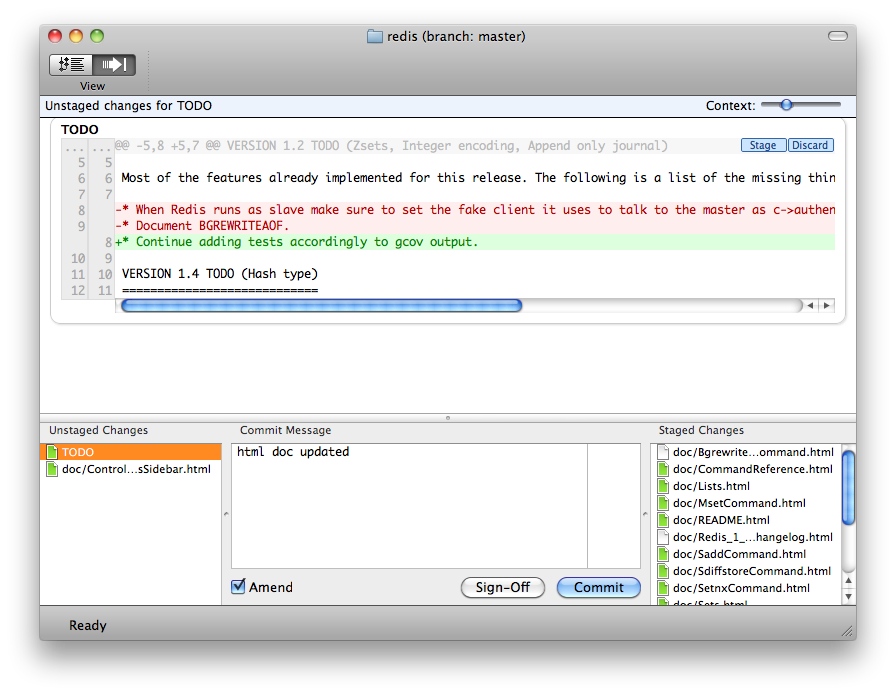
\includegraphics[width=1\textwidth]{images/GitX-Commit.png}

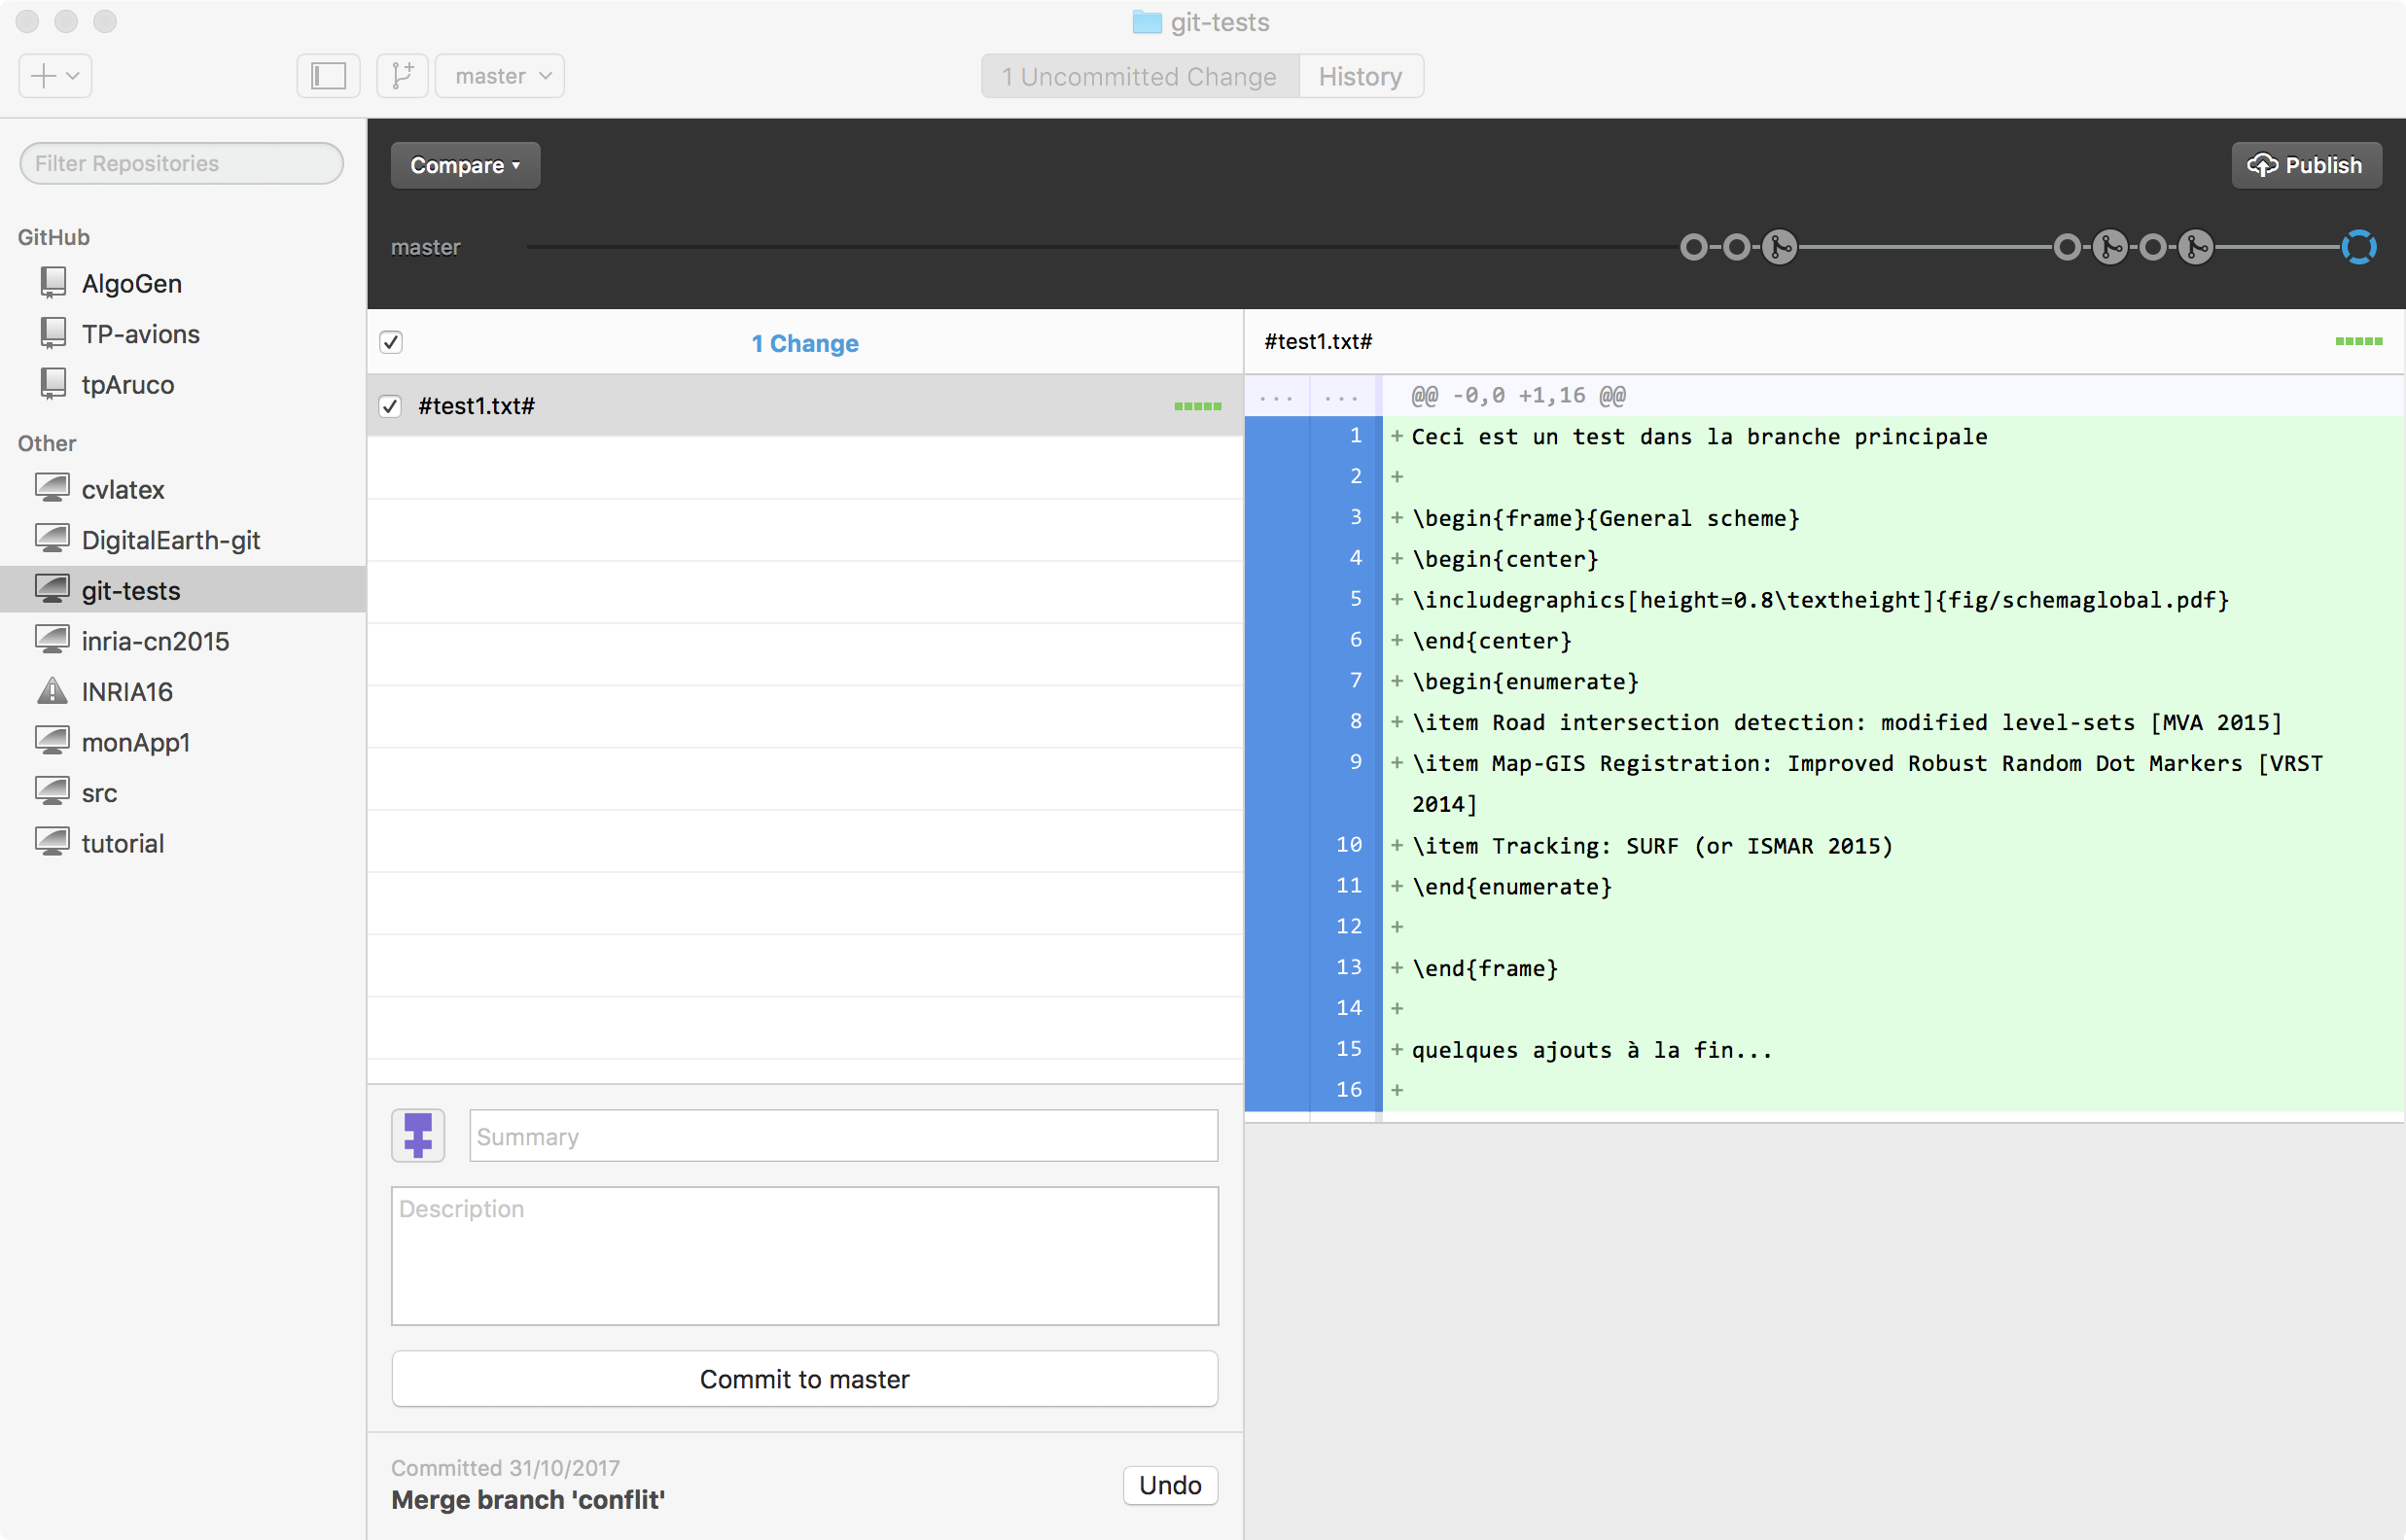
\includegraphics[width=1\textwidth]{images/github.png}
\end{column}

\begin{column}{0.60\textwidth}
\begin{itemize}
\tightlist
\item
  la ligne de commande (installé par défaut avec les autres outils ou
  certains IDE)
\item
  Turtoise Git (Windows)
\item
  Github (toutes plate-formes)
\item
  plugins git (Eclipse, Netbeans, Atom\ldots{})
\end{itemize}
\end{column}
\end{columns}

\end{frame}

\begin{frame}[fragile]{%
\protect\hypertarget{cruxe9ation-dun-ruxe9fuxe9rentiel-local}{%
Création d’un référentiel local}}

\begin{verbatim}
git init myrepository
\end{verbatim}

Cette commande crée un répertoire \emph{myrepository} * le repository
lui même est contenu dans \emph{myrepository/.git} * une copie de
travail (initialement vide) est créée dans \emph{myrepository/}

\begin{verbatim}
[MbP-GM15:~/tmp] moreau% pwd
/Users/moreau/tmp
[MbP-GM15:~/tmp] moreau% git init helloworld
Initialized empty Git repository in /Users/moreau/tmp/helloworld/.git/
[MbP-GM15:~/tmp] moreau% ls -a helloworld/
.    ..   .git
[MbP-GM15:~/tmp] moreau% ls -a helloworld/.git
.           HEAD        config      hooks       objects
..          branches    description info        refs
\end{verbatim}

\end{frame}

\begin{frame}[fragile]{%
\protect\hypertarget{premiers-commits}{%
Premiers commits}}

\begin{verbatim}
git add file
git commit [-m message]
\end{verbatim}

Avec \texttt{git}, il y a deux opérations :

\begin{itemize}
\tightlist
\item
  add
\item
  commit
\end{itemize}

Par défaut les commits sont effectués dans la branche \emph{master}

\end{frame}

\begin{frame}[fragile]{%
\protect\hypertarget{exemple}{%
Exemple}}

\begin{verbatim}
[MbP-GM15:~/tmp] moreau% cd helloworld/
[MbP-GM15:~/tmp/helloworld] moreau% emacs hello.txt
[MbP-GM15:~/tmp/helloworld] moreau% git add hello.txt
[MbP-GM15:~/tmp/helloworld] moreau% git commit -m "ajout du fichier hello.txt"
[master (root-commit) b9e1f92] ajout du fichier hello.txt
 1 file changed, 1 insertion(+)
 create mode 100644 hello.txt
[MbP-GM15:~/tmp/helloworld] moreau%
\end{verbatim}

Remarque : git utilise des hash \texttt{b9e1f92} pour numéroter les
commits

\end{frame}

\begin{frame}[fragile]{%
\protect\hypertarget{lindex-staging-area}{%
L’index (staging area)}}

Les systèmes de gestion de version utilisent deux espaces :

\begin{itemize}
\tightlist
\item
  le référentiel

  \begin{itemize}
  \tightlist
  \item
    toute l’histoire de votre projet
  \end{itemize}
\item
  la copie de travail

  \begin{itemize}
  \tightlist
  \item
    les fichiers que vous éditez et qui feront partie du prochain commit
  \end{itemize}
\end{itemize}

\texttt{git} introduit un espace intermédiaire : la \textbf{staging
area} parfois appelée \textbf{index} qui stocke les fichiers en vue du
prochain commit\footnote<.->{la motivation et l’utilisation sortent du
  cadre de ce cours} :

\begin{itemize}
\tightlist
\item
  \texttt{git\ add} \emph{files} copie les fichiers vers l’index
\item
  \texttt{git\ commit} effectue le commit du contenu de l’index
\end{itemize}

\end{frame}

\begin{frame}[fragile]{%
\protect\hypertarget{exemple-modification-dun-fichier}{%
Exemple : modification d’un fichier}}

\begin{verbatim}
[MbP-GM15:~/tmp/helloworld] moreau% echo 'bla bla bla' >> hello.txt
[MbP-GM15:~/tmp/helloworld] moreau% git commit
On branch master
Changes not staged for commit:
    modified:   hello.txt

no changes added to commit
\end{verbatim}

\texttt{git} se plaint qu’il y a rien de changé. En réalité, il faut
faire

\begin{verbatim}
[MbP-GM15:~/tmp/helloworld] moreau% git add hello.txt
[MbP-GM15:~/tmp/helloworld] moreau% git commit -m "quelques changements"
[master 543461a] quelques changements
 1 file changed, 1 insertion(+)
\end{verbatim}

\end{frame}

\begin{frame}{%
\protect\hypertarget{illustration-avec-github}{%
Illustration avec github}}

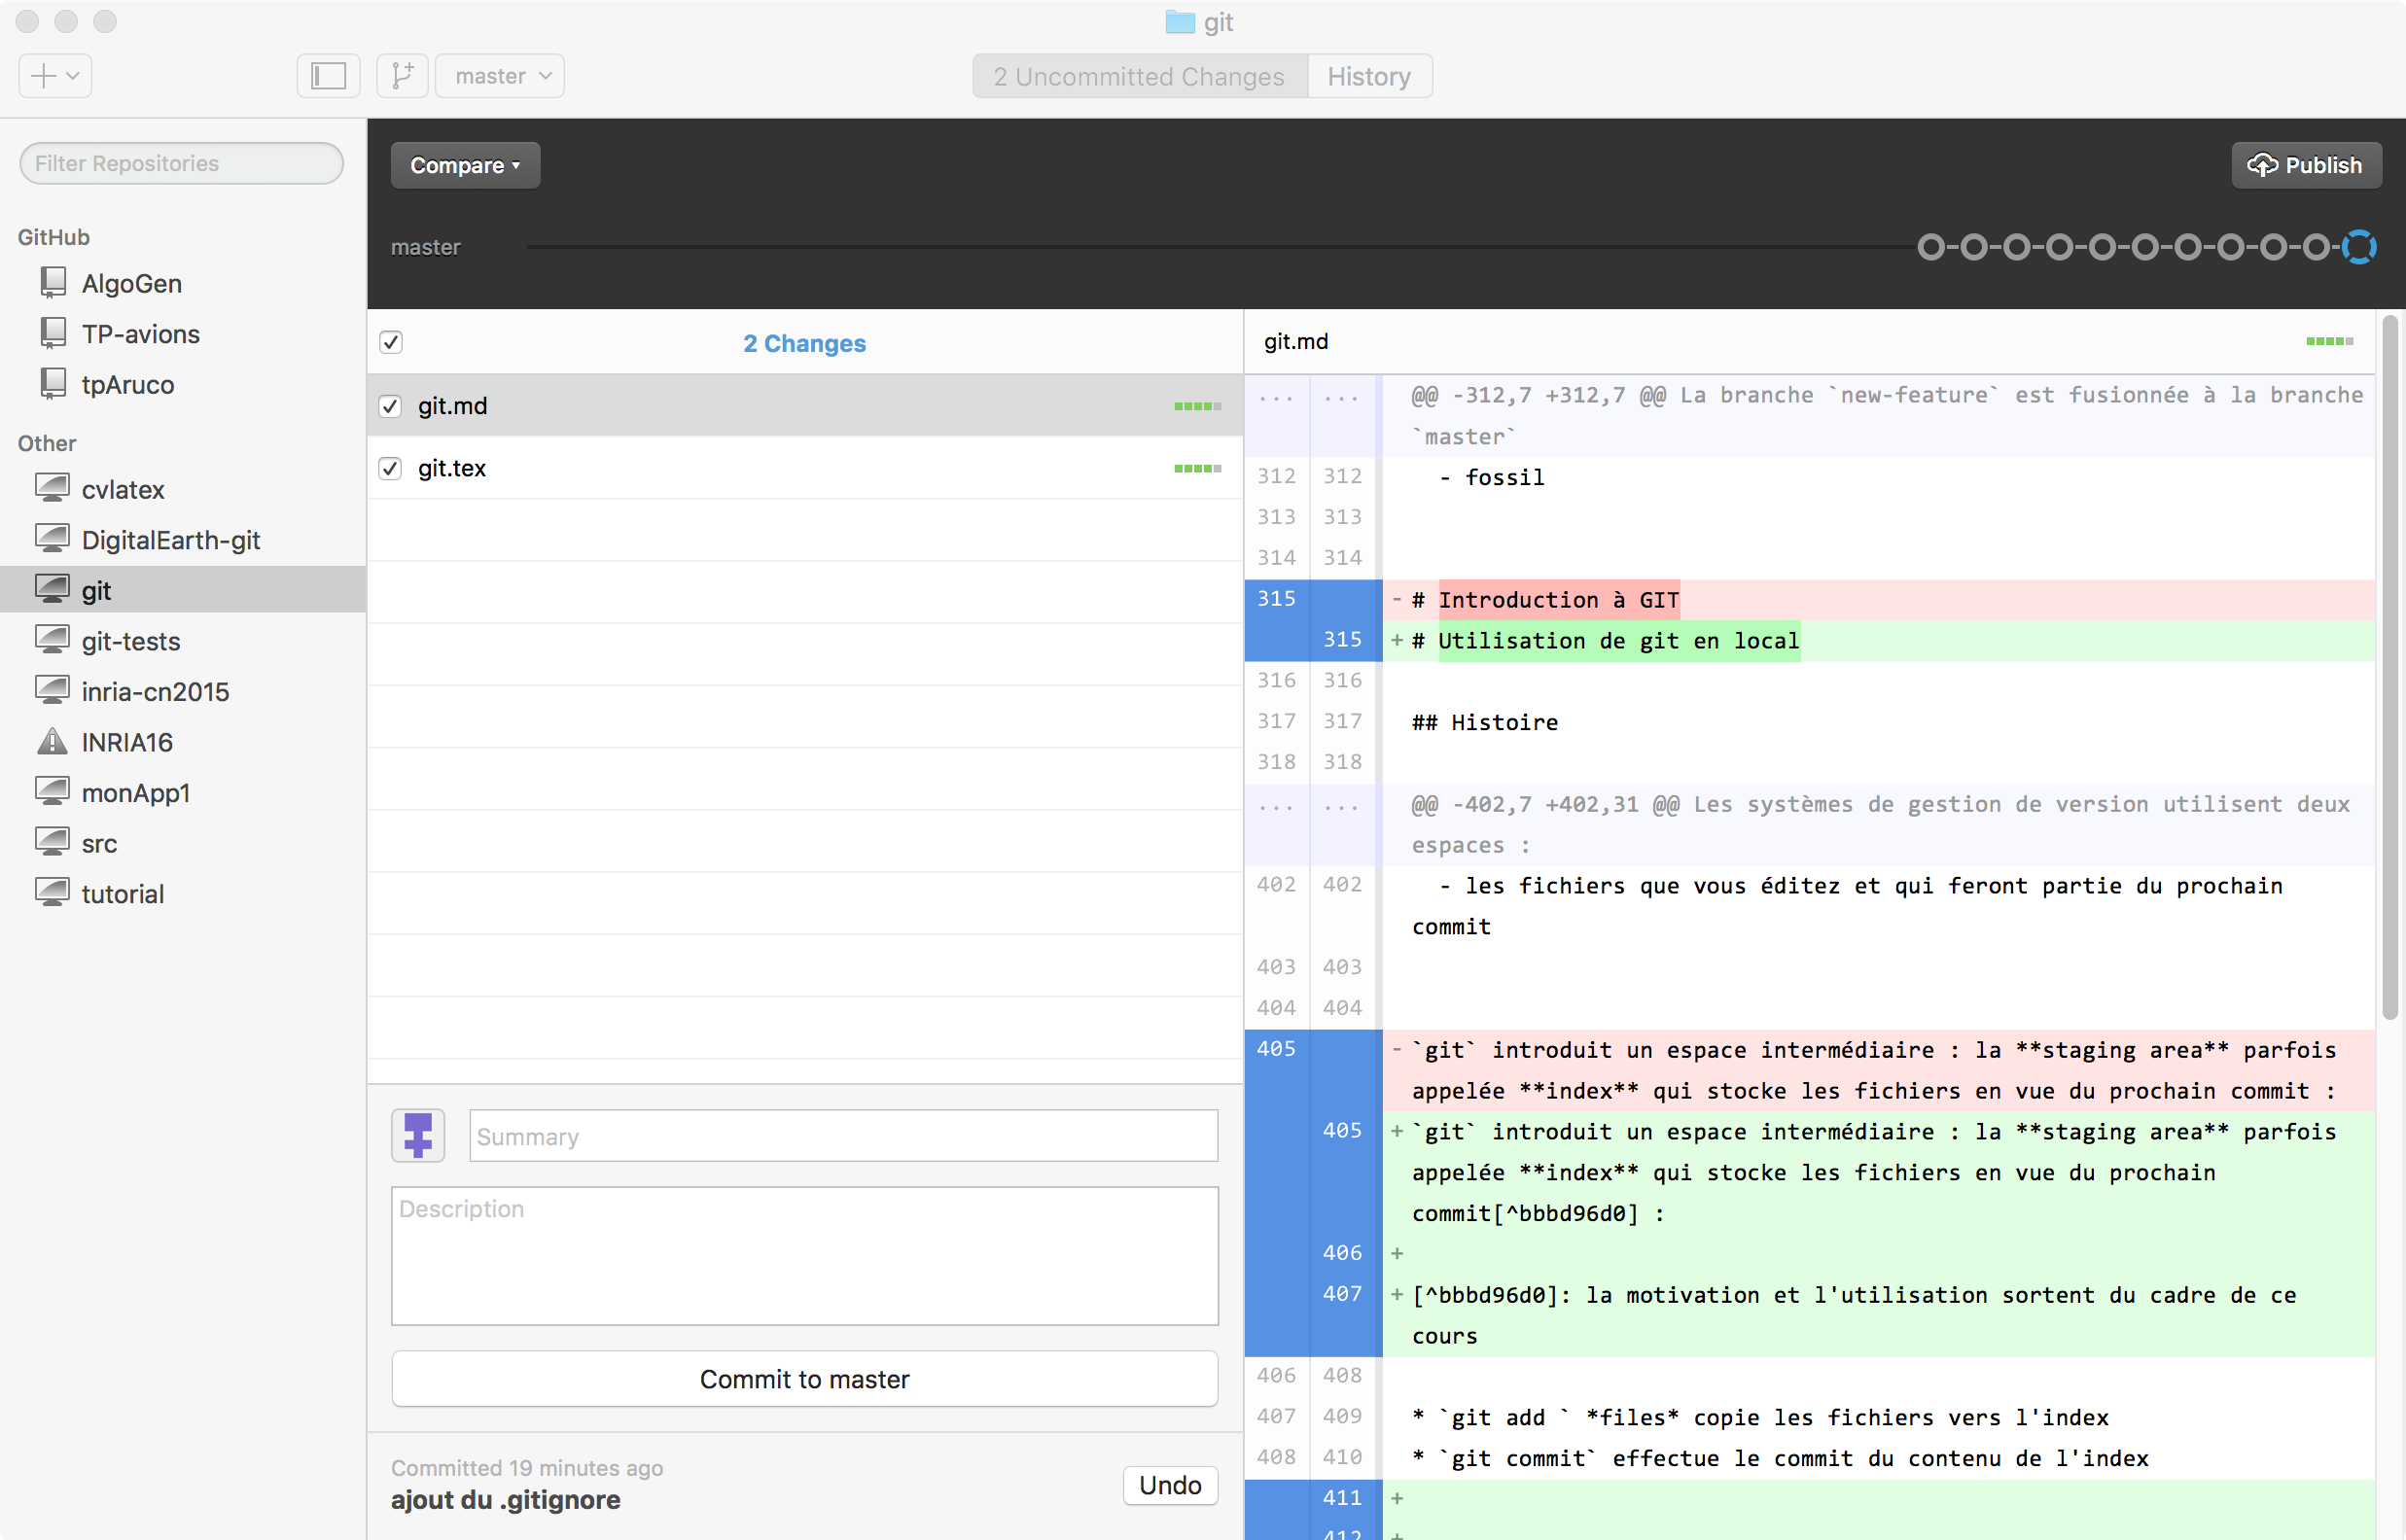
\includegraphics[width=1\textwidth]{images/github-commit.png}

\end{frame}

\begin{frame}{%
\protect\hypertarget{illustration-avec-atom}{%
Illustration avec Atom}}

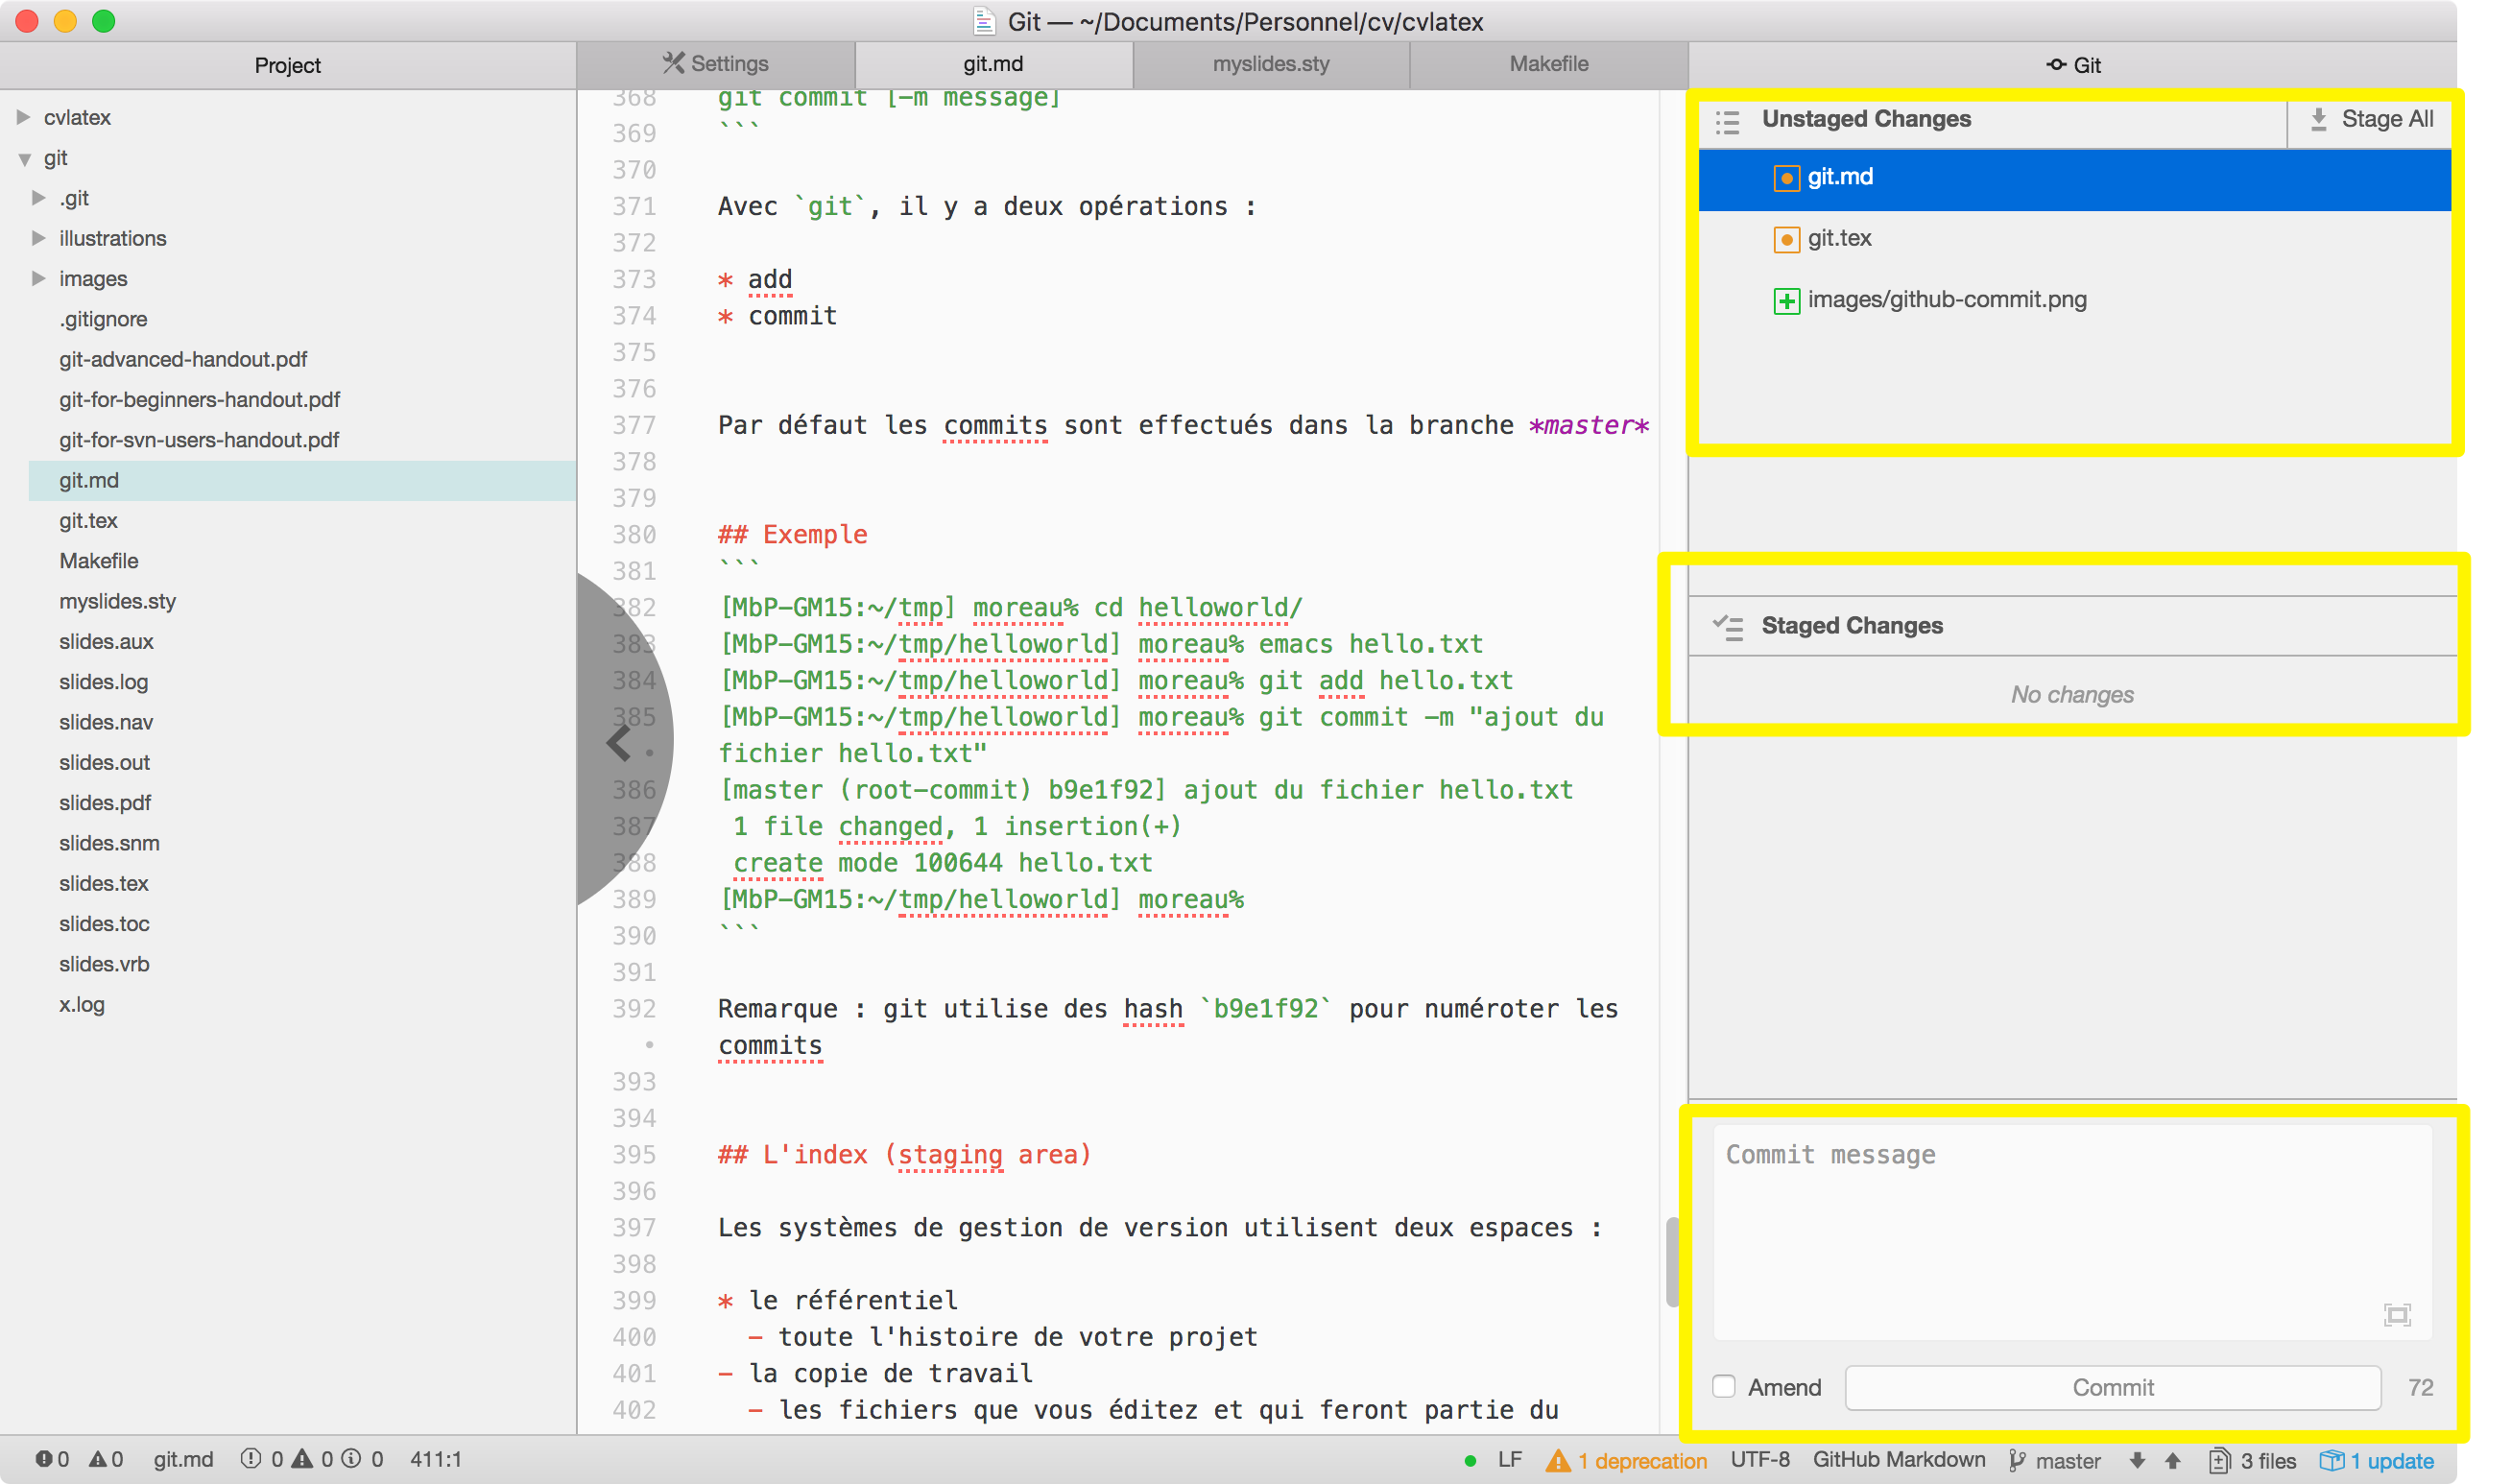
\includegraphics[width=1\textwidth]{images/atom-commit.png}

\end{frame}

\begin{frame}[fragile]{%
\protect\hypertarget{suppression-de-fichiers}{%
Suppression de fichiers}}

\begin{verbatim}
git rm file
git commit
\end{verbatim}

supprime un fichier de la copie de travail et du référentiel

\begin{verbatim}
[MbP-GM15:~/tmp/helloworld] moreau% git rm hello.txt
rm 'hello.txt'
[MbP-GM15:~/tmp/helloworld] moreau% git commit -m "plus besoin"
[master 388f711] plus besoin
 1 file changed, 2 deletions(-)
 delete mode 100644 hello.txt
\end{verbatim}

\end{frame}

\begin{frame}[fragile]{%
\protect\hypertarget{diffuxe9rences-entre-versions}{%
Différences entre versions}}

\begin{verbatim}
git diff [rev_a [rev _b] ]
\end{verbatim}

montre les différences entre 2 révisions \texttt{rev\_a} et
\texttt{rev\_b}

\textbf{Attention}, par défaut :

\begin{itemize}
\tightlist
\item
  \texttt{rev\_a} est l’index
\item
  \texttt{rev\_b} est la copie de travail
\end{itemize}

Si on veut savoir où l’on en est par rapport au référentiel :

\begin{verbatim}
git diff HEAD
git diff master
\end{verbatim}

\end{frame}

\begin{frame}{%
\protect\hypertarget{visualisation-des-diffuxe9rences-entre-versions}{%
Visualisation des différences entre versions}}

Les outils intégrés prennent ici tout leur sens : exemples avec la ligne
de commande et Atom

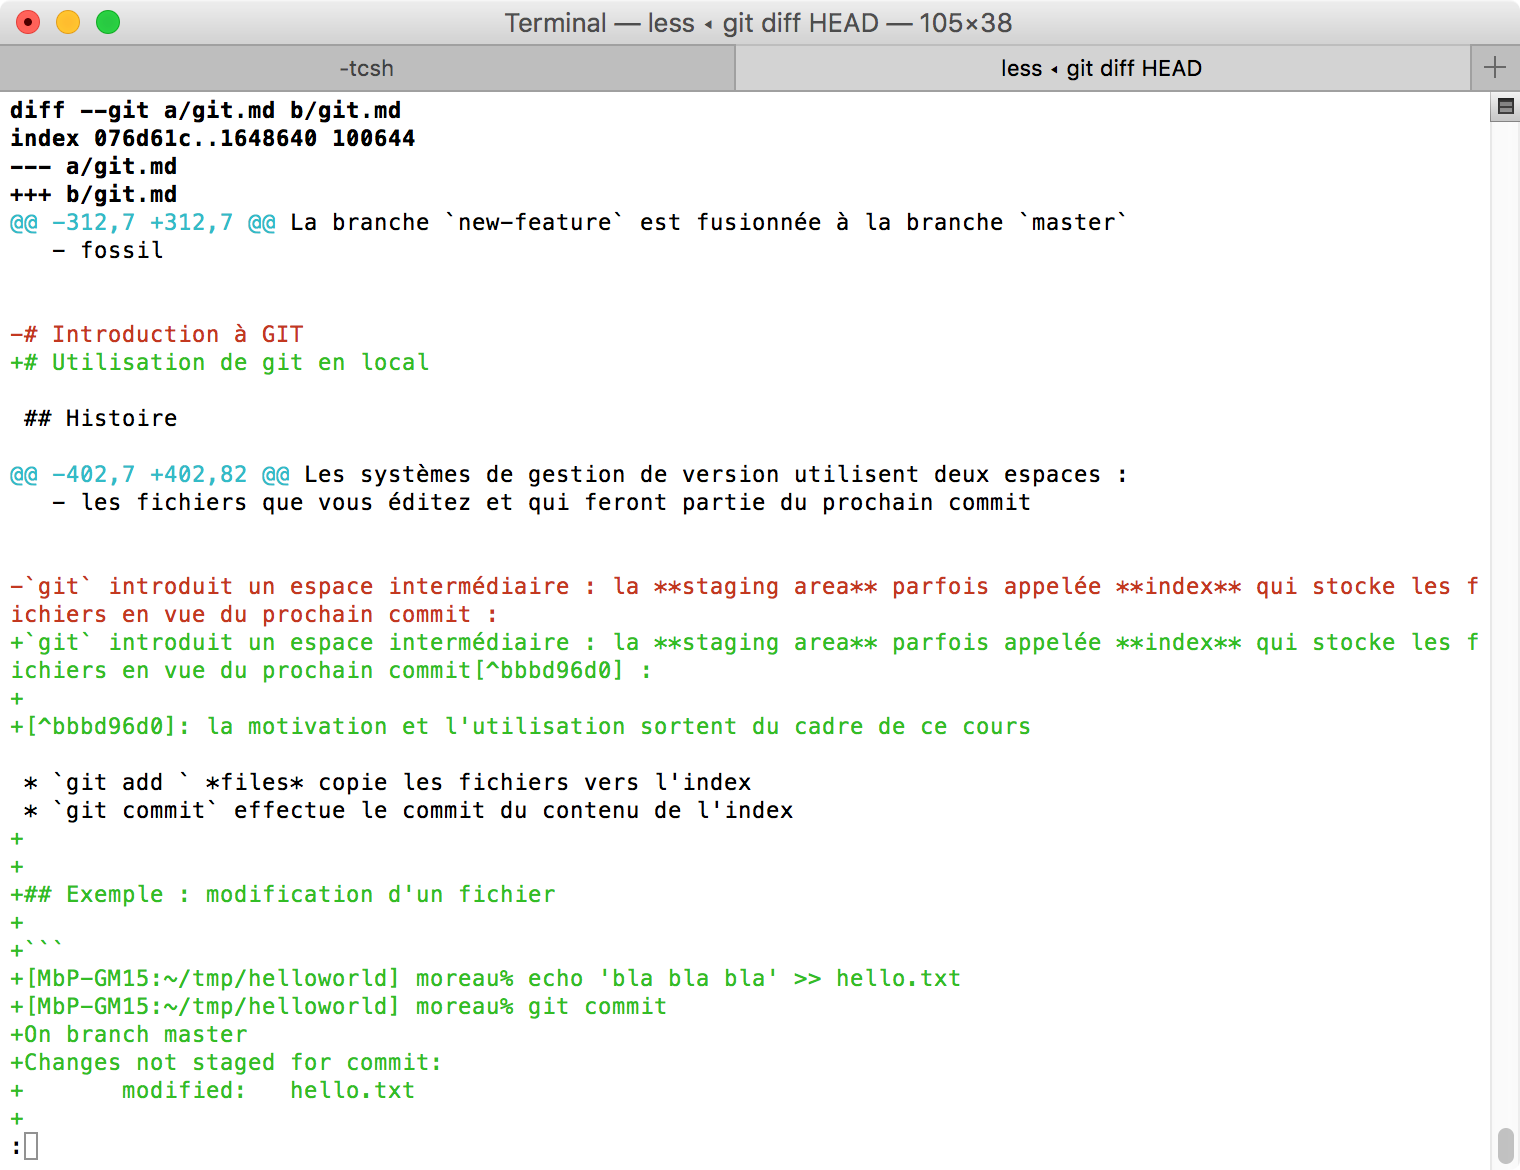
\includegraphics[width=0.5\textwidth]{images/cmd-diff.png}
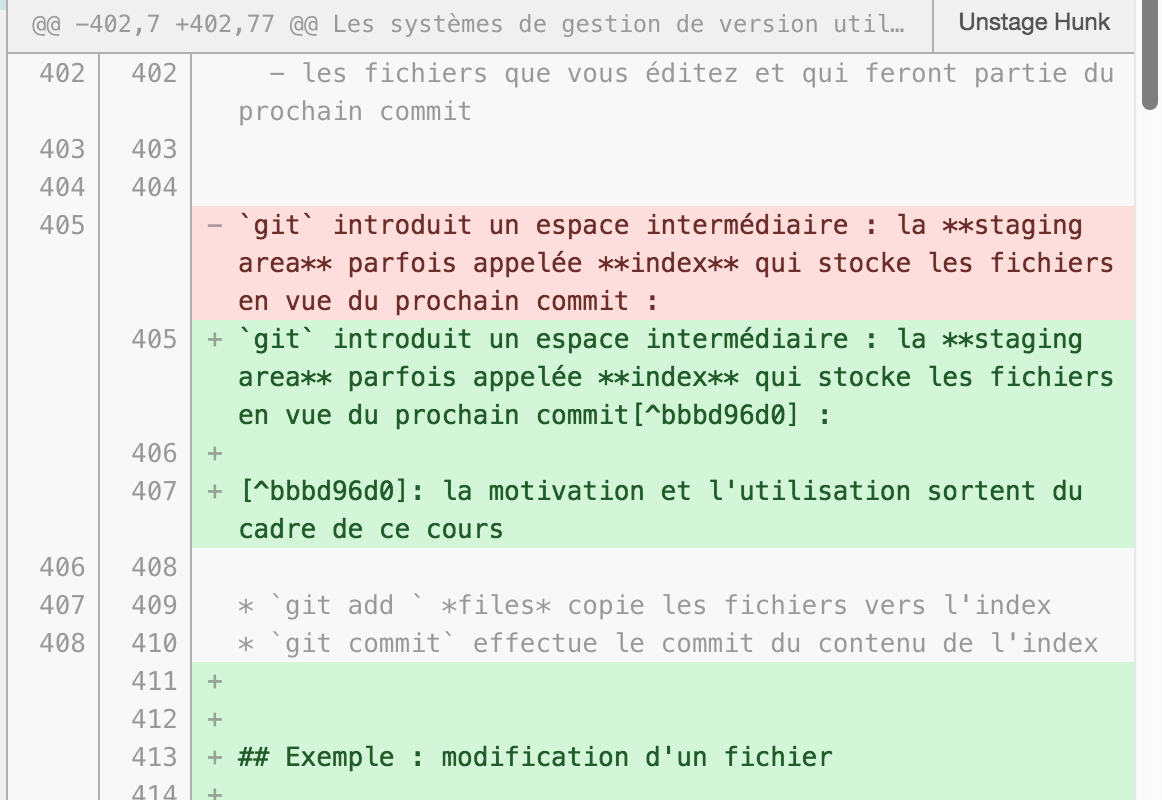
\includegraphics[width=0.5\textwidth]{images/atom-diff.png}

On verra que les outils sont encore plus perfectionnés pour le
développement collaboratif

\end{frame}

\begin{frame}[fragile]{%
\protect\hypertarget{revenir-en-arriuxe8re}{%
Revenir en arrière}}

\begin{itemize}
\tightlist
\item
  \texttt{git\ reset} annule les changements dans l’index
\item
  \texttt{git\ reset\ -\/-hard} annule les changements dans l’index
  \textbf{et} dans la copie de travail
\item
  \texttt{git\ checkout\ -\/-}\emph{path} restaure un fichier ou un
  répertoire tel qu’il apparait dans l’index (revient de la copie de
  travail à l’état au dernier \texttt{git\ add})
\end{itemize}

\end{frame}

\begin{frame}[fragile]{%
\protect\hypertarget{autres-commandes-locales}{%
Autres commandes locales}}

\begin{itemize}
\tightlist
\item
  \texttt{git\ status} : donne l’état de l’index et de la copie de
  travail (la liste des modifications prises en compte ou non)
\item
  \texttt{git\ show} : donne les détail d’un commit
\item
  \texttt{git\ log} : donne l’historique
\item
  \texttt{git\ mv} : déplace ou renomme un fichier/répertoire
\item
  \texttt{git\ tag} : création et suppression des tags
\end{itemize}

\end{frame}

\hypertarget{branches-et-fusion}{%
\section{Branches et fusion}\label{branches-et-fusion}}

\begin{frame}{%
\protect\hypertarget{comment-git-guxe8re-t-il-son-historique}{%
Comment git gère-t-il son historique ?}}

\begin{columns}[T]
\begin{column}{0.40\textwidth}
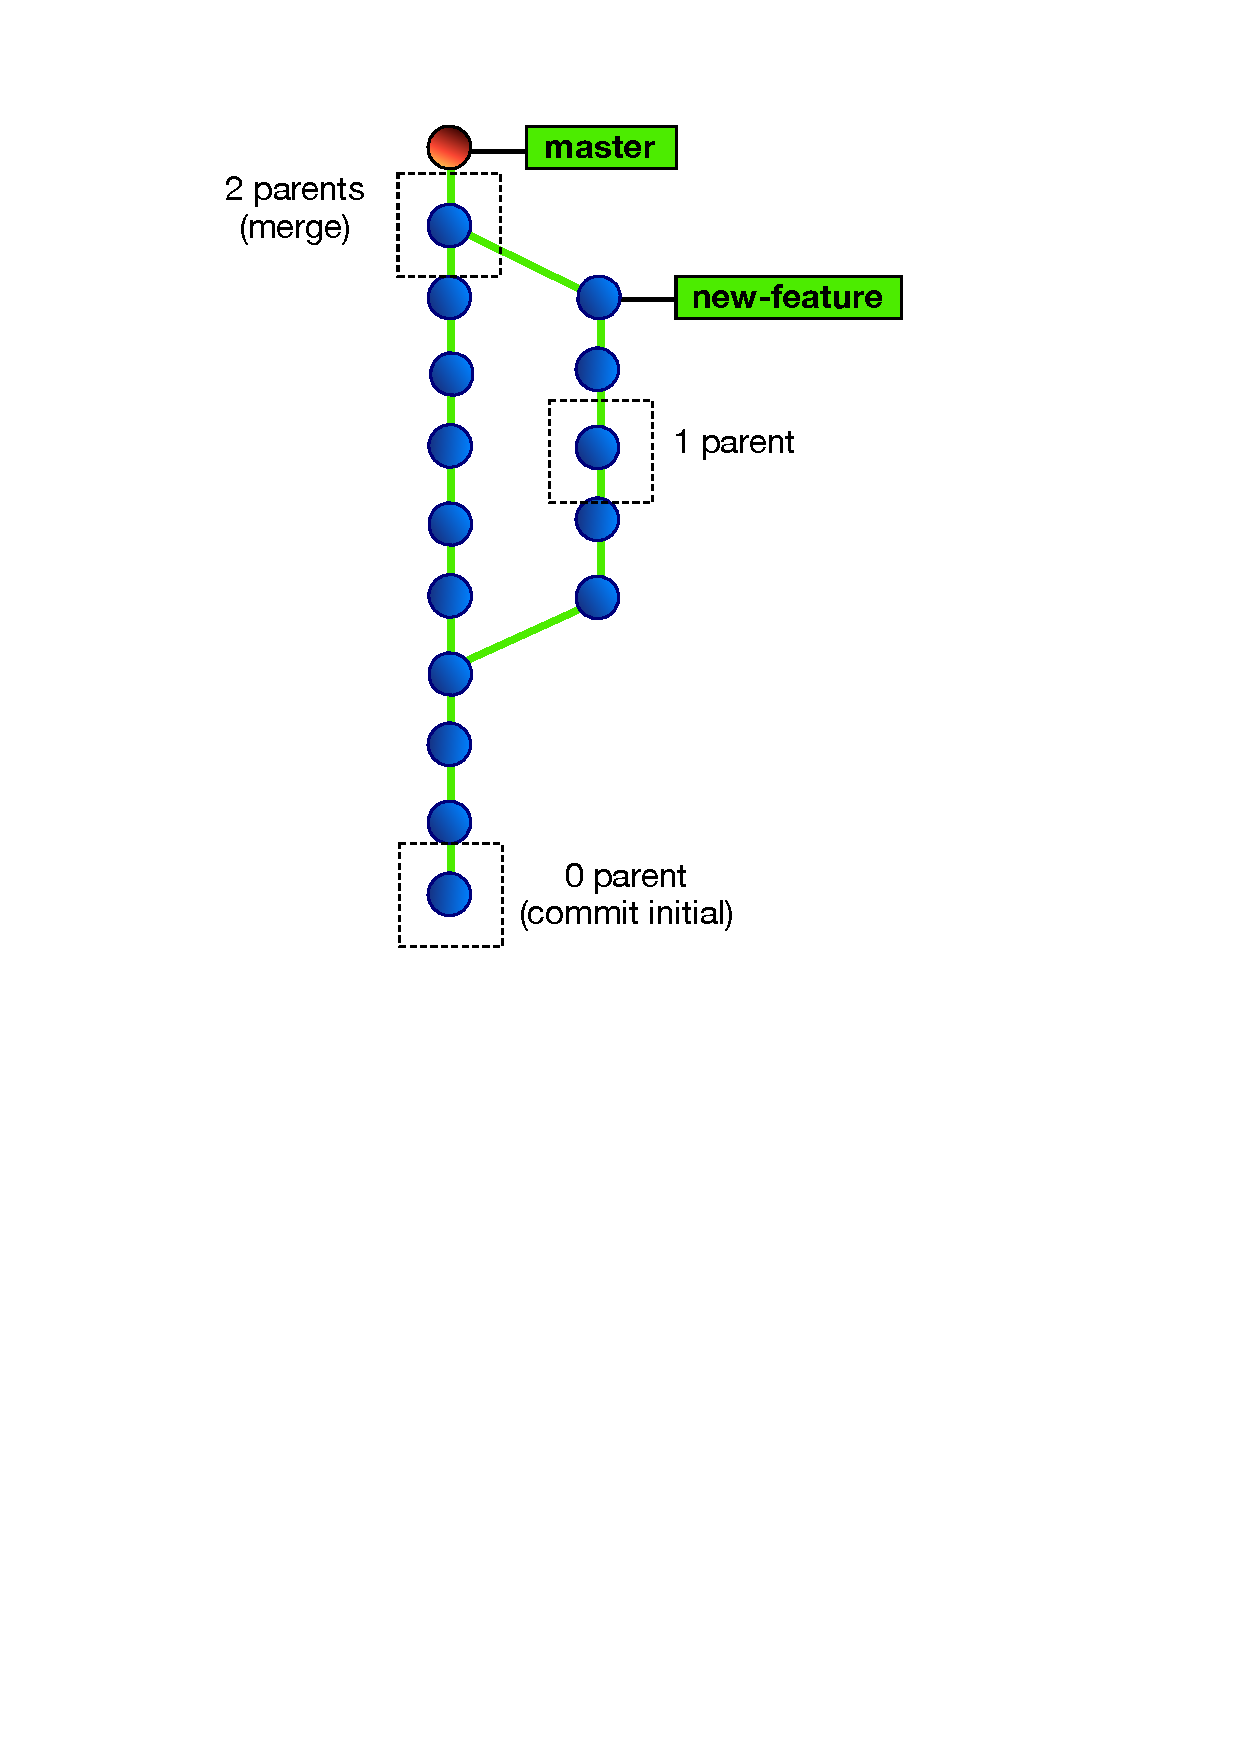
\includegraphics[width=1\textwidth]{images/dag.pdf}
\end{column}

\begin{column}{0.60\textwidth}
Chaque objet de \textbf{commit} possède sa propre liste de
\textbf{commit} parents :

\begin{itemize}
\tightlist
\item
  0 parent : commit initial
\item
  1 parent : commit ordinaire
\item
  2+ parents : résultat d’une fusion (merge) de branches
\end{itemize}

d’où cette notion de \emph{graphe acyclique orienté}.

en réalité, une branche est juste un pointeur sur le dernier commit.
\end{column}
\end{columns}

\end{frame}

\begin{frame}[fragile]{%
\protect\hypertarget{cruxe9ation-dune-nouvelle-branche}{%
Création d’une nouvelle branche}}

\begin{verbatim}
git checkout -b nouvelle_branche  [ depart ]
\end{verbatim}

\begin{itemize}
\tightlist
\item
  \emph{nouvelle\_branche} est le nom de la nouvelle branche
\item
  \emph{depart} est le point de départ (commit id, tag\ldots{}). Par
  défaut \texttt{git}utilise l’emplacement courant
\end{itemize}

\begin{verbatim}
[MbP-GM15:~/tmp/helloworld] moreau% git status
On branch master
nothing to commit, working tree clean
[MbP-GM15:~/tmp/helloworld] moreau% git checkout -b develop
Switched to a new branch 'develop'
[MbP-GM15:~/tmp/helloworld] moreau% git status
On branch develop
nothing to commit, working tree clean
\end{verbatim}

\end{frame}

\begin{frame}[fragile]{%
\protect\hypertarget{passer-dune-branche-uxe0-lautres}{%
Passer d’une branche à l’autres}}

\texttt{git\ checkout\ {[}-m{]}} \emph{branch\_name}

\begin{verbatim}
[MbP-GM15:~/tmp/helloworld] moreau% git status
On branch develop
nothing to commit, working tree clean
[MbP-GM15:~/tmp/helloworld] moreau% git checkout master
Switched to branch 'master'
\end{verbatim}

La commande ne fonctionne que si le copie de travail est propre.
L’option \texttt{-m} permet de demander une fusion vers la branche de
destination.

\end{frame}

\begin{frame}[fragile]{%
\protect\hypertarget{fusion-de-branches}{%
Fusion de branches}}

\texttt{git\ merge} \emph{other\_branch}

fusionne les changements effectués dans \emph{other\_branch} vers la
branche courante.

\textbf{Attention} : cette commande n’est pas symétrique !

\begin{verbatim}
[MbP-GM15:~/tmp/helloworld] moreau% git add toto.txt
[MbP-GM15:~/tmp/helloworld] moreau% git commit
[develop 9d7c832] test
 1 file changed, 1 insertion(+)
 create mode 100644 toto.txt
[MbP-GM15:~/tmp/helloworld] moreau% git checkout master
Switched to branch 'master'
[MbP-GM15:~/tmp/helloworld] moreau% git merge develop
Updating 388f711..9d7c832
Fast-forward
 toto.txt | 1 +
 1 file changed, 1 insertion(+)
 create mode 100644 toto.txt
\end{verbatim}

\end{frame}

\begin{frame}[fragile]{%
\protect\hypertarget{quelques-remarques-sur-la-fusion}{%
Quelques remarques sur la fusion}}

\begin{itemize}
\tightlist
\item
  Le résultat d’un \texttt{git\ merge} fait immédiatement l’objet d’un
  commit (sauf en cas de conflit)
\item
  Le nouvel objet de commit a \textbf{deux parents}

  \begin{itemize}
  \tightlist
  \item
    l’historique de la fusion est donc enregistré
  \end{itemize}
\item
  \texttt{git\ merge} s’applique uniquement aux changements effectués
  dans l’autre branche depuis le dernier ancêtre commun

  \begin{itemize}
  \tightlist
  \item
    s’il y a déjà eu un \texttt{merge}, seuls les changements depuis le
    dernier \texttt{merge} seront pris en compte
  \end{itemize}
\end{itemize}

\end{frame}

\begin{frame}{%
\protect\hypertarget{exemple-112}{%
Exemple (1/12)}}

\begin{columns}[T]
\begin{column}{0.40\textwidth}
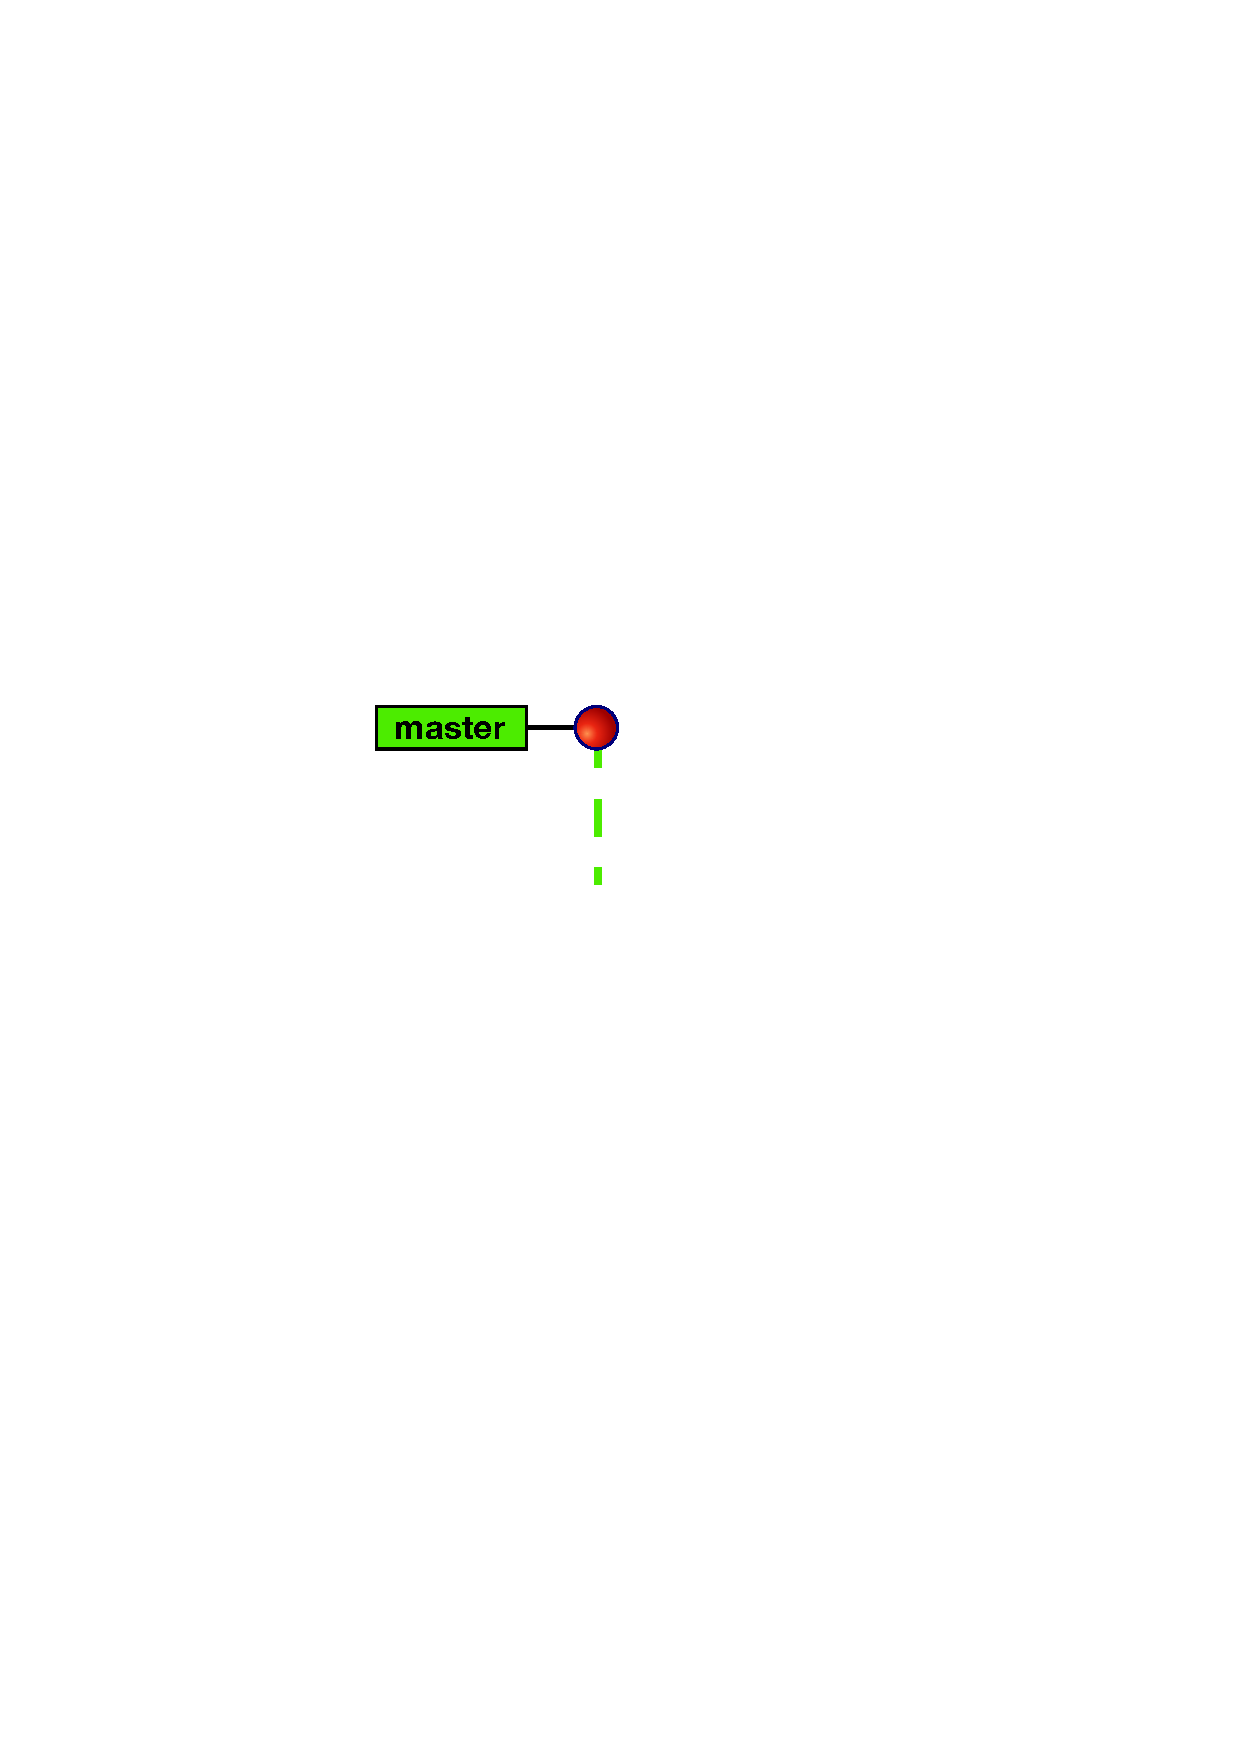
\includegraphics[width=1\textwidth]{images/branch1.pdf}
\end{column}

\begin{column}{0.60\textwidth}
Situation initiale
\end{column}
\end{columns}

\end{frame}

\begin{frame}[fragile]{%
\protect\hypertarget{exemple-212}{%
Exemple (2/12)}}

\begin{columns}[T]
\begin{column}{0.40\textwidth}
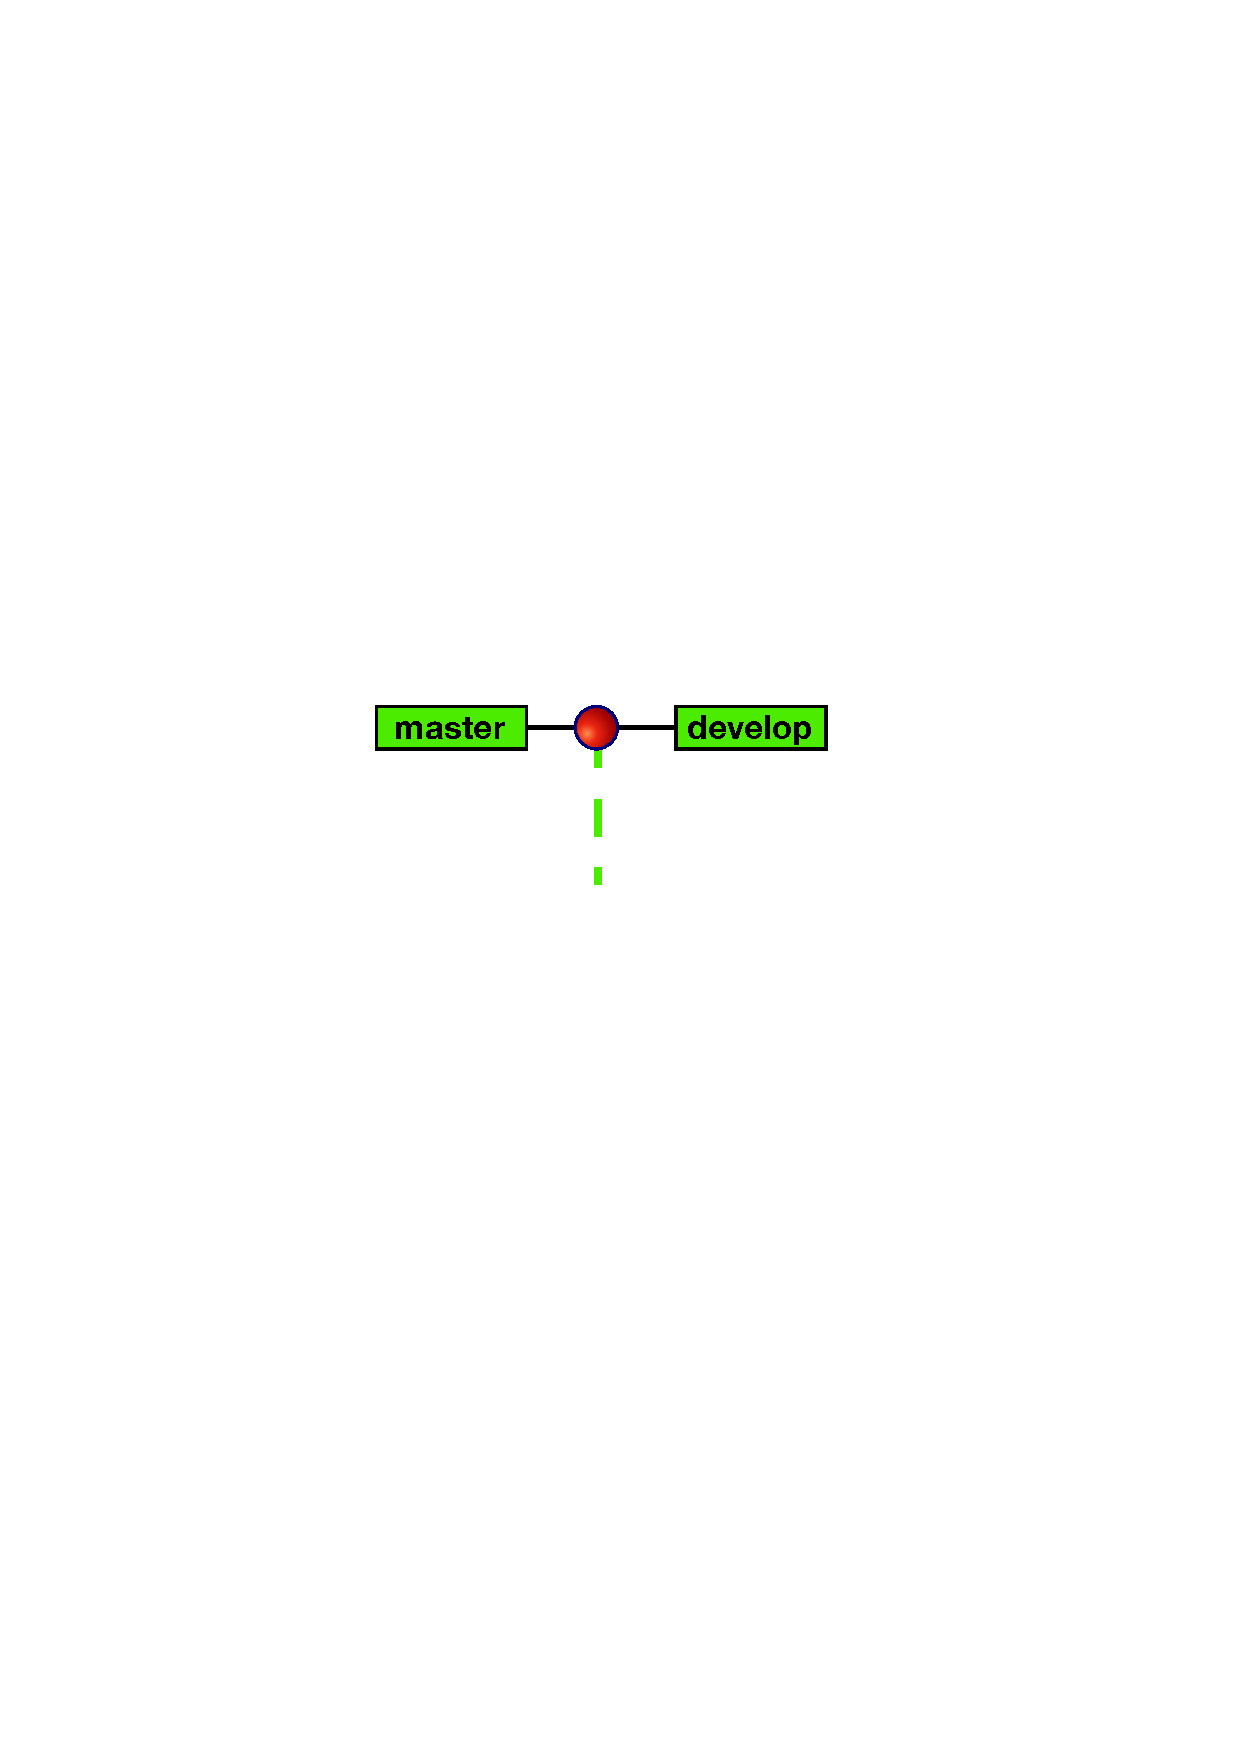
\includegraphics[width=1\textwidth]{images/branch2.pdf}
\end{column}

\begin{column}{0.60\textwidth}
\texttt{git\ checkout\ -b\ develop}
\end{column}
\end{columns}

\end{frame}

\begin{frame}[fragile]{%
\protect\hypertarget{exemple-312}{%
Exemple (3/12)}}

\begin{columns}[T]
\begin{column}{0.40\textwidth}
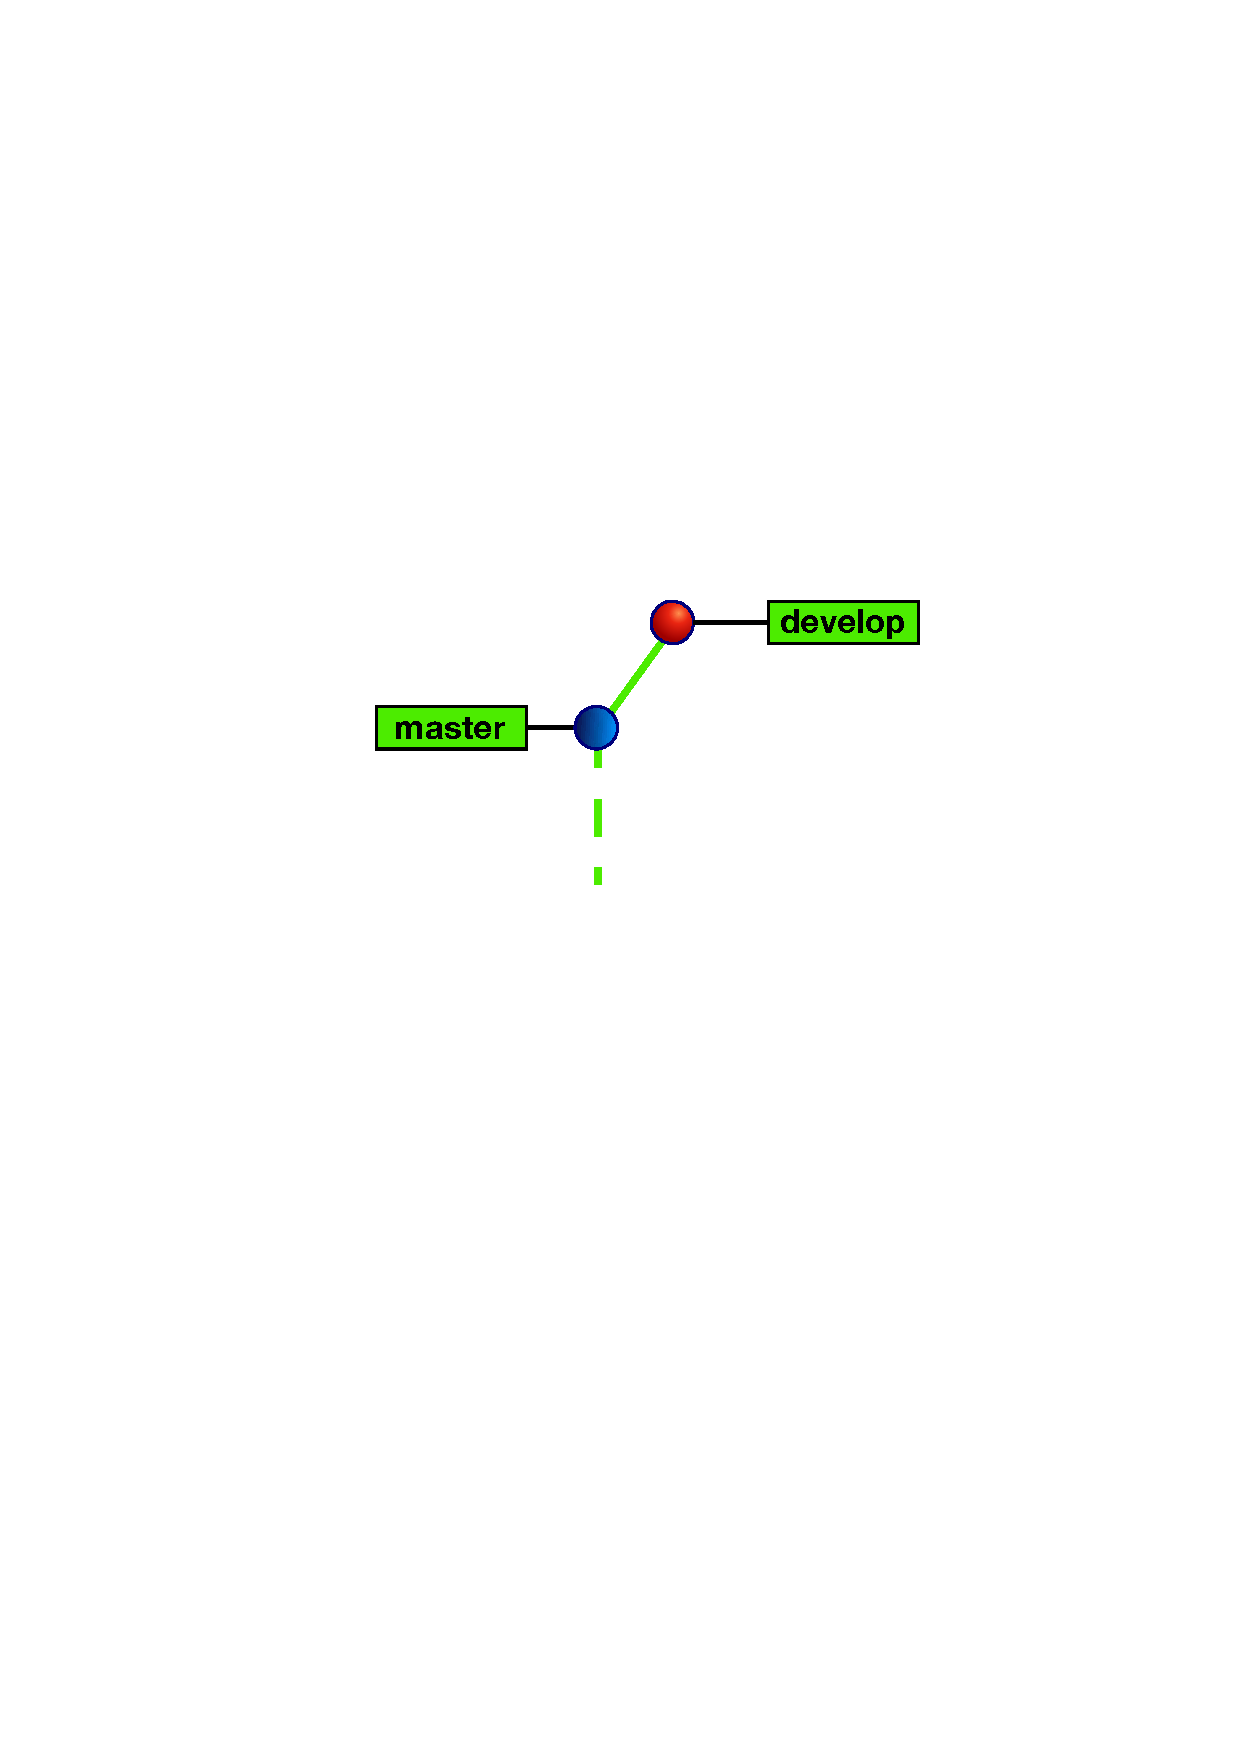
\includegraphics[width=1\textwidth]{images/branch3.pdf}
\end{column}

\begin{column}{0.60\textwidth}
\texttt{git\ commit}
\end{column}
\end{columns}

\end{frame}

\begin{frame}[fragile]{%
\protect\hypertarget{exemple-412}{%
Exemple (4/12)}}

\begin{columns}[T]
\begin{column}{0.40\textwidth}
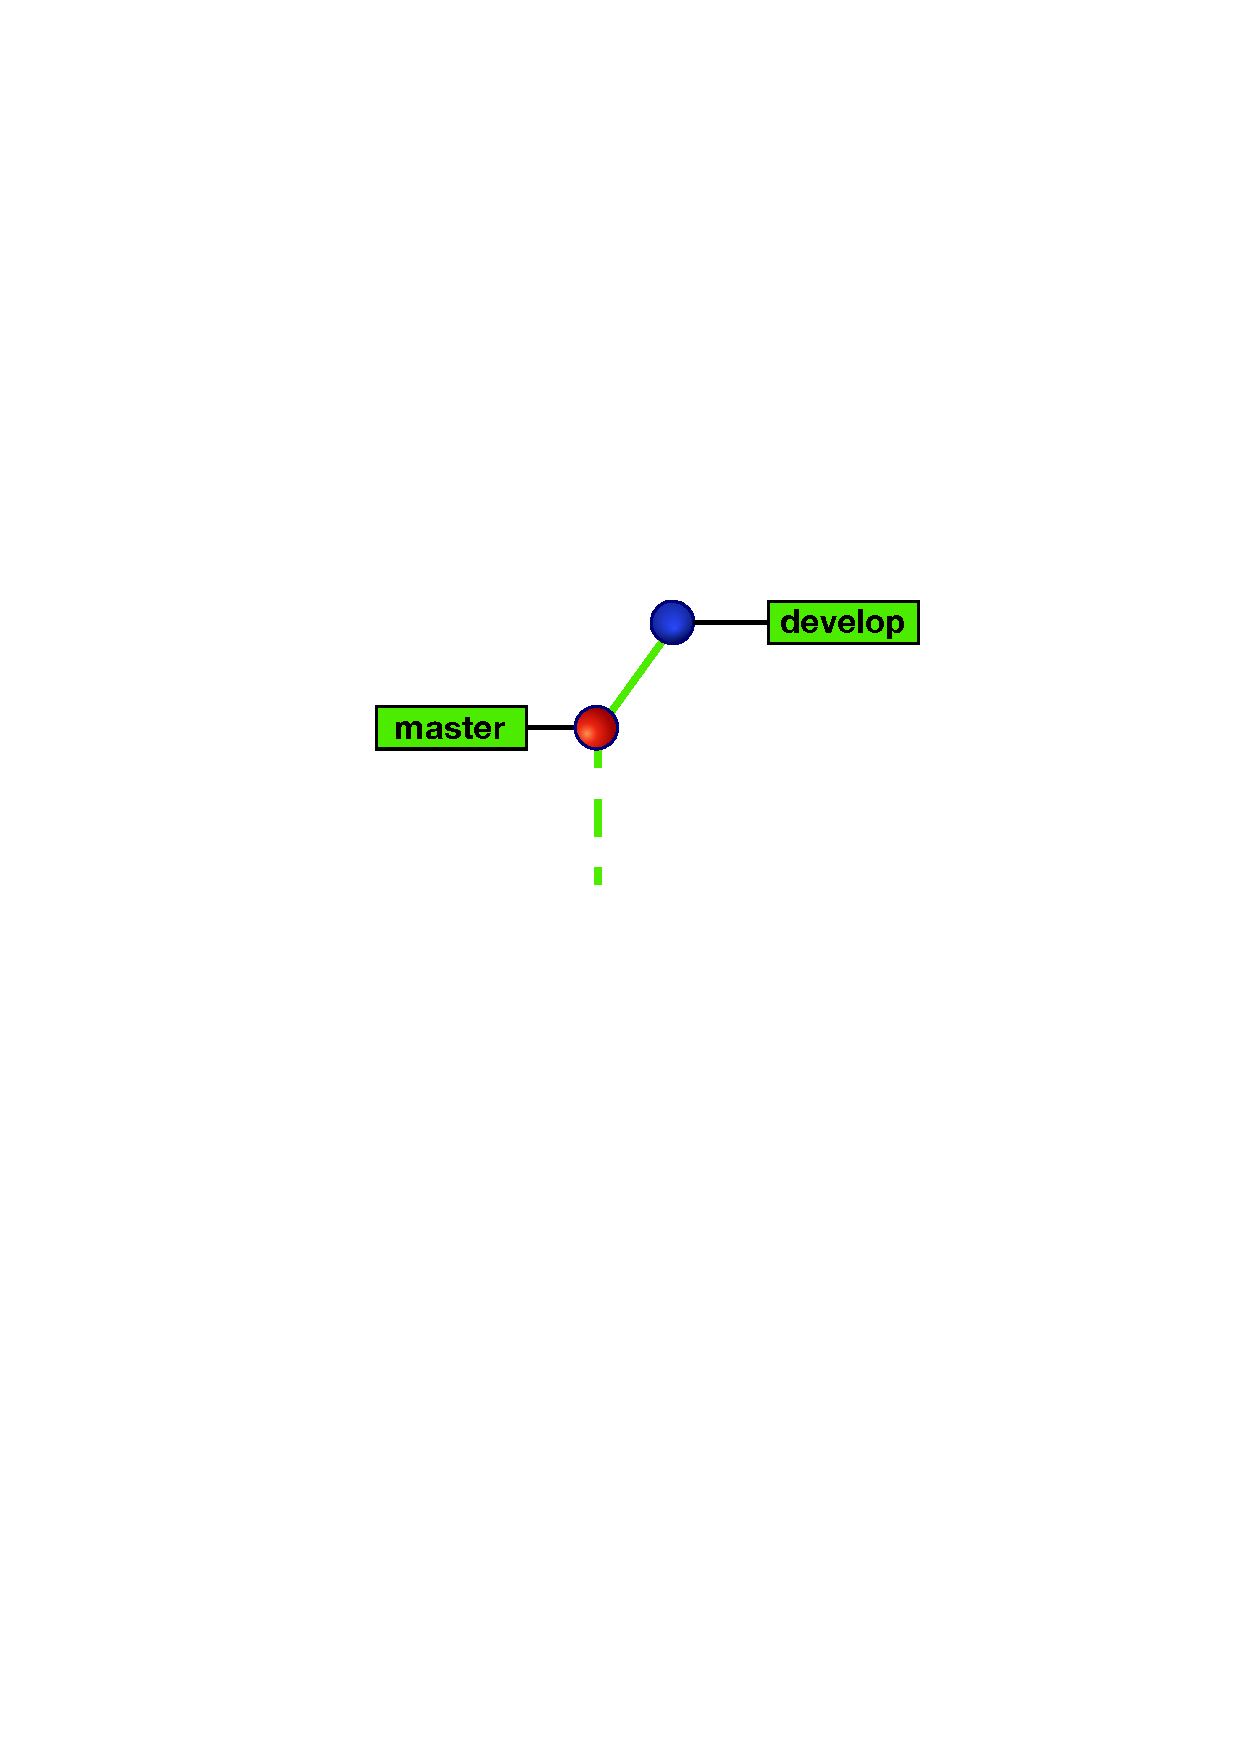
\includegraphics[width=1\textwidth]{images/branch4.pdf}
\end{column}

\begin{column}{0.60\textwidth}
\texttt{git\ checkout\ master}
\end{column}
\end{columns}

\end{frame}

\begin{frame}[fragile]{%
\protect\hypertarget{exemple-512}{%
Exemple (5/12)}}

\begin{columns}[T]
\begin{column}{0.40\textwidth}
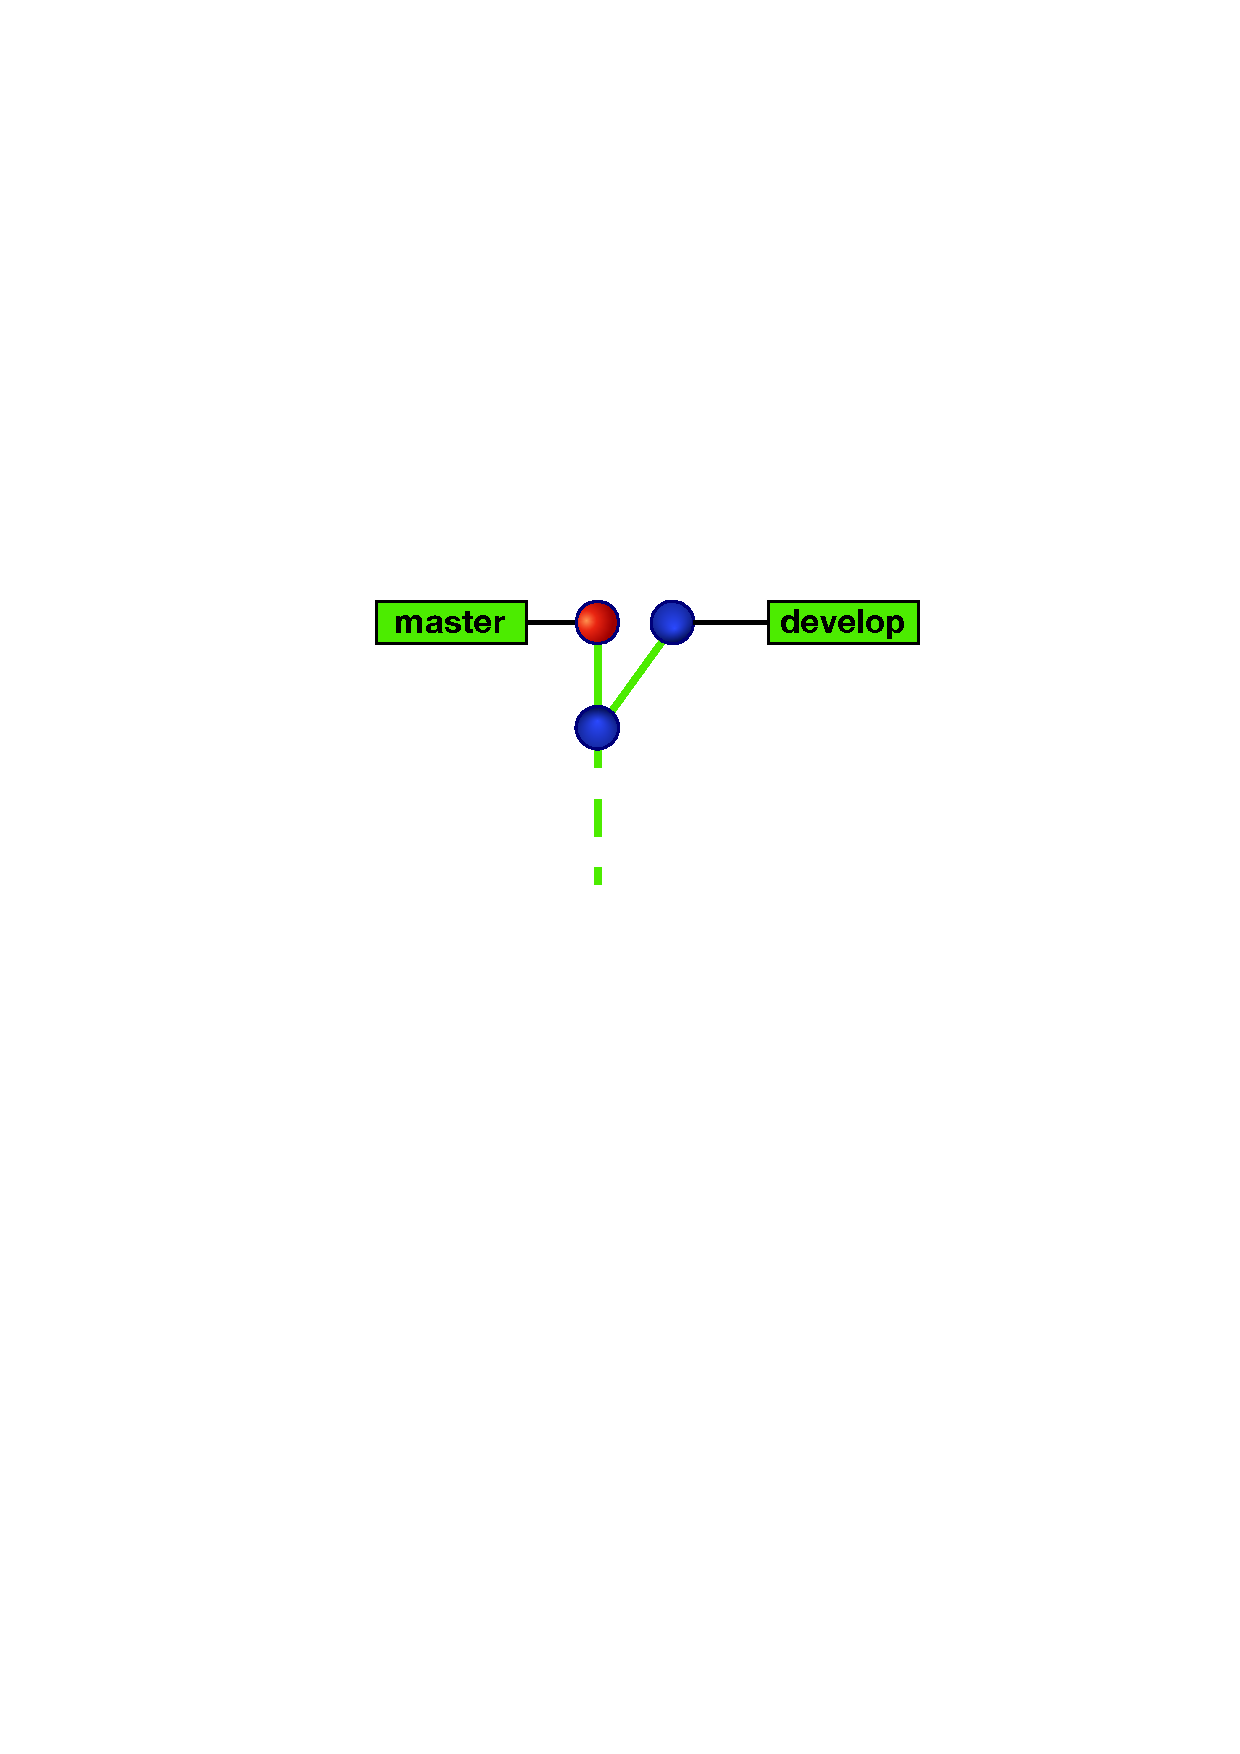
\includegraphics[width=1\textwidth]{images/branch5.pdf}
\end{column}

\begin{column}{0.60\textwidth}
\texttt{git\ commit}
\end{column}
\end{columns}

\end{frame}

\begin{frame}[fragile]{%
\protect\hypertarget{exemple-612}{%
Exemple (6/12)}}

\begin{columns}[T]
\begin{column}{0.40\textwidth}
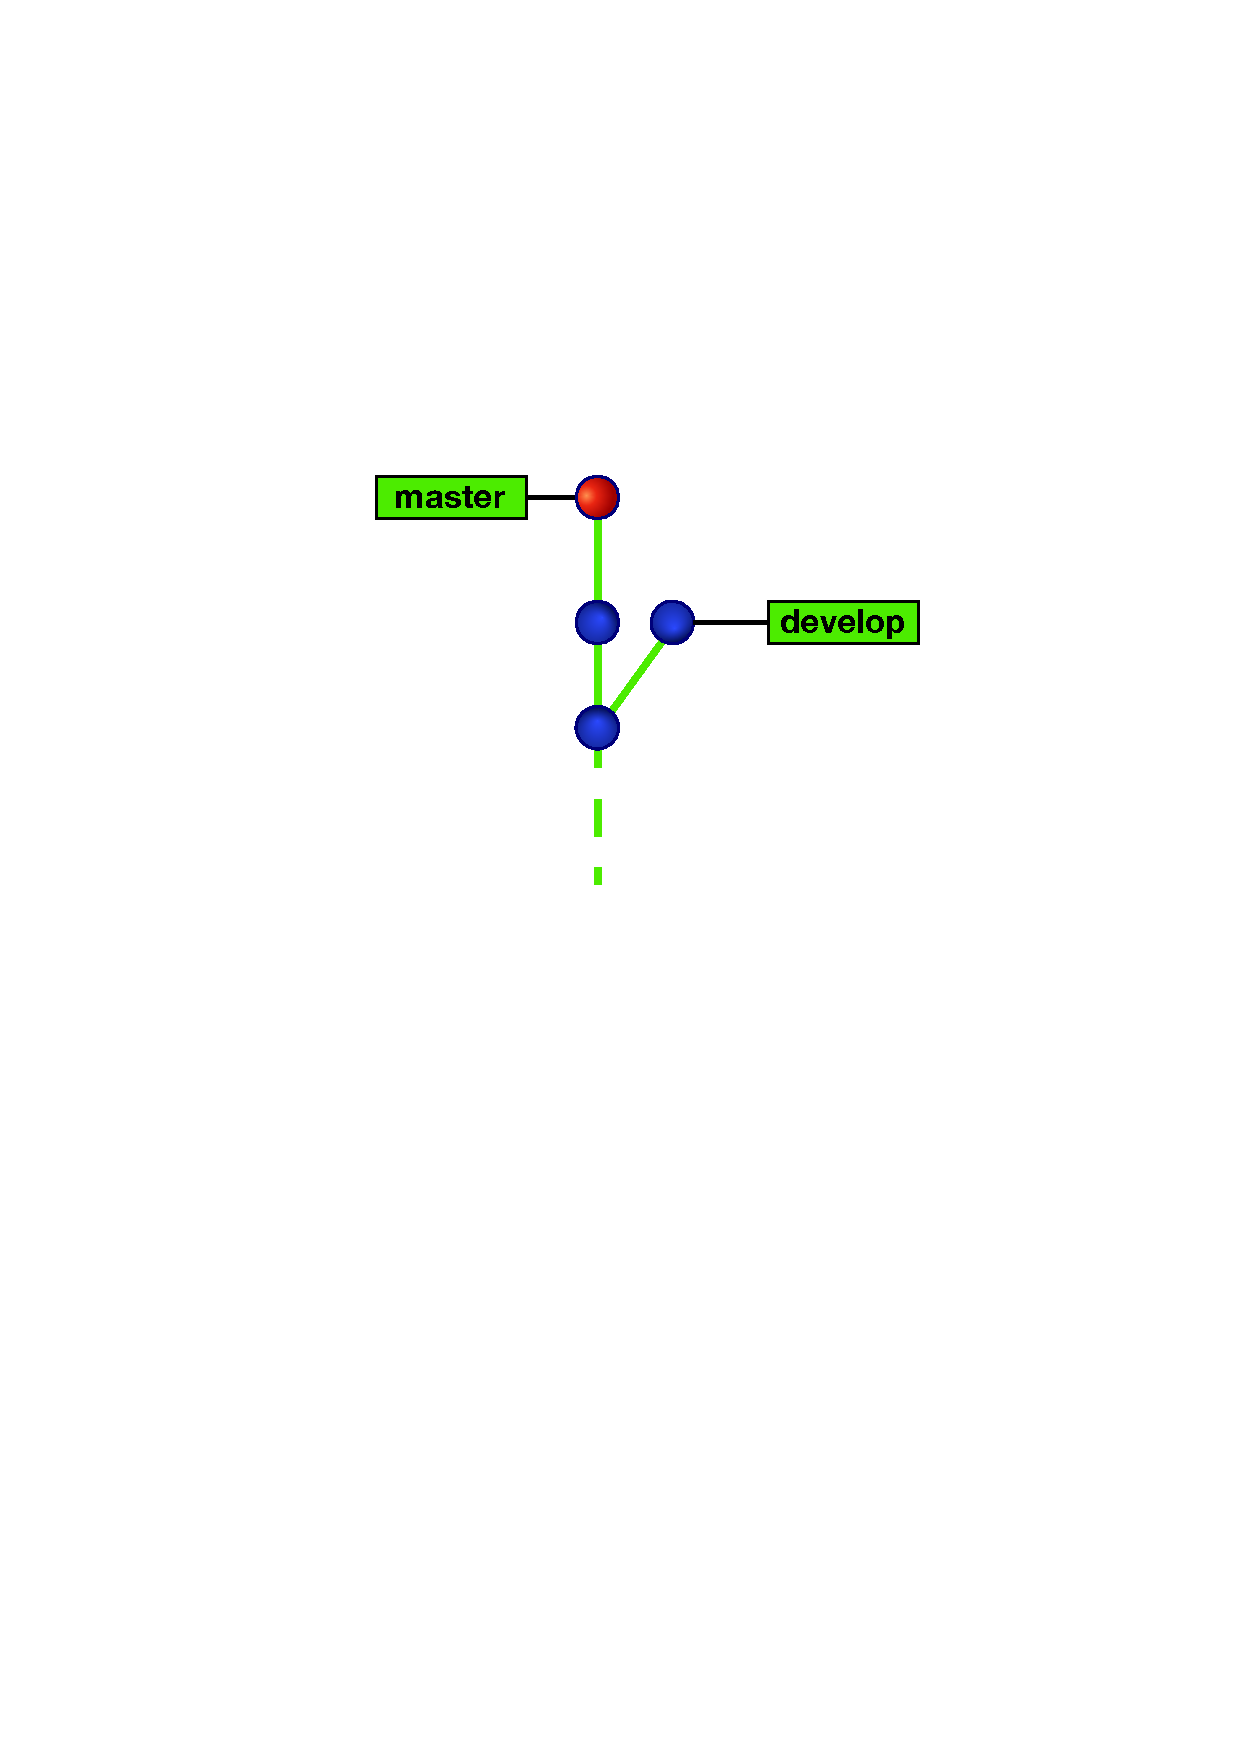
\includegraphics[width=1\textwidth]{images/branch6.pdf}
\end{column}

\begin{column}{0.60\textwidth}
\texttt{git\ commit}
\end{column}
\end{columns}

\end{frame}

\begin{frame}[fragile]{%
\protect\hypertarget{exemple-712}{%
Exemple (7/12)}}

\begin{columns}[T]
\begin{column}{0.40\textwidth}
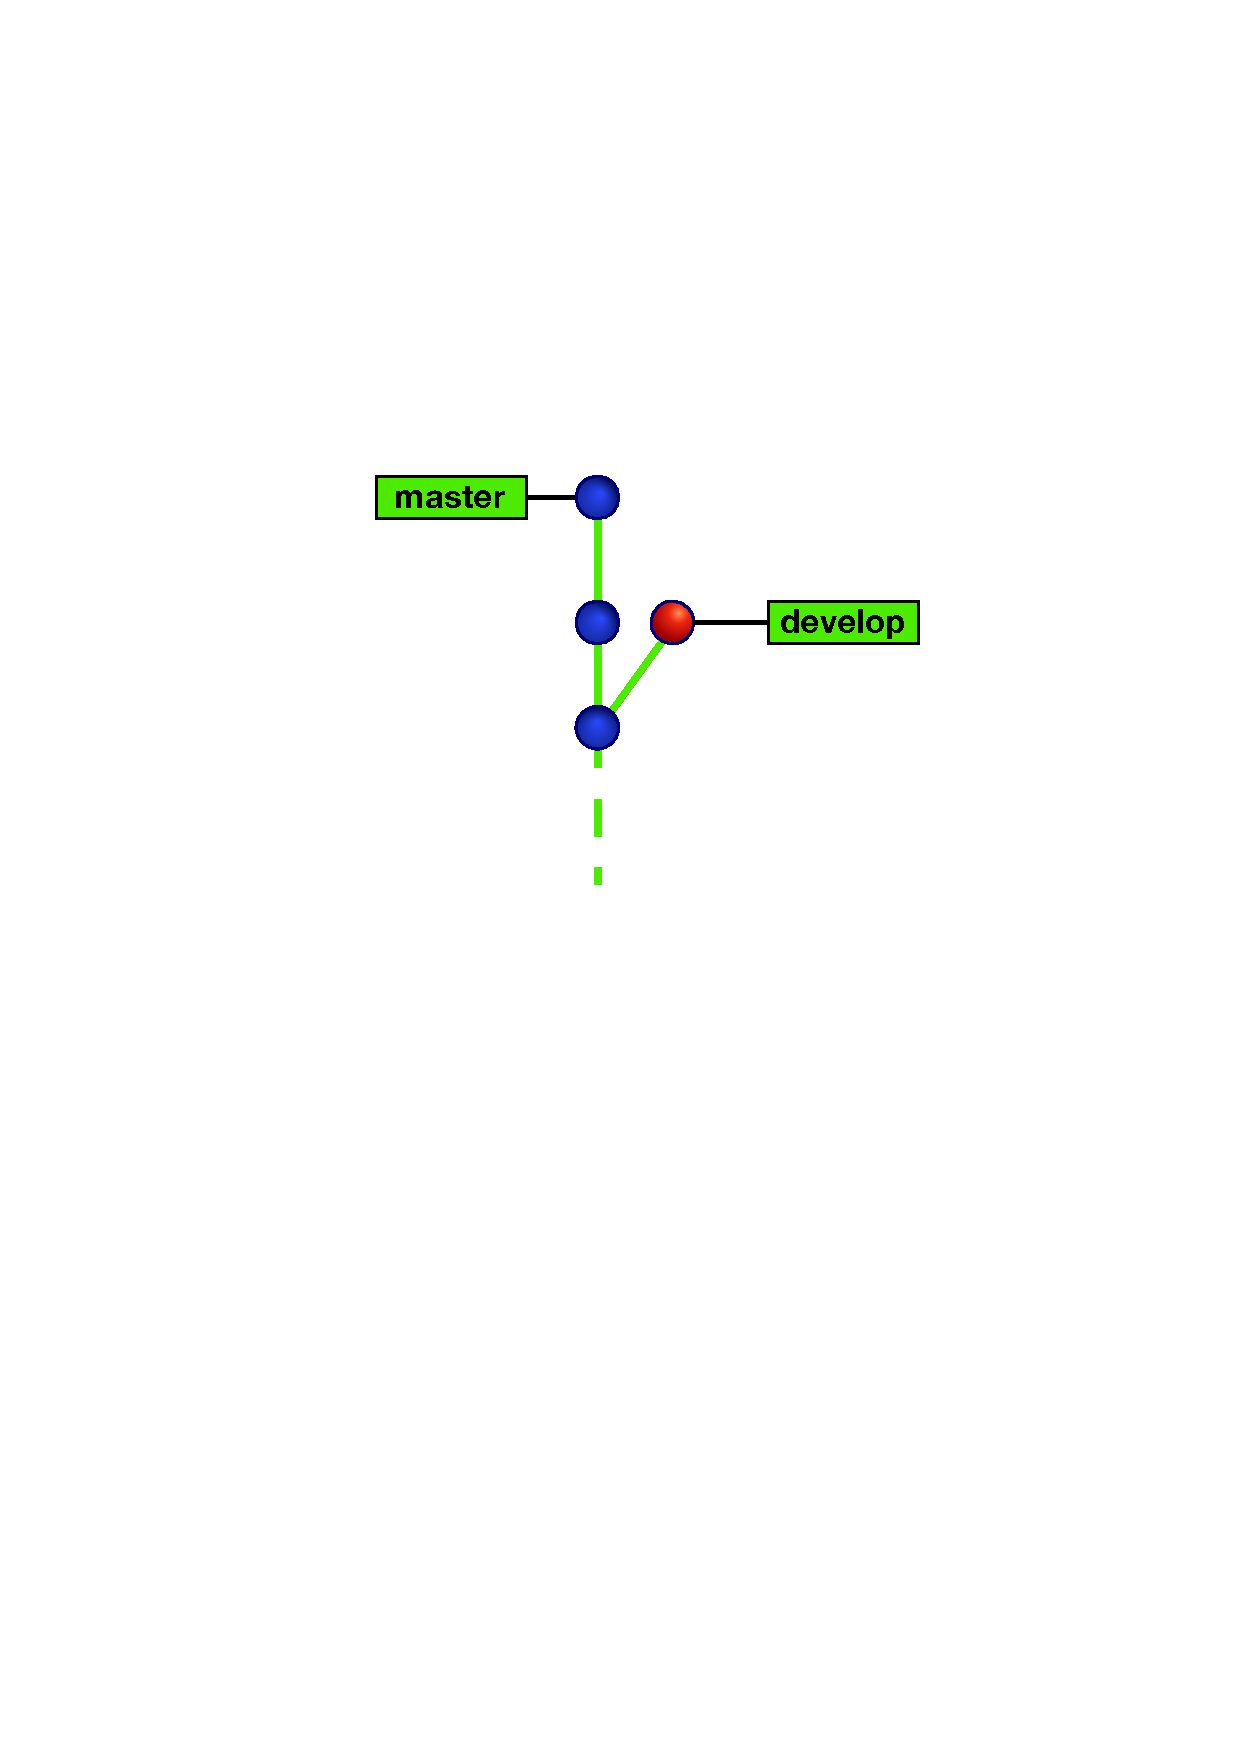
\includegraphics[width=1\textwidth]{images/branch7.pdf}
\end{column}

\begin{column}{0.60\textwidth}
\texttt{git\ checkout\ develop}
\end{column}
\end{columns}

\end{frame}

\begin{frame}[fragile]{%
\protect\hypertarget{exemple-812}{%
Exemple (8/12)}}

\begin{columns}[T]
\begin{column}{0.40\textwidth}
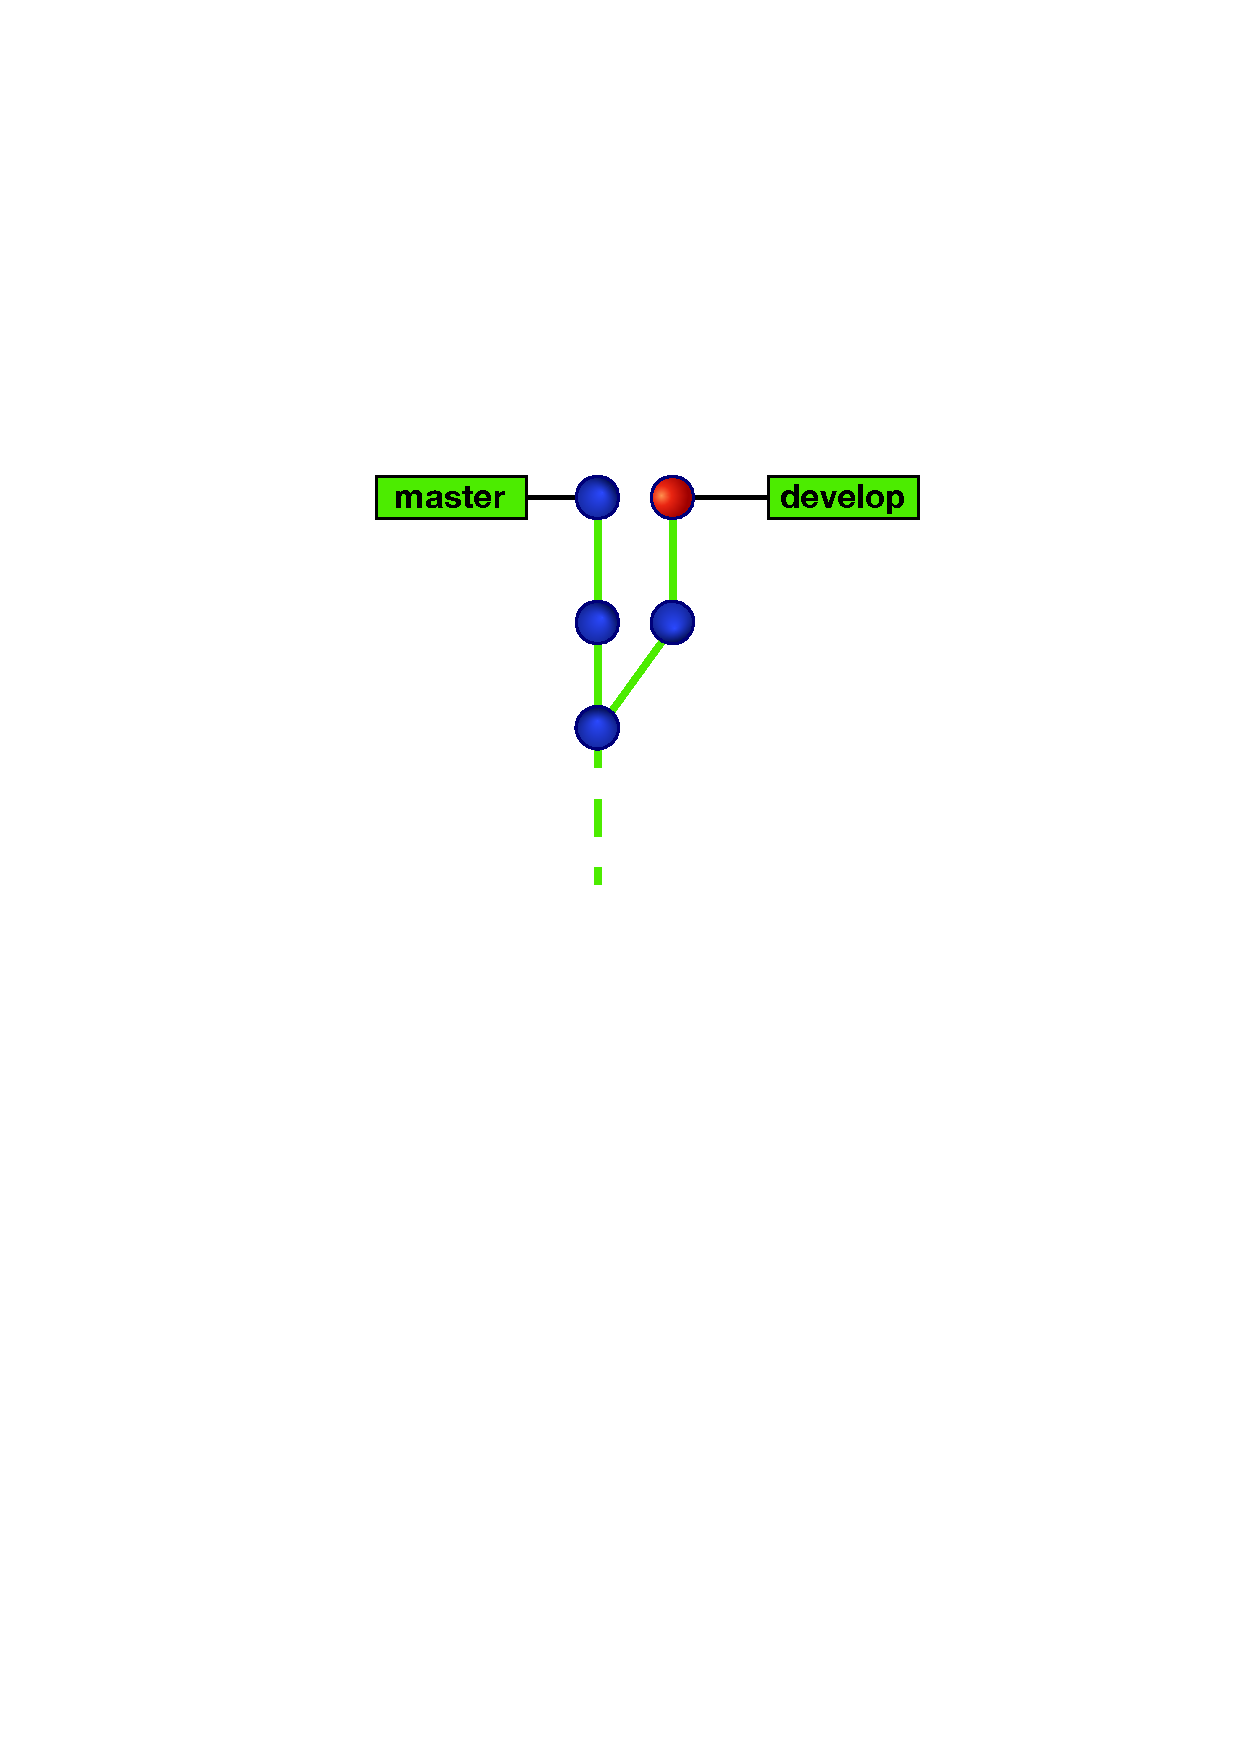
\includegraphics[width=1\textwidth]{images/branch8.pdf}
\end{column}

\begin{column}{0.60\textwidth}
\texttt{git\ commit}
\end{column}
\end{columns}

\end{frame}

\begin{frame}[fragile]{%
\protect\hypertarget{exemple-912}{%
Exemple (9/12)}}

\begin{columns}[T]
\begin{column}{0.40\textwidth}
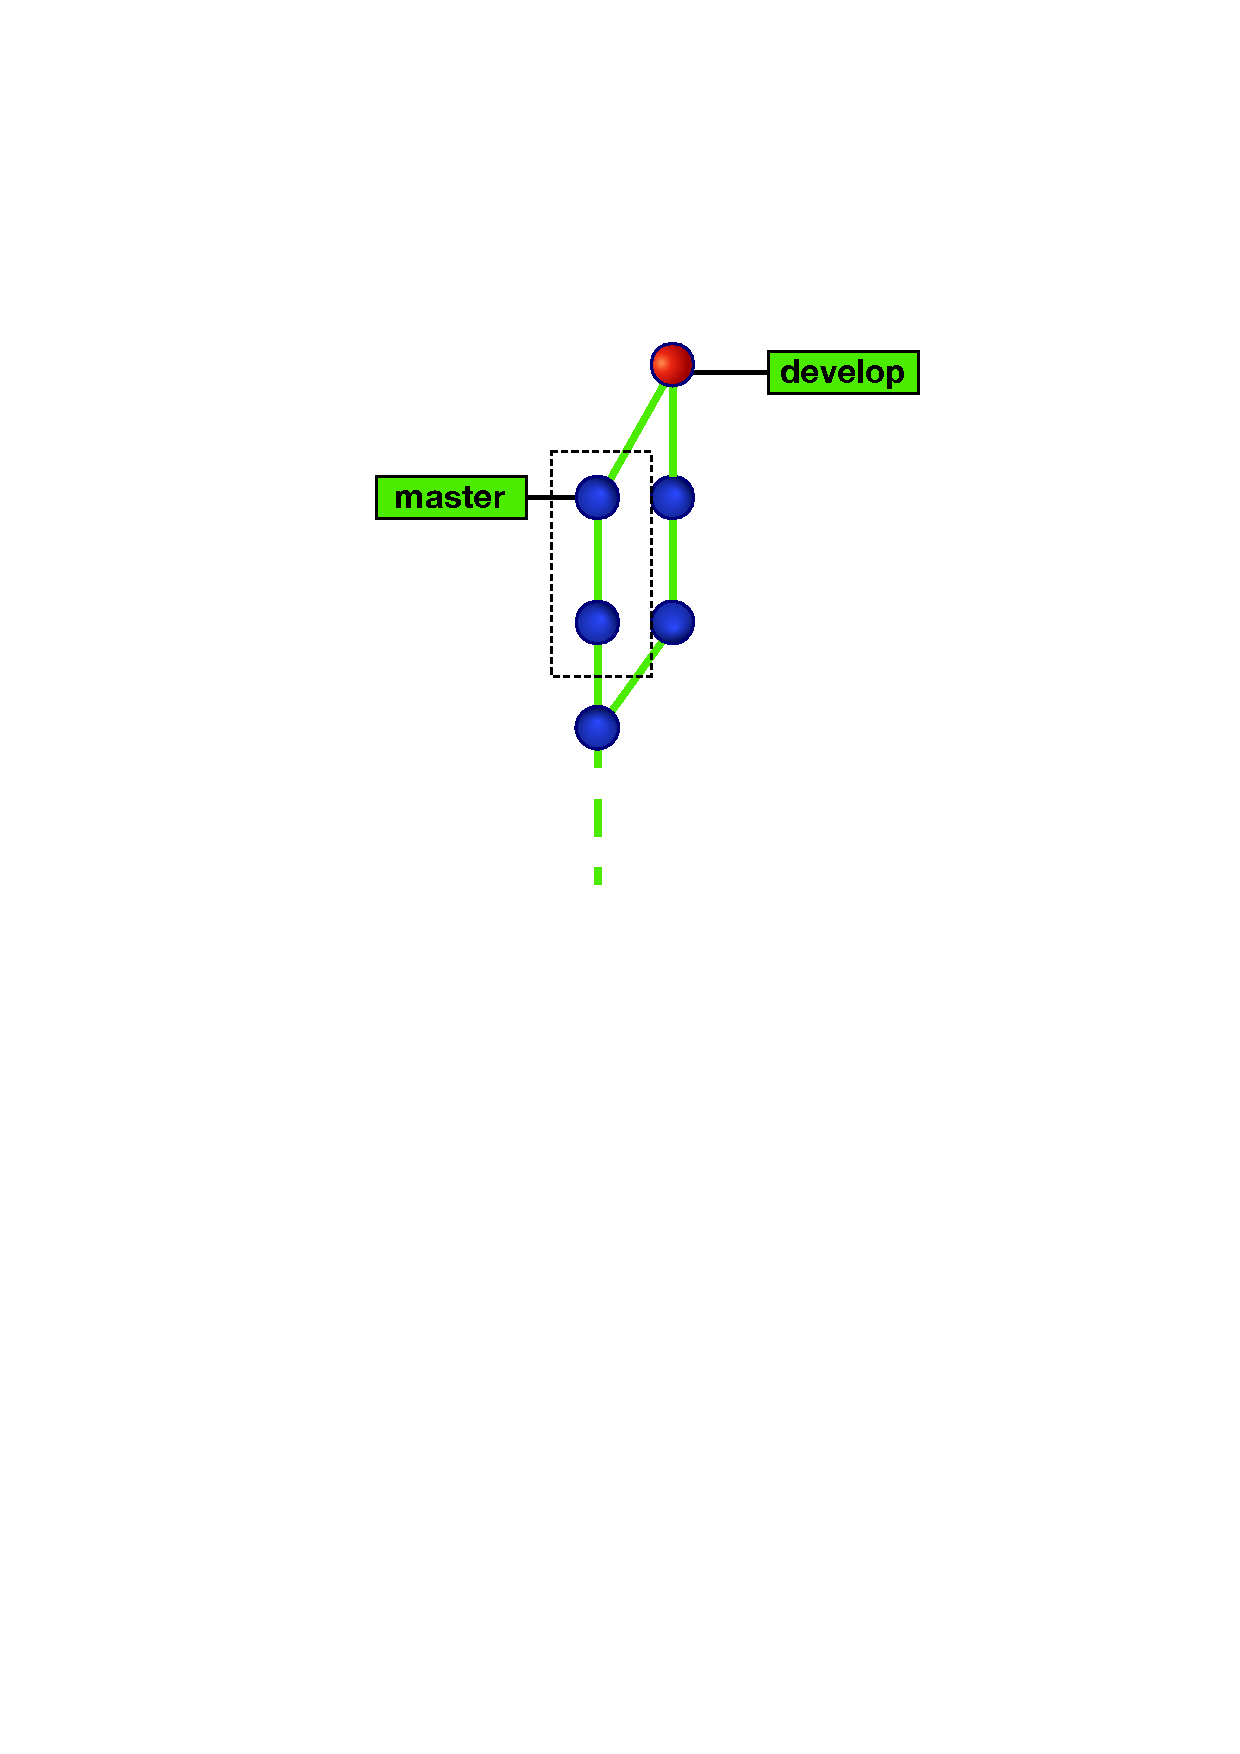
\includegraphics[width=1\textwidth]{images/branch9.pdf}
\end{column}

\begin{column}{0.60\textwidth}
\texttt{git\ merge\ master}

ici on demande bien la fusion de la branche \emph{master} vers la
branche \emph{develop}
\end{column}
\end{columns}

\end{frame}

\begin{frame}[fragile]{%
\protect\hypertarget{exemple-1012}{%
Exemple (10/12)}}

\begin{columns}[T]
\begin{column}{0.40\textwidth}
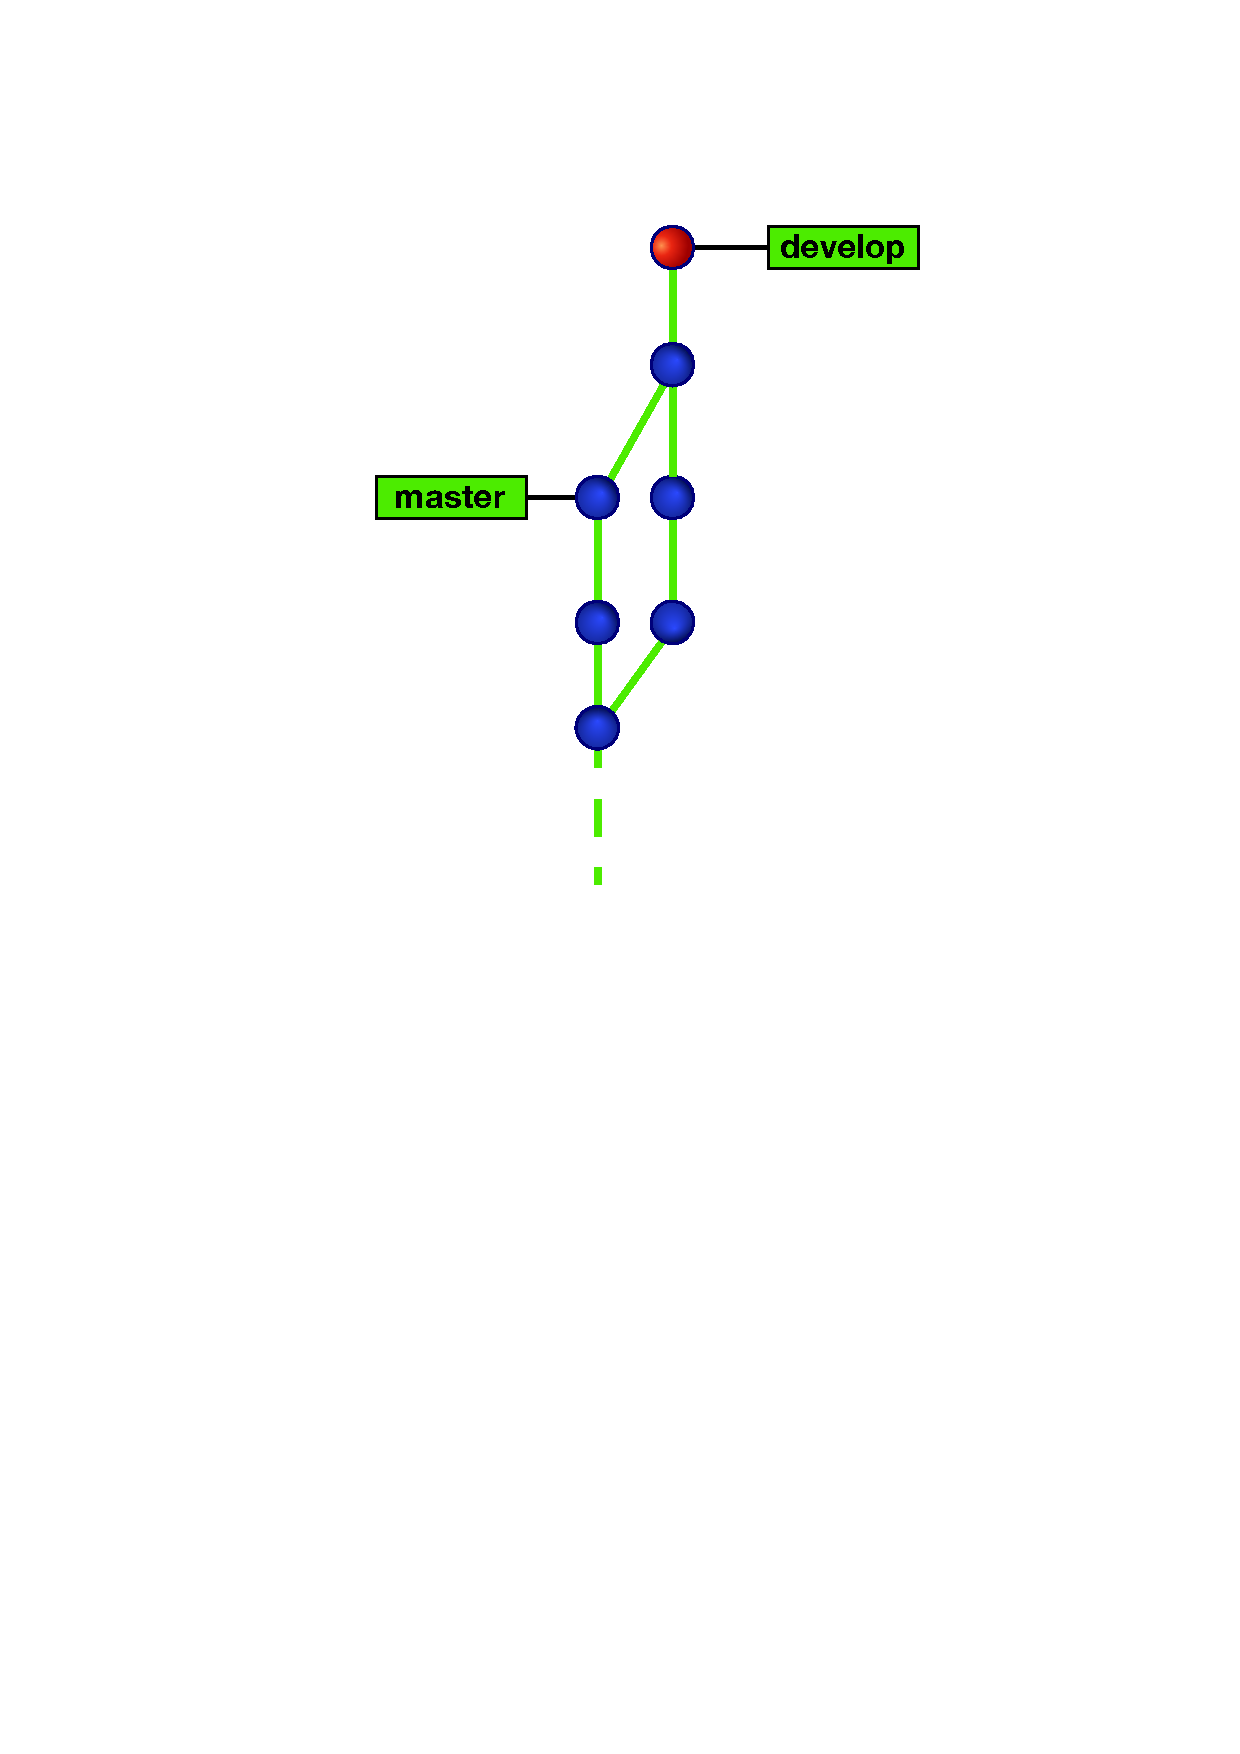
\includegraphics[width=1\textwidth]{images/branch10.pdf}
\end{column}

\begin{column}{0.60\textwidth}
\texttt{git\ commit}
\end{column}
\end{columns}

\end{frame}

\begin{frame}[fragile]{%
\protect\hypertarget{exemple-1112}{%
Exemple (11/12)}}

\begin{columns}[T]
\begin{column}{0.40\textwidth}
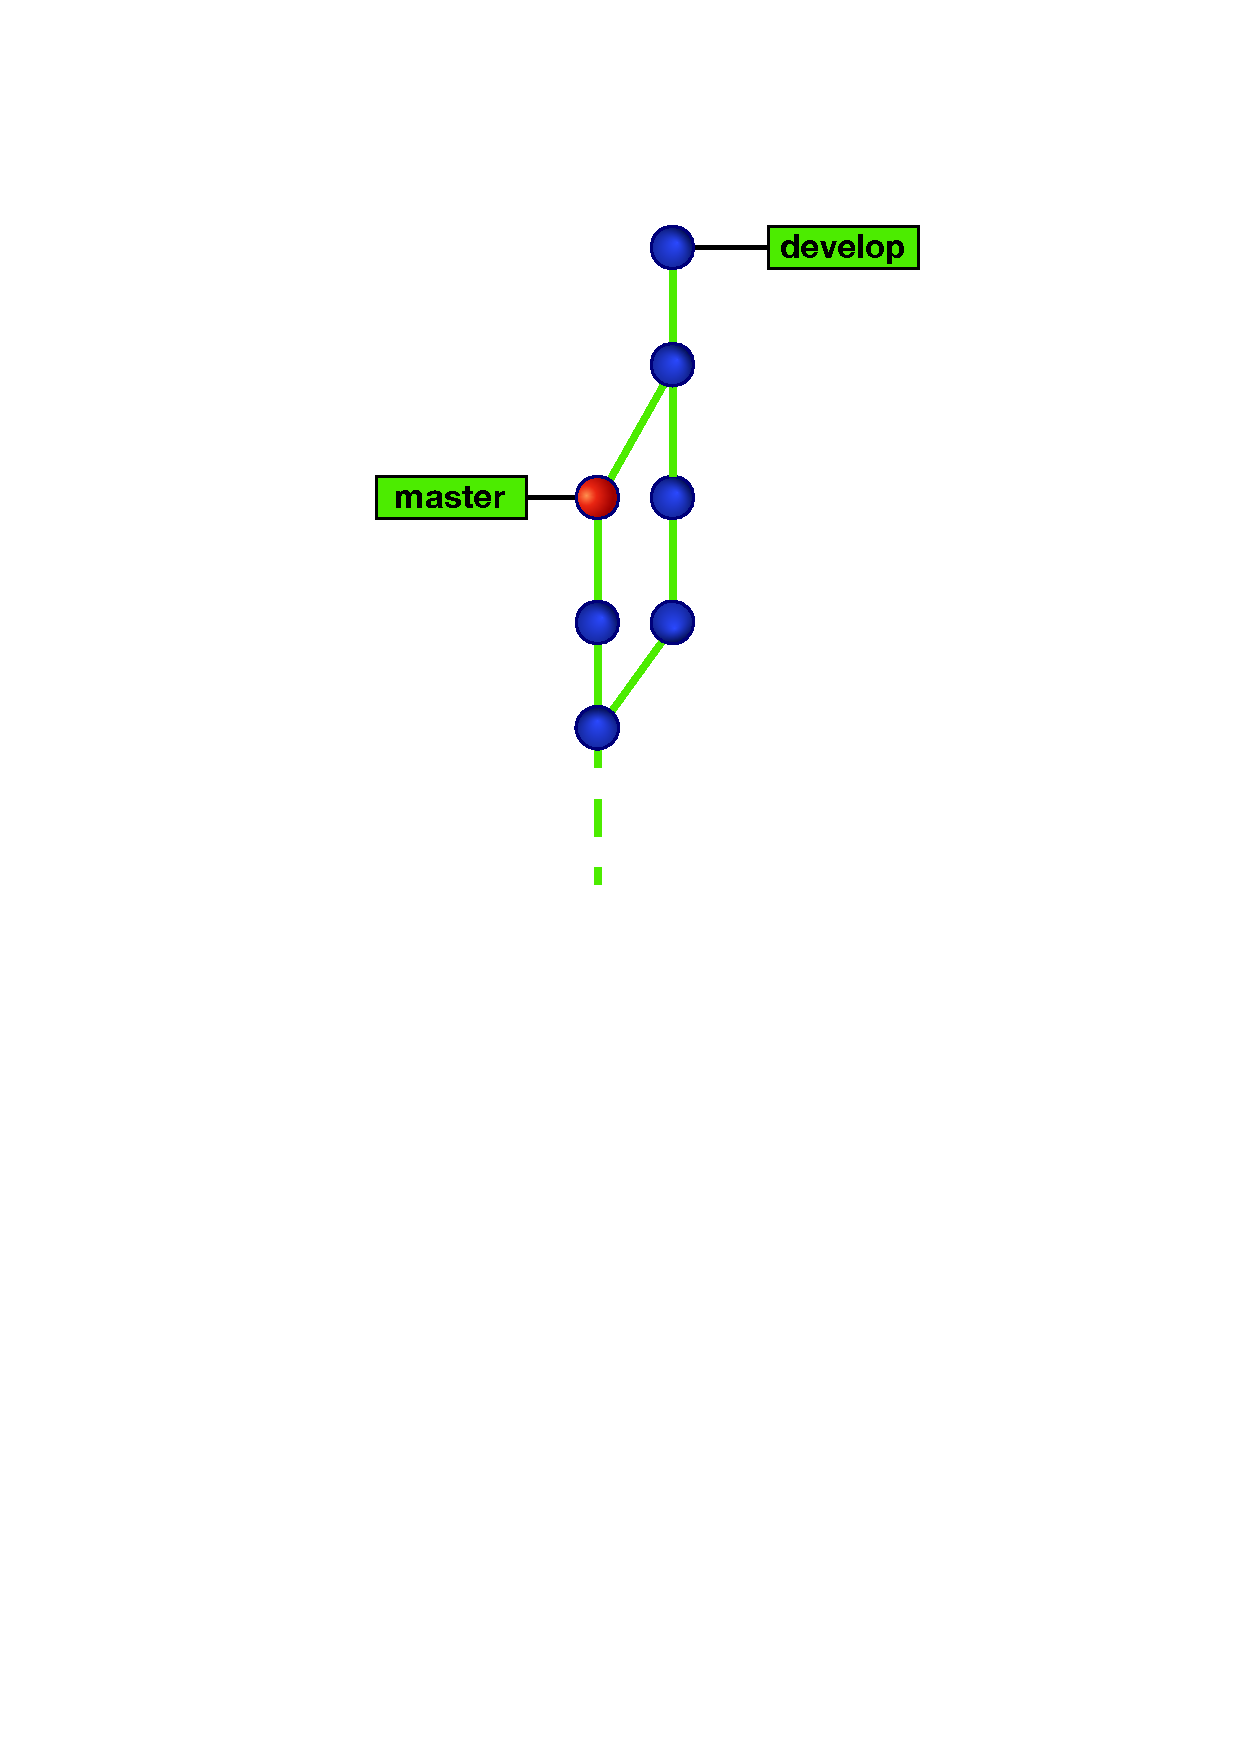
\includegraphics[width=1\textwidth]{images/branch11.pdf}
\end{column}

\begin{column}{0.60\textwidth}
\texttt{git\ checkout\ master}
\end{column}
\end{columns}

\end{frame}

\begin{frame}[fragile]{%
\protect\hypertarget{exemple-1212}{%
Exemple (12/12)}}

\begin{columns}[T]
\begin{column}{0.40\textwidth}
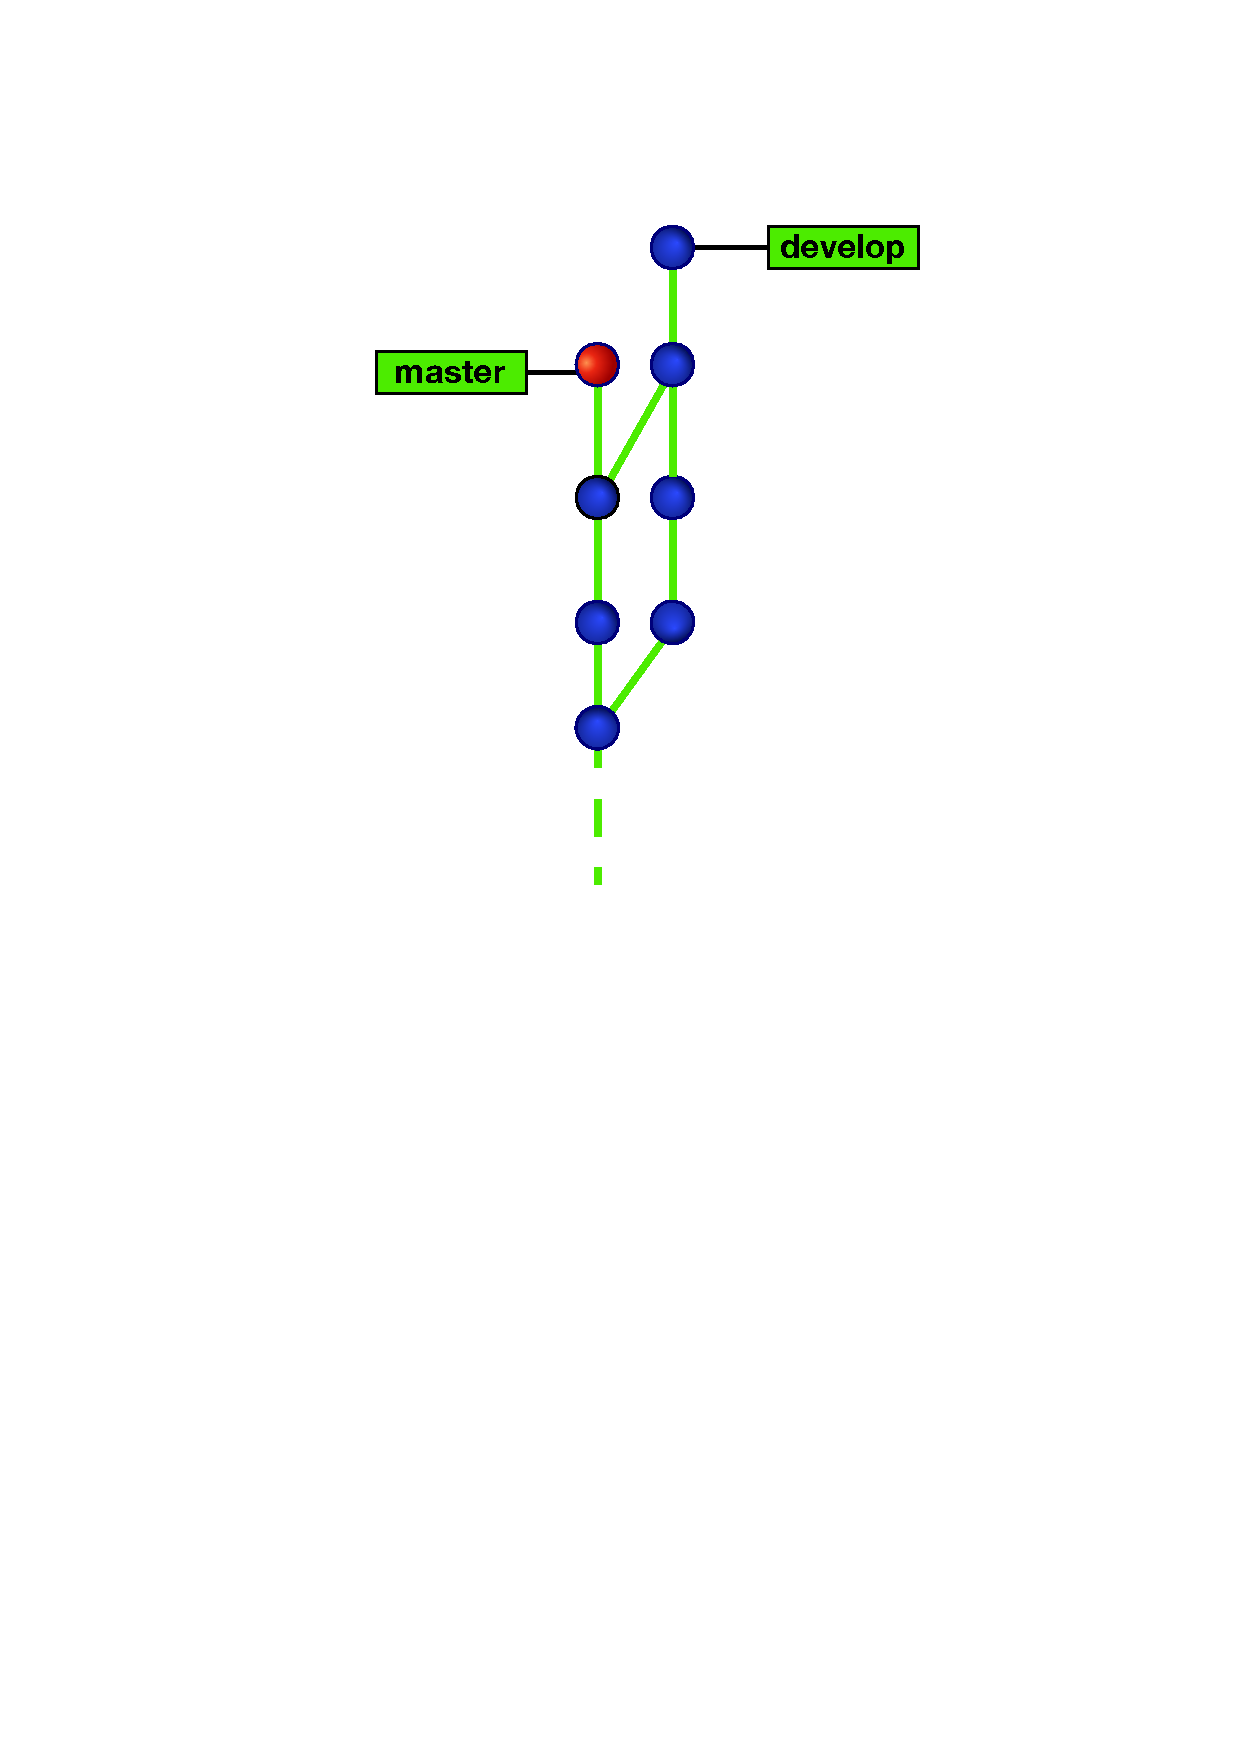
\includegraphics[width=1\textwidth]{images/branch12.pdf}
\end{column}

\begin{column}{0.60\textwidth}
\texttt{git\ commit}
\end{column}
\end{columns}

\end{frame}

\begin{frame}[fragile]{%
\protect\hypertarget{comment-git-fusionne-t-il-les-fichiers}{%
Comment git fusionne-t-il les fichiers ?}}

Si le même fichier est modifié dans les deux branches, git doit
fusionner deux variantes :

\begin{itemize}
\tightlist
\item
  les \textbf{fichiers texte} sont fusionnés ligne par ligne

  \begin{itemize}
  \tightlist
  \item
    les lignes modifiées dans une seule branche sont automatiquement
    fusionnées
  \item
    si une ligne est modifiée dans deux branches, \texttt{git} rapporte
    un conflit
  \item
    les zones de conflits sont repérées par
    \texttt{\textless{}\textless{}\textless{}\textless{}\textless{}\textless{}\textless{}}
    et
    \texttt{\textgreater{}\textgreater{}\textgreater{}\textgreater{}\textgreater{}\textgreater{}\textgreater{}}
  \end{itemize}
\item
  les \textbf{fichiers binaires} génèrent toujours un conflit
\item
  on résout alors les conflits manuellement (en éditant les fichiers)
\item
  \texttt{git} refusera le commit tant que tous les conflits ne sont pas
  réglés
\end{itemize}

\end{frame}

\begin{frame}[fragile]{%
\protect\hypertarget{exemple-de-fusion-manuelle}{%
Exemple de fusion manuelle}}

\begin{verbatim}
Lorsque l'enfant paraît, le cercle de famille
Applaudit à grands cris.
Son doux regard qui brille
Fait briller tous les yeux,
<<<<<<< HEAD
Et les plus tristes fronds, les plus souillés peut-être,
=======
Et les plus tristes fronts, les plus mouillés peut-être,
>>>>>>> conflit
Se dérident soudain à voir l'enfant paraître,
Innocent et joyeux.

Victor Hugo
\end{verbatim}

\end{frame}

\begin{frame}{%
\protect\hypertarget{plus-simple-avec-un-outil-appropriuxe9-atom}{%
Plus simple avec un outil approprié (Atom) !}}

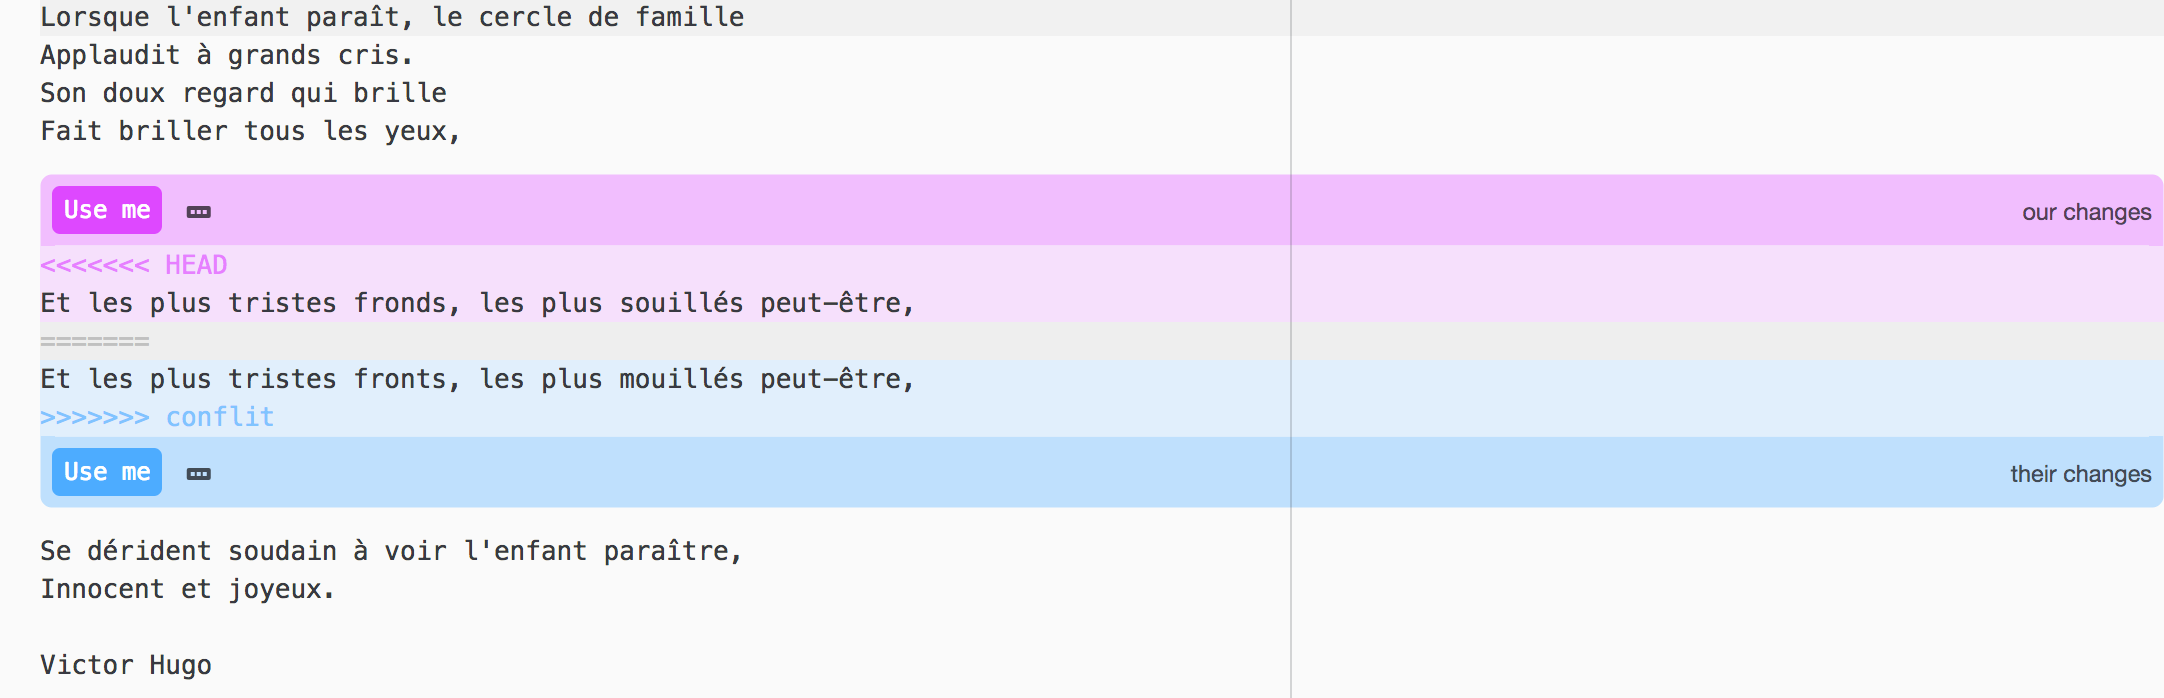
\includegraphics[width=1\textwidth]{images/fusion.png}

\end{frame}

\hypertarget{travailler-uxe0-plusieurs-sur-git}{%
\section{Travailler à plusieurs sur
git}\label{travailler-uxe0-plusieurs-sur-git}}

\begin{frame}[fragile]{%
\protect\hypertarget{introduction}{%
Introduction}}

\begin{itemize}
\tightlist
\item
  il n’existe pas une façon unique de travailler à plusieurs sur
  \texttt{git}
\item
  dans tous les cas, il faut un serveur \emph{central}
\item
  ce serveur peut être :

  \begin{itemize}
  \tightlist
  \item
    monté par vous-même ou votre organisation
  \item
    un provider quelconque (github est le plus connu)
  \end{itemize}
\item
  dans tous les cas, il faut apprendre quelques commandes
  \texttt{git}supplémentaires
\end{itemize}

\end{frame}

\begin{frame}[fragile]{%
\protect\hypertarget{le-workflow-centralisuxe9}{%
Le workflow centralisé}}

\begin{itemize}
\tightlist
\item
  Fonctionne à peu près comme \texttt{svn}
\item
  permet à tout le monde de travailler plus ou moins en même temps
\item
  la gestion des conflits est du ressort de chacun des développeurs
\item
  il faut avoir des droits sur le serveur pour attribuer à chaque
  développeur
\item
  pas très \emph{scalable}
\end{itemize}

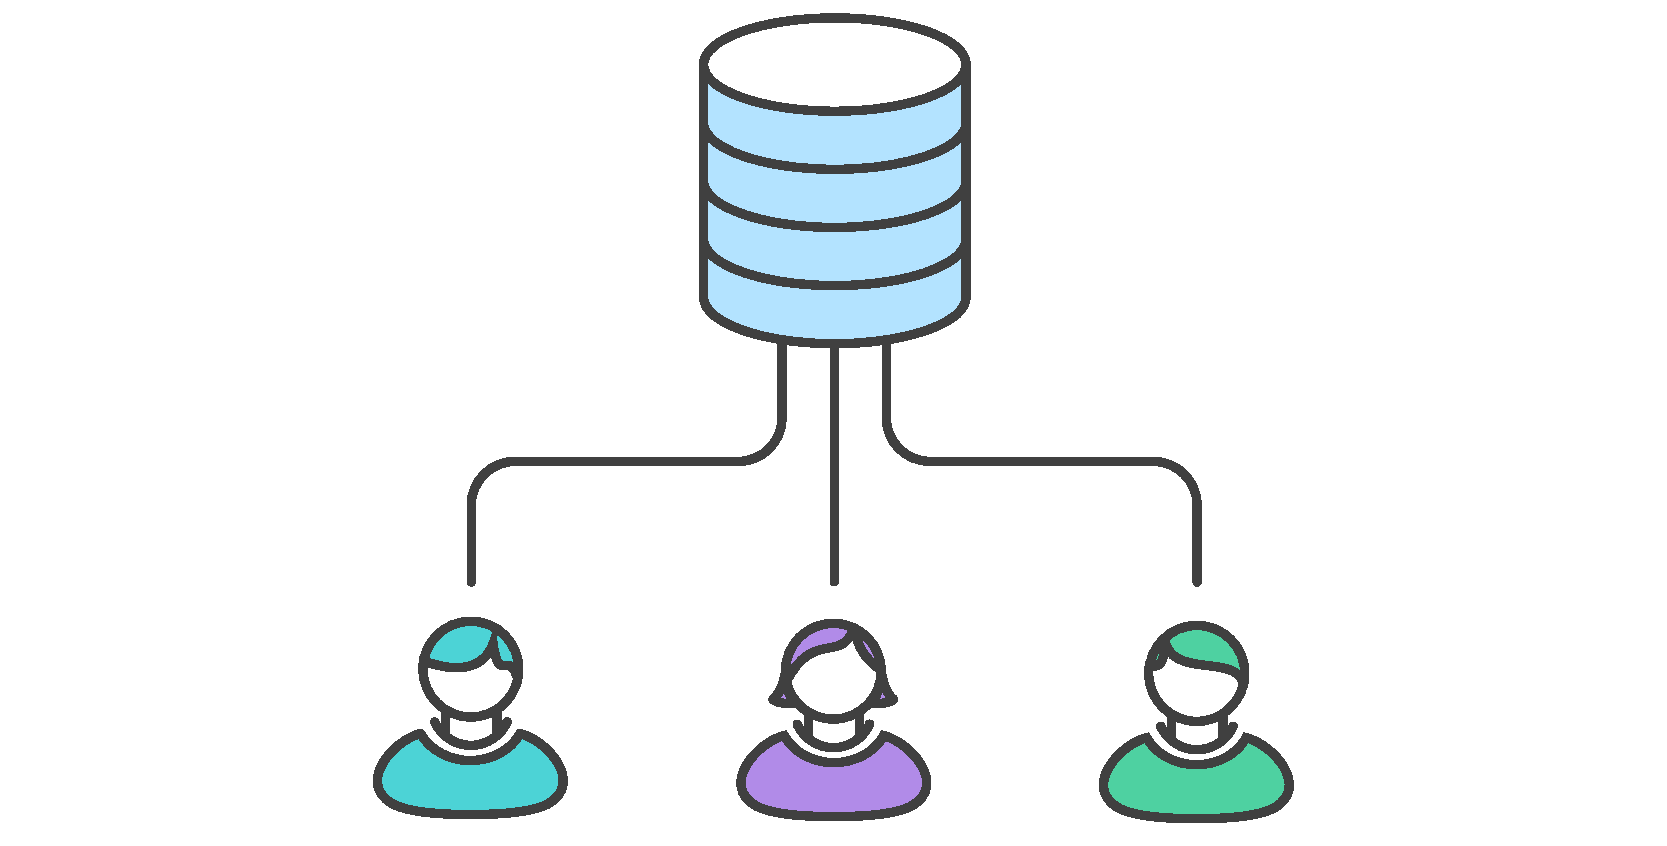
\includegraphics[width=0.5\textwidth]{images/centralise.pdf}

\end{frame}

\begin{frame}{%
\protect\hypertarget{illustration-15}{%
Illustration (1/5)}}

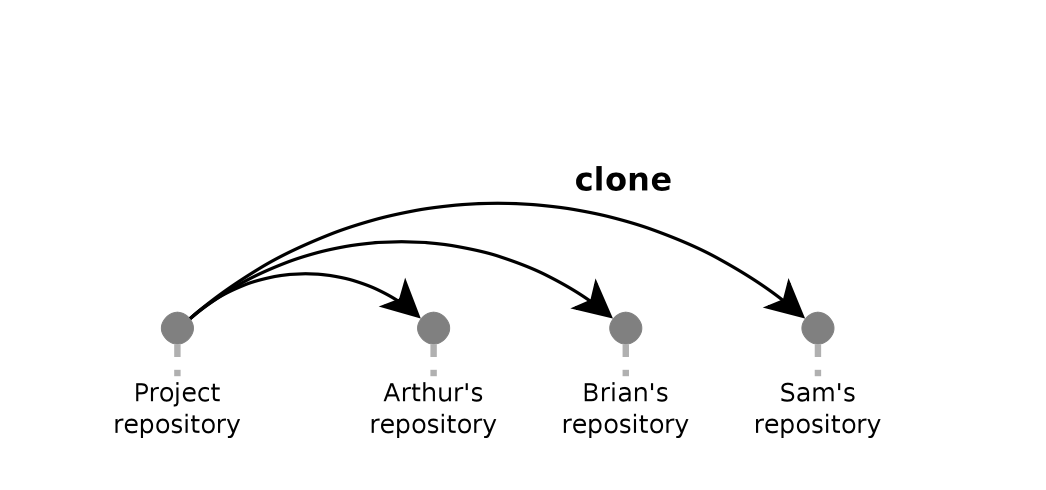
\includegraphics[width=0.8\textwidth]{images/centralise-1.png}

\end{frame}

\begin{frame}{%
\protect\hypertarget{illustration-25}{%
Illustration (2/5)}}

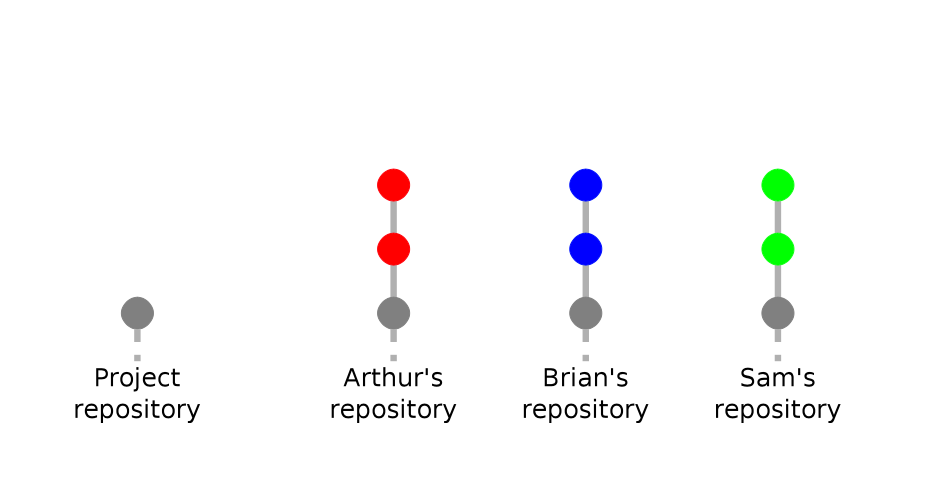
\includegraphics[width=0.8\textwidth]{images/centralise-2.png}

\end{frame}

\begin{frame}{%
\protect\hypertarget{illustration-35}{%
Illustration (3/5)}}

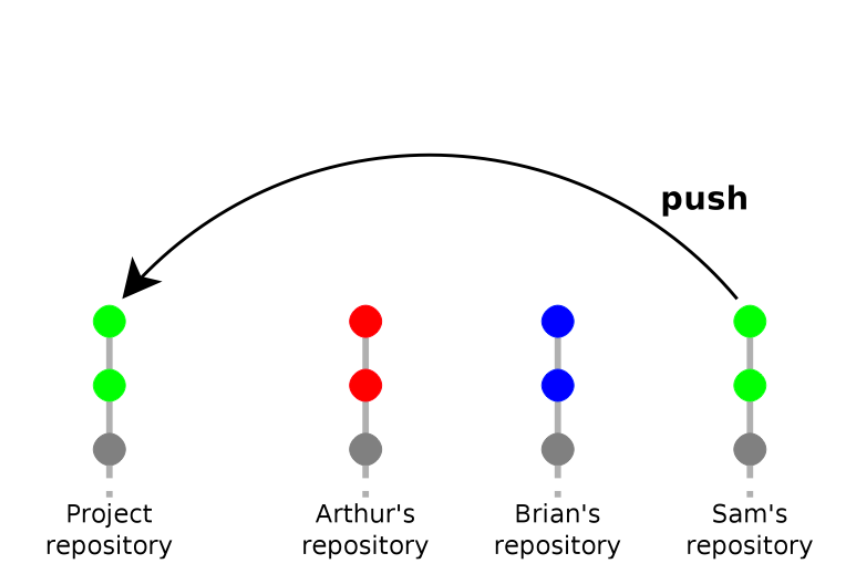
\includegraphics[width=0.8\textwidth]{images/centralise-3.png}

\end{frame}

\begin{frame}{%
\protect\hypertarget{illustration-45}{%
Illustration (4/5)}}

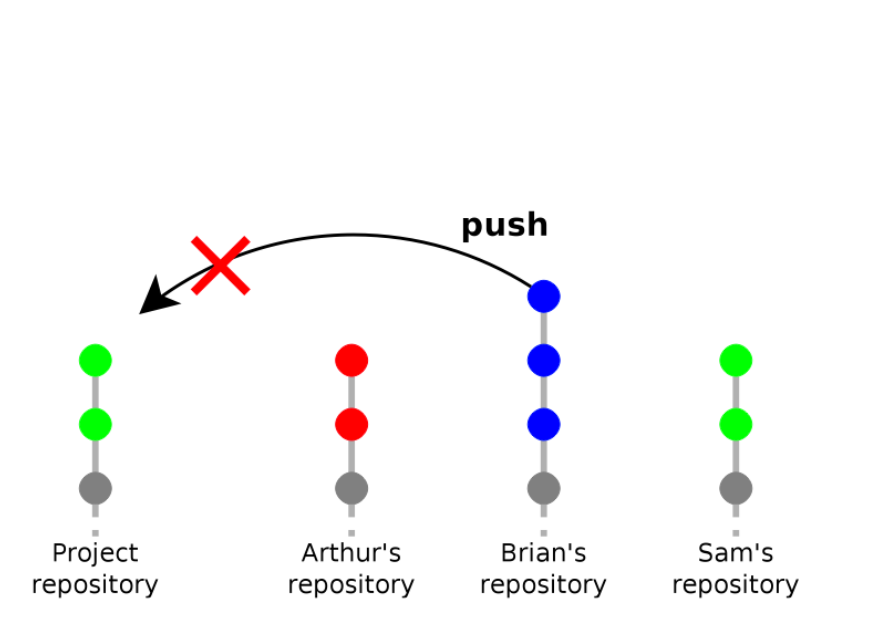
\includegraphics[width=0.8\textwidth]{images/centralise-4.png}

\end{frame}

\begin{frame}{%
\protect\hypertarget{illustration-55}{%
Illustration (5/5)}}

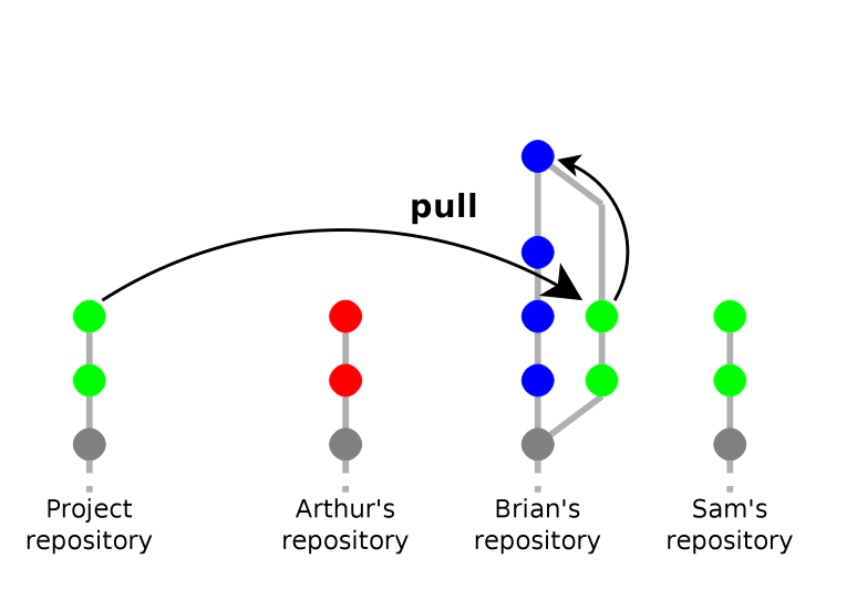
\includegraphics[width=0.8\textwidth]{images/centralise-5.png}

\end{frame}

\begin{frame}{%
\protect\hypertarget{exemple-classique-de-fauxe7on-de-travailler}{%
exemple classique de façon de travailler}}

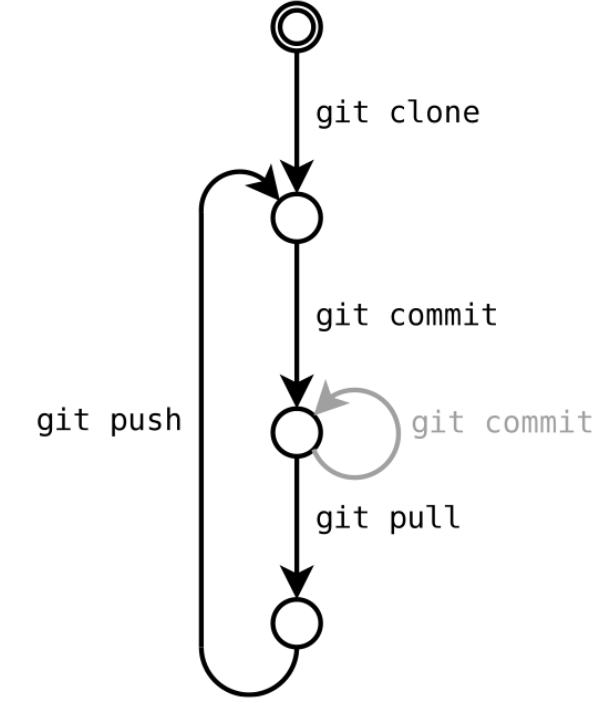
\includegraphics[width=0.5\textwidth]{images/centralise-typique.png}

\end{frame}

\begin{frame}[fragile]{%
\protect\hypertarget{commandes}{%
Commandes}}

\texttt{git\ clone\ ssh://user@host/path/to/repo.git}

\begin{itemize}
\tightlist
\item
  l’URL peut être différente (github vous les fournit à copier/coller)
\item
  crée automatiquement un raccourci vers l’adresse locale appelé
  \texttt{origin}
\item
  le processus est ensuite classique, il se déroule en local

  \begin{itemize}
  \tightlist
  \item
    \texttt{git\ status}
  \item
    \texttt{git\ add}
  \item
    \texttt{git\ commit}
  \end{itemize}
\item
  \texttt{git\ push\ origin\ master}
\item
  mais ne pas oublier que les autres travaillent

  \begin{itemize}
  \tightlist
  \item
    \texttt{git\ pull}
  \end{itemize}
\end{itemize}

\end{frame}

\begin{frame}[fragile]{%
\protect\hypertarget{le-workflow-github}{%
Le workflow github}}

\begin{itemize}
\tightlist
\item
  vrai pour plusieurs hébergeurs \texttt{git} : github, bitbucket,
  gitlab\ldots{}
\item
  A tester par soi-même
\end{itemize}

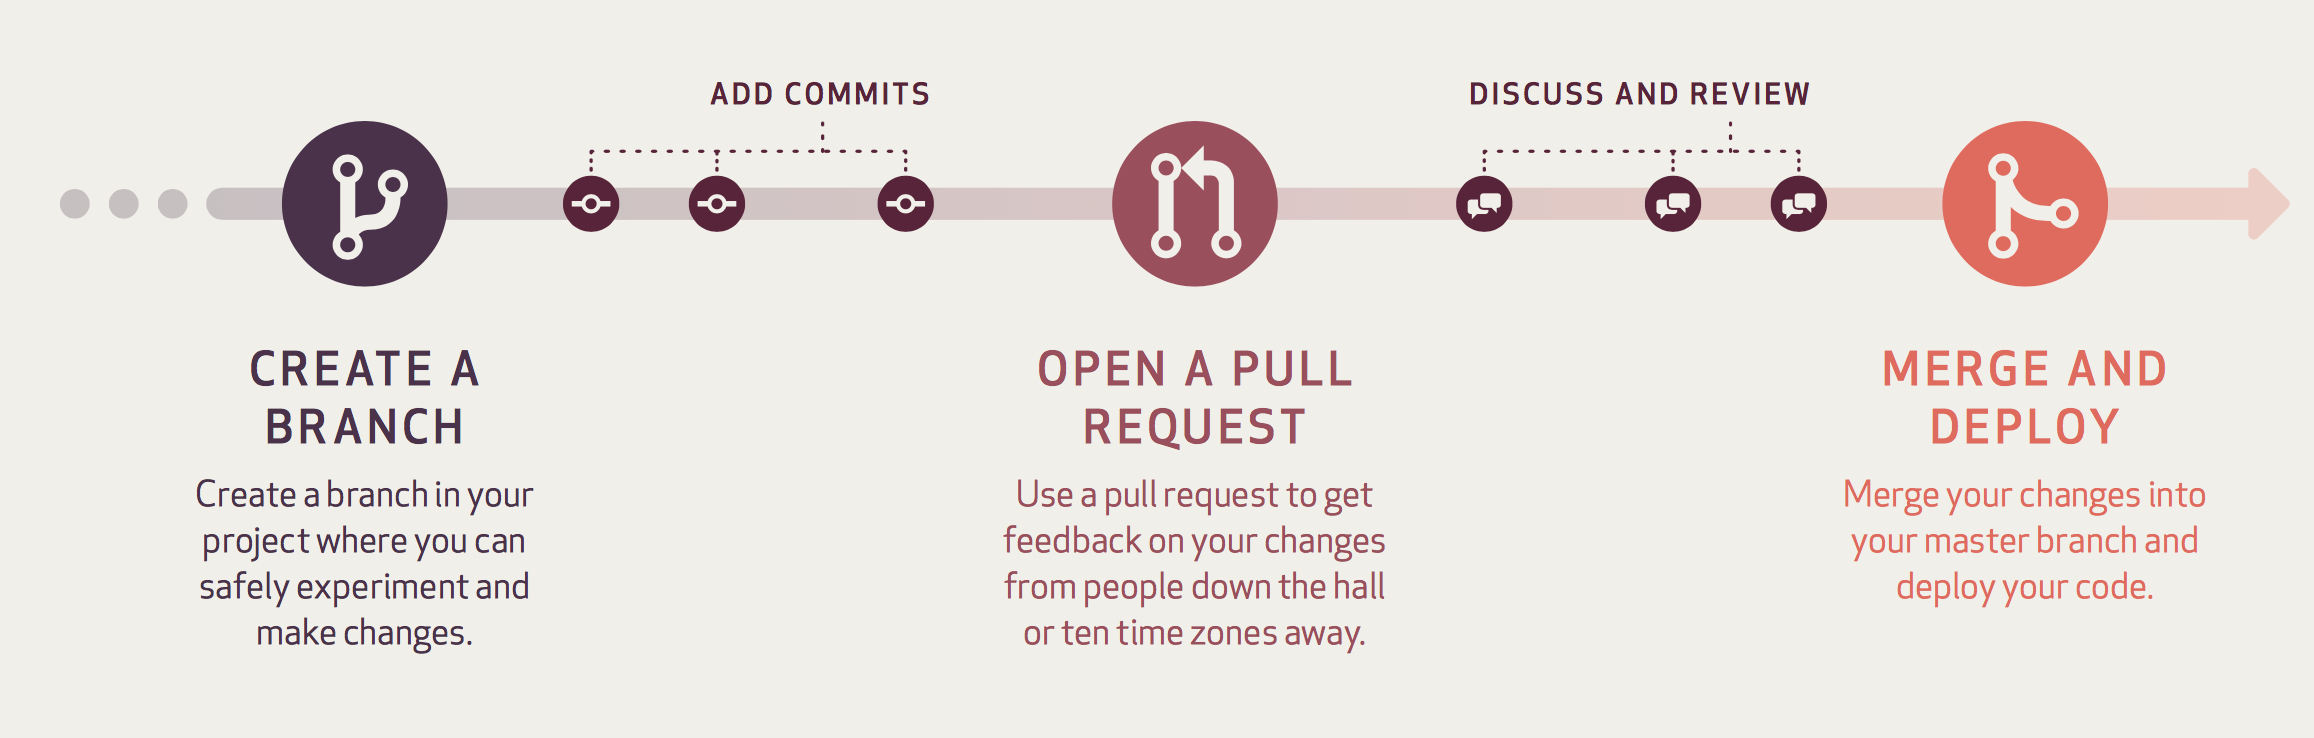
\includegraphics[width=1\textwidth]{images/github-workflow.png}

\end{frame}

\begin{frame}[fragile]{%
\protect\hypertarget{quelques-ruxe9fuxe9rences}{%
Quelques références}}

\begin{itemize}
\tightlist
\item
  The \texttt{git} book: http://git-scm.com/book
\item
  Documentation github : http://learn.github.com/
\item
  Documentation Atlassian/bitbucket :
  https://www.atlassian.com/git/tutorial
\end{itemize}

\end{frame}
